% !TEX program = xelatex
\documentclass[12pt, a4paper, oneside]{book}
%\documentclass[11pt, a4paper, oneside]{book}
%% Übersetzen als Entwurf
% \usepackage[entwurf]{bhtThesis}
%% Übersetzen für die Abgabe
\usepackage[abgabe]{bhtThesis}
\typeout{BHT-Abschlussarbeit V2.0 26.08.21 S.Tschirley}

\usepackage{blindtext}   %für Blindtext in Kapitel 2
\usepackage{listings}
\lstset{ 
  literate={ö}{{\"o}}1
           {ä}{{\"a}}1
           {ü}{{\"u}}1
           {Ö}{{\"O}}1
           {Ä}{{\"A}}1
           {Ü}{{\"U}}1
           {ß}{{\ss}}1
}
%%\usepackage{hyperref}
% \usepackage[demo]{graphicx}
% \usepackage[section]{placeins}
%%%%%%%%%%%%%%%%%%%%%%%%%%%%%%%%%%%%%%%%%%%%%%%%%%%%%%%%%%%%%%%%
% Mathstuff
\usepackage{caption}
\DeclareCaptionType{equ}[][]
\usepackage{amsmath}
%%%%%%%%%%%%%%%%%%%%%%%%%%%%%%%%%%%%%%%%%%%%%%%%%%%%%%%%%%%%%%%%
% Tablestuff
\usepackage{booktabs}
\usepackage{multirow}
% \newcommand{\ra}[1]{\renewcommand{\arraystretch}{#1}}
\usepackage{color, colortbl}
\definecolor{LightGray}{gray}{0.9}

%%%%%%%%%%%%%%%%%%%%%%%%%%%%%%%%%%%%%%%%%%%%%%%%%%%%%%%%%%%%%%%%
\usepackage{subcaption}
\usepackage{graphicx}

\usepackage{tikz}
\usepackage{pgfplots}
%Loading xcolor with dvipsnames
%\usepackage[dvipsnames]{xcolor}
%%%%%%%%%%%%%%%%%%%%%%%%%%%%%%%%%%%%%%%%%%%%%%%%%%%%%%%%%%%%%%%%
% Bibtex show urls
%\usepackage{url}
\usepackage{hyperref} 
% \usepackage[backend=biber,sorting=ynt]{biblatex}
%%%%%%%%%%%%%%%%%%%%%%%%%%%%%%%%%%%%%%%%%%%%%%%%%%%%%%%%%%%%%%%%
\usepackage{trsym}
%\usepackage{showkeys}
\usepackage{bytefield}

\graphicspath{
  {pictures/}
}

\version{0.1$\alpha$}    % word im Entwurf auf der Titelseite vermerkt
\datum{\today}
%%
%% Titel, Autor und Betreuer
%%
\fachbereich{VI -- Informatik und Medien -- Technische Informatik} 
\studiengang{Technische Informatik - Embedded Systems}
\autor{Gina Hortenbach}
\edvnr{897854}
\titel{Visuelle Odometrie zur Lokalisierung autonomer Fahrzeuge}
% \untertitel{Teil des CARS Forschungsprojekts}
\betreuerFeld{
  \begin{tabular}{lr}
    \multicolumn{2}{l}{\textbf{Gutachter}}\\
    Prof.~Dr.-Ing. V. Sommer & Berliner Hochschule für Technik\\
    Prof.~Dr.-Ing. H. Höfig & Berliner Hochschule für Technik
  \end{tabular}
}

% Remove "chapter x"
\usepackage{titlesec}
\titleformat{\chapter}{\normalfont\huge\bf}{\thechapter.}{20pt}{\huge\bf}
%%\renewcommand{\baselinestretch}{1.05} 

\usepackage{enumitem}


\begin{document}
\pagestyle{fancy}

%%
%% Berliner Hochschule für Technik --  Abschlussarbeit
%%
%% Titelseiten und Erklärungen 
%%
%%%%%%%%%%%%%%%%%%%%%%%%%%%%%%%%%%%%%%%%%%%%%%%%%%%%%%%%%%%%%%%%%%%%%

\maketitle
\clearpage
%\thispagestyle{empty}
% Rueckseite (leer)
%% 
~
% \newpage
% \vspace{10ex}
% \section*{Erklärung}
% Ich  versichere, dass  ich diese  Abschlussarbeit ohne  fremde  Hilfe selbstständig
% verfasst und  nur die  angegebenen Quellen und  Hilfsmittel benutzt  habe. Wörtlich
% oder dem  Sinn nach  aus anderen  Werken entnommene Stellen  sind unter  Angabe der
% Quellen kenntlich gemacht.
% \vspace{20ex}\\

% \hrule
% {\small{Datum}}\hfill{\small{Unterschrift}}


\noindent Hiermit erkläre ich,
	\begin{itemize}
	\item dass ich die vorliegende Arbeit selbstständig verfasst habe,
	\item dass keine anderen als die angegebenen Quellen benutzt und alle wörtlich oder sinngemä{\ss} aus anderen Werken übernommenen Aussagen als solche gekennzeichnet sind,
	\item dass die eingereichte Arbeit weder vollständig noch in wesentlichen Teilen Gegenstand eines anderen Prüfungsverfahrens gewesen ist,
	\item dass ich die Arbeit weder vollständig noch in Teilen bereits veröffentlicht habe und 
	\item dass ich mit der Arbeit keine Rechte Dritter verletze und die Universität von etwaigen Ansprüchen Dritter freistelle.
	\end{itemize}
% \vfill
\vspace*{8em}

\noindent\rule{6cm}{0.66pt}\\
%Berlin,{ den} \@date
Berlin,{ den \today}

\pagenumbering{roman}
\clearpage\newpage

%%
%% Abstract
%%
%%%%%%%%%%%%%%%%%%%%%%%%%%%%%%%%%%%%%%%%%%%%%%%%%%%%%%%%%%%%%%%%%%%%%

% Die Kurzfassung gibt  ein kurzes und prägnantes Bild der  gesamten Arbeit. Sie soll
% den  Leser  neugierig  machen  und  klarmachen,  was  zu  erwarten  ist.  Erreichte
% Ergebnisse werden kurz umrissen.

\section*{Kurzfassung}
In der vorliegenden Abschlussarbeit "Visuelle Odometrie zur Lokalisierung autonomer Fahrzeuge" wurde die gefahrene Trajektorie eines Fahrzeuges auf mehreren Teststrecken ausschlie{\ss}lich anhand von Kameradaten geschätzt. Die Testfahrten wurden zu unterschiedliche Licht- und Witterungsverhältnisse durchgeführt mit Streckenlängen bis zu 2 km. 
\newline

Ein Stereokamerasystem und ein RGB-D Kamerasystem wurden am Fahrzeug montiert und miteinander verglichen. Die Fahrzeugpose wurde für beide Kamerasysteme mit der selben merkmalsbasierten Visuellen Odometrie geschätzt. Projektive Geometrie und die Extraktion von Bildmerkmalen zählt daher zu den zentralen Themen der Arbeit. 
\newline

Als Testumgebung wurde der CARLA Simulator verwendet. Geschätzten Odometrie Daten werden in einem ROS2 Netzwerk veröffentlicht wodurch die Implementation hoch modular ist und problemlos in bestehende ROS2 basierte Systeme integriert werden kann. 
\newline

Insgesamt konnten Orientierung und Position mittels visueller Odometrie zuverlässig geschätzt werden, wobei das System mit den Daten der RGB-D Kamerasystem geringer Schätzfehler erzielte.  


%% eof

%%
%% Abstract
%%
%%%%%%%%%%%%%%%%%%%%%%%%%%%%%%%%%%%%%%%%%%%%%%%%%%%%%%%%%%%%%%%%%%%%%


\section*{Abstract}
In the present thesis "Visual odometry for the localization of autonomous vehicles", the driven trajectory of a vehicle on test routes was estimated exclusively using camera data. The test drives were carried out under different light and weather conditions with distances of up to 2 km.
\newline

A stereo camera system and an RGB-D camera system were mounted on the vehicle and recorded together. Vehicle pose was estimated for both camera systems using the same feature-based visual odometry. Projective geometry and the extraction of image features are therefore among the most important topics of the work.
\newline 

The CARLA simulator was used as a test environment. Estimated odometry data is published on a ROS2 network, making the implementation highly modular and easily integrated into ROS2 based systems.
\newline 

Overall, orientation and position could be reliably estimated using visual odometry, with the system using the data from the RGB-D camera system achieving lower estimation errors.


%% eof


\tableofcontents

\listoffigures
\newpage

% %%
%% Abstract
%%
%%%%%%%%%%%%%%%%%%%%%%%%%%%%%%%%%%%%%%%%%%%%%%%%%%%%%%%%%%%%%%%%%%%%%

% Die Kurzfassung gibt  ein kurzes und prägnantes Bild der  gesamten Arbeit. Sie soll
% den  Leser  neugierig  machen  und  klarmachen,  was  zu  erwarten  ist.  Erreichte
% Ergebnisse werden kurz umrissen.

\section*{Kurzfassung}
In der vorliegenden Abschlussarbeit "Visuelle Odometrie zur Lokalisierung autonomer Fahrzeuge" wurde die gefahrene Trajektorie eines Fahrzeuges auf mehreren Teststrecken ausschlie{\ss}lich anhand von Kameradaten geschätzt. Die Testfahrten wurden zu unterschiedliche Licht- und Witterungsverhältnisse durchgeführt mit Streckenlängen bis zu 2 km. 
\newline

Ein Stereokamerasystem und ein RGB-D Kamerasystem wurden am Fahrzeug montiert und miteinander verglichen. Die Fahrzeugpose wurde für beide Kamerasysteme mit der selben merkmalsbasierten Visuellen Odometrie geschätzt. Projektive Geometrie und die Extraktion von Bildmerkmalen zählt daher zu den zentralen Themen der Arbeit. 
\newline

Als Testumgebung wurde der CARLA Simulator verwendet. Geschätzten Odometrie Daten werden in einem ROS2 Netzwerk veröffentlicht wodurch die Implementation hoch modular ist und problemlos in bestehende ROS2 basierte Systeme integriert werden kann. 
\newline

Insgesamt konnten Orientierung und Position mittels visueller Odometrie zuverlässig geschätzt werden, wobei das System mit den Daten der RGB-D Kamerasystem geringer Schätzfehler erzielte.  


%% eof

% %%
%% Abstract
%%
%%%%%%%%%%%%%%%%%%%%%%%%%%%%%%%%%%%%%%%%%%%%%%%%%%%%%%%%%%%%%%%%%%%%%


\section*{Abstract}
In the present thesis "Visual odometry for the localization of autonomous vehicles", the driven trajectory of a vehicle on test routes was estimated exclusively using camera data. The test drives were carried out under different light and weather conditions with distances of up to 2 km.
\newline

A stereo camera system and an RGB-D camera system were mounted on the vehicle and recorded together. Vehicle pose was estimated for both camera systems using the same feature-based visual odometry. Projective geometry and the extraction of image features are therefore among the most important topics of the work.
\newline 

The CARLA simulator was used as a test environment. Estimated odometry data is published on a ROS2 network, making the implementation highly modular and easily integrated into ROS2 based systems.
\newline 

Overall, orientation and position could be reliably estimated using visual odometry, with the system using the data from the RGB-D camera system achieving lower estimation errors.


%% eof

% \clearpage
\newpage\clearpage

%%\setlist[description]{font=\normalfont\itshape\bold\space}

\pagenumbering{arabic}
%%%%%%%%%%%%%%%%%%%%%%%%%%%%%%%%%%%%%%%%%%%%%%%%%%%%%%%%%%%%%%%
%% Die Kapitel der Arbeit
%%
%% Abstract
%%
%%%%%%%%%%%%%%%%%%%%%%%%%%%%%%%%%%%%%%%%%%%%%%%%%%%%%%%%%%%%%%%%%%%%%

% Die Kurzfassung gibt  ein kurzes und prägnantes Bild der  gesamten Arbeit. Sie soll
% den  Leser  neugierig  machen  und  klarmachen,  was  zu  erwarten  ist.  Erreichte
% Ergebnisse werden kurz umrissen.

\section*{Kurzfassung}
In der vorliegenden Abschlussarbeit "Visuelle Odometrie zur Lokalisierung autonomer Fahrzeuge" wurde die gefahrene Trajektorie eines Fahrzeuges auf mehreren Teststrecken ausschlie{\ss}lich anhand von Kameradaten geschätzt. Die Testfahrten wurden zu unterschiedliche Licht- und Witterungsverhältnisse durchgeführt mit Streckenlängen bis zu 2 km. 
\newline

Ein Stereokamerasystem und ein RGB-D Kamerasystem wurden am Fahrzeug montiert und miteinander verglichen. Die Fahrzeugpose wurde für beide Kamerasysteme mit der selben merkmalsbasierten Visuellen Odometrie geschätzt. Projektive Geometrie und die Extraktion von Bildmerkmalen zählt daher zu den zentralen Themen der Arbeit. 
\newline

Als Testumgebung wurde der CARLA Simulator verwendet. Geschätzten Odometrie Daten werden in einem ROS2 Netzwerk veröffentlicht wodurch die Implementation hoch modular ist und problemlos in bestehende ROS2 basierte Systeme integriert werden kann. 
\newline

Insgesamt konnten Orientierung und Position mittels visueller Odometrie zuverlässig geschätzt werden, wobei das System mit den Daten der RGB-D Kamerasystem geringer Schätzfehler erzielte.  


%% eof

%%
%% Abstract
%%
%%%%%%%%%%%%%%%%%%%%%%%%%%%%%%%%%%%%%%%%%%%%%%%%%%%%%%%%%%%%%%%%%%%%%


\section*{Abstract}
In the present thesis "Visual odometry for the localization of autonomous vehicles", the driven trajectory of a vehicle on test routes was estimated exclusively using camera data. The test drives were carried out under different light and weather conditions with distances of up to 2 km.
\newline

A stereo camera system and an RGB-D camera system were mounted on the vehicle and recorded together. Vehicle pose was estimated for both camera systems using the same feature-based visual odometry. Projective geometry and the extraction of image features are therefore among the most important topics of the work.
\newline 

The CARLA simulator was used as a test environment. Estimated odometry data is published on a ROS2 network, making the implementation highly modular and easily integrated into ROS2 based systems.
\newline 

Overall, orientation and position could be reliably estimated using visual odometry, with the system using the data from the RGB-D camera system achieving lower estimation errors.


%% eof


\chapter{Einleitung}
\section{Motivation - Forschungsprojekt CARS}
Die vorliegende Abschlussarbeit ist im Rahmen des "Cooperative Autonomy based on Reliable Services"  (CARS) Forschungsprojekts entstanden. CARS ist ein von der IFAF Gefördertes Projekt unter der Leitung von Prof. Dr.-Ing. Carsten Thomas (HTW Berlin) und Prof. Dr.-Ing. Volker Sommer (BHT). Der Forschungsschwerpunkt liegt auf der Erhöhung der Sicherheit hochautonomen Fahrens. Als Ansatz werden hierfür Verfahren für die Fahrzeug-zu-Fahrzeug Kommunikation erforscht.
\newline 

Die Fahrzeuge sollen gegenseitig interne und externe Zuständen austauschen. Dadurch soll ein umfangreiches und zuverlässiges Situationsbewusstsein der einzelnen Systeme erreicht werden. 
\newline 

Die Lokalisierung durch Visuelle Odometrie kann die Position und Orientierung eines Fahrzeugs schätzen. Aus dieser Information ergibt sich auch die Trajektorie. Neben dem Austausch mit anderen Systemen, könne die Daten intern genutzt werden. Beispielsweise kann Visuelle Odometrie das  Front-End für Simultaneous Localization And Mapping (SLAM) stellen.

\section{Ziel der Arbeit}
Im Rahmen der Abschlussarbeit soll ein System implementiert werden, dass mittels Visueller Odometrie die Position und Orientierung (Pose) eines Fahrzeugs schätzt. Die Implementierung soll sich mit dem CARLA Simulator nutzen lassen und Odometriedaten innerhalb eines ROS2 Netzwerks zur Verfügung stellen können.

Die Schätzung der Pose soll ausschlie{\ss}lich auf Kameradaten basieren, es wird nicht auf andere Umgebungsdaten des Simulators zugegriffen. 

Für eine Software Implementierung sollen zwei Kamera-Setups verglichen werden; ein Stereokamera Aufbau mit zwei RGB Kamerasensoren und ein RGB-D Setup bestehend aus einer RGB und ToF Kamera.
%%
% \section{Stand der Technik und Verwandte Arbeiten}
 
% !TEX program = xelatex
\chapter{Grundlagen}
\label{ch:basics}

\section{Lokalisierungsverfahren}

Lokalisieren bedeutet immer, eine Pose innerhalb einer Umgebung zu bestimmen. Bei einigen Verfahren ist die Umgebung bekannt weil eine Karte gegeben ist, bei anderen ist die Umgebung unbekannt.
\newline

Prinzipiell werden Lokalisierungsverfahren anhand der Aufgabenstellung in zwei Kategorien unterschieden. Zum einen gibt es globale Verfahren und zum anderen Position Tracking bzw lokale Verfahren. Die Assoziation global und lokal bezieht sich auf das Koordinatensystem bzw Frame zu dem Bezug genommen wird.

\subsection{Globale Lokalisierung}

Globale Lokalisierung schätzt die Pose im globalen Referenzsystem, d.h. in Bezug zum Koordinatenursprung der Umgebungskarte. Dabei müssen die Wahrscheinlichkeiten für mögliche Posen geschätzt werden. Ein bekanntes Beispiel für globale Lokalisierungsverfahren ist die Markov Lokalisation.
\newline

Eine Aufgabe, in dem die globalen Lokalisierung angewendet wird, ist die Ermittelung der Startposition. Denn autonome Agenten müssen sich häufig orientieren, nachdem sie durch externe Kräfte bewegt wurden. Globale Lokalisierung löst beispielsweise das Kidnapped-Robot Problem, bei dem der Agent plötzlich versetzt wurde oder bestimmt den Zustand nach dem Anschalten. Der Wake-Up eines Roboters zählt als ein Sonderfall des Kidnapped-Roboters, wobei dem Agenten hier i.d.R. bekannt ist, dass sich seine Position verändert hat.
\newline

Globalen Lokalisierungsverfahren müssen also in der Lage sein auch gro{\ss}e Positionsänderungen kompensiert zu können. \cite{locFox}


\subsection{Position Tracking}
Beim Position Tracking ist die Ausgangsposition in der Regel ungefähr bekannt und es sollen vor allem odometrische Fehler korrigiert werden. Der Referenzrahmen des position Tracking ist lokal und muss in einem weiteren Schritt in das globalen (Welt) Koordinatensystem transformiert werden. 
\newline

Für das Position Tracking wird die Pose inkrementell, von Frame zu Frame, ermittelt. Daher führen zu gr{\ss}e Änderungen zwischen zwei Zuständen zum Ausfall und die Schätzung muss abgebrochen werden.
\newline

Visuelle Odometrie zählt zu den Position Tracking Verfahren. Die Startposition wird als Koordinatenursprung des lokalen Bezugssystems gesetzt. Die Odometrieschätzung der aktuellen Pose bezieht sich immer auf die vorherige Pose. 

%%%%%%%%%%%%%%%%%%%%%%%%%%%%%%%%%%%%%%%%%%%%%%%%%%%
\section{3-D Strukturen und Kamerapose aus 2-D Bildern}
In den vergangenen 30 Jahren wurde viel Forschung im Bereich der Computer Vision als ein Teilgebiet der autonomen Robotik betrieben. Werden die Umgebungsinformationen teilweise oder ausschlie{\ss}lich aus Kamerasensoren erhalten, können geometrische Modelle aufgestellt werden um Informationen aus den Bildern zu gewinnen. Grundsätzlich soll die Kamera Pose aus Pixelinformationen hergeleitet werden. Eine Grundlage hierfür bildet die Korrespondenzanalyse, für die Merkmale aus den Bildern extrahiert werden müssen. Durch Bildkorrespondenzen kann eine Beziehung zwischen Bildern und zwischen Kamera und Umwelt hergestellt werden. Beim Umgang mit Bildkorrespondenzen werden Methoden der Projektiven- und Epipolargeometrie herangezogen.
\begin{figure}[!ht]
  \centering
  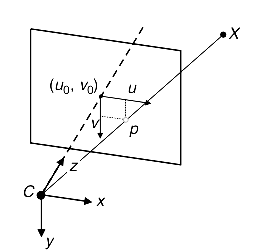
\includegraphics[width=0.4\textwidth]{pictures/02_2dpane.png}
  \caption[Abbildung von 3-D zu 2-D]{Abbildung einer 3-D Punktes X auf den 2-D Punkt p der Bildebene. (Scaramuzza, 2011 \cite{ScFrVO})}
  \label{fig:2dpane}
\end{figure}

Transformationen aus der projektiven Geometrie können im Alltag regelmä{\ss}ig auf Fotos beobachtet werden.  Beispielsweise erscheint ein Kreis je nach Perspektive, aus der er Abgebildet wurde, in einem Bild als Ellipse. Der Kreis wurde transformiert.
\newline

Durch Kamerasensoren werden Objekte aus dem 3-Dimensionalen Raum, der 'Welt', auf die 2-Dimensionalen Bildebene des Kamerabildes abgebildet. Dabei bleiben fast keine Eigenschaften der transformierten Objekte erhalten. Wie beim bereits aufgeführten Beispiel Kreis als Ellipse werden Objekte deformiert. Die einzige Eigenschaft, die erhalten bleibt, ist die Geradentreue. D.h. gerade Linien bleiben auch im Projektiven Raum immer gerade Linien.
% 
%%%%%%%%%%%%%%%%%%%%%%%%%%%%%%%%%%%%%%%%%%%%%%%%%%%
\subsection{Koordinatensysteme}
Bekannt ist der Euklidische Raum und die Euklidische Geometrie als Beschreibung von Winkeln und Formen von Objekten. Meistens werden Punkte des euklidischen Raumes im kartesischen Koordinatensystem dargestellt. Ein Problem im Modell der euklidischer Geometrie sind parallele Linien. Als Sonderfall wird angenommen, das sich parallele Linien im Unendlichen schneiden. Obwohl es tatsächlich im Euklidischen Raum keine Punkte im Unendlichen gibt.
\newline 

Der Projektive Raum ist die Transformation des Euklidischen Raums durch Einführung der Punkte im Unendlichen. Die Punkte werden dort als ideale Punkte oder Fernpunkte bezeichnet. Auch Räume sind in der geometrischen Betrachtung Objekte, die rotiert, verschoben oder gestreckt werden können.
\newline
\begin{figure}[!ht]
  \begin{subfigure}[t]{0.45\textwidth}
    \centering
    \begin{equation}
      T_{rotation}(\theta) = 
      \begin{pmatrix}
        cos \theta & -sin \theta \\
        sin \theta & cos \theta 
      \end{pmatrix}
    \end{equation}
    \caption*{Transformation Rotation für 2-D}
    \end{subfigure}
  \hfill
  \begin{subfigure}[t]{0.45\textwidth}
    \centering
    \begin{equation}
      T_{scale}(S) = 
      \begin{pmatrix}
        Sx & 0 \\
        0 & Sy 
      \end{pmatrix}
    \end{equation}
    \caption*{Transformation Verschiebung für 2-D}
  \end{subfigure}
  \label{fig:lintrans}
\end{figure}

Transformationen sind Operationen die auf alle Objekte angewendet werden können, also auf den Raum ebenso wie auf den Punkt. Verschiebung und Rotation zählen zu den Lineartransformationen und lassen sich daher durch Matrizen beschreiben.

\subsubsection{Homogene Koordinaten}
Die Translation, eine wichtige Transformation die für Lokalisierung benötigt wird, ist nicht linear. Um Translation in Matritzenschreibweise darstellen zu können, muss von kartesischen Koordinaten $(x ,y)$ zu homogenen Koordinaten $(x, y, 1)$ übergegangen werden. Dabei wird ein Vektor um eine weitere Komponente $w = 1$ erweitert. Es handelt sich bei homogenen Koordinaten um eine andere Schreibweise, nicht um eine Veränderung der Dimension. Alle Punkte $(kx, ky, k)$ sind gleich, für $k \neq 0$. 

Eine Rücktransformation von homogenen Koordinaten zu kartesischen erfolgt durch division von $(x,y)$ durch $k$. 

% %
\begin{figure}[!ht]
  \centering
  \begin{subfigure}[t]{0.4\textwidth}
    \centering
    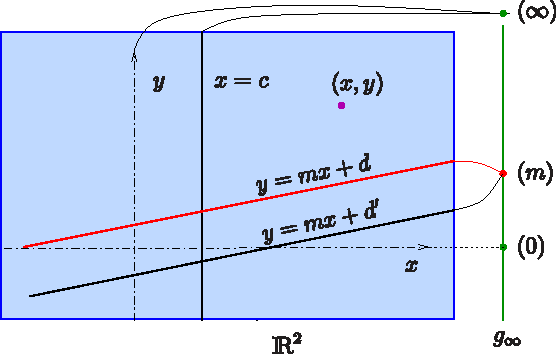
\includegraphics[width=\textwidth]{pictures/02_Projebeneinhomkoords.pdf}
    \caption[Projektive Ebene]{Die Projektive Ebene}
    \label{fig:y equals x}
  \end{subfigure}
  \hfill
  \begin{subfigure}[t]{0.55\textwidth}
    \centering
    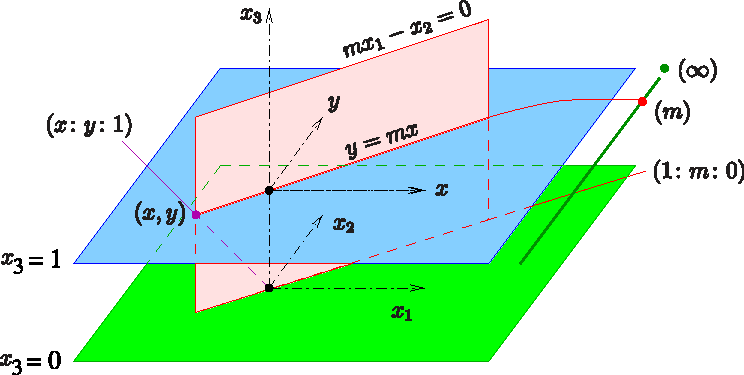
\includegraphics[width=\textwidth]{pictures/02_Projebenehomkoords.pdf}
    \caption[Urspungsgerade der inhomogenen Koordinaten]{Allen inhomogenen Geraden kann eine gemeinsame Ursprungsgerade $(1:m:0)$ zugeordnet werden}
    \label{fig:three sin x}
  \end{subfigure}
  \caption[Beziehung zwischen inhomogenen und homogenen Koordinaten]{Beziehung zwischen inhomogenen und homogenen Koordinaten, (Ag2gaeh Wikimedia Creative Commons)}
     \label{fig:three graphs}
\end{figure}

%
Es wurde bereits erwähnt, dass im projektiven Raum sog. Fernpunkte eingeführt werden um Unendlichkeit einzuführen. Im inhomogenen Modell treffen sich zwei parallele Geraden im Fernpunkt $\inf$ der als $m$ bezeichnet werden soll. $m$ ist Teil der Geradengleichung aller inhomogenen Geraden $y = mx + d$. 

In gleicher Weise kann $m$ auch allen Ursprungsgeraden aller Ursprungsebenen zugewiesen werden. Daraus folgt

\begin{equation}
  \begin{aligned}
    (x,y) &\rightarrow &(x:y:1) \\
    (m) &\rightarrow &(1:m:0)  \\
    (\inf) &\rightarrow &(0:1:0)
  \end{aligned}
\end{equation}

Durch dieses Schreibweise der Koordinaten wurde erreicht, dass es keine Ausnahmefälle mehr gibt. Bisherige Transformationen werden in homogenen Koordinaten geschrieben. Hiermit kann auch die Translation als lineare Abbildung beschrieben werden.

\begin{equ}[!ht]
  \begin{equation}
    \begin{pmatrix}
      x' \\ y' \\ w
      \end{pmatrix}
      = 
      \begin{pmatrix}
        Sx & 0 & 0\\
        0 & Sy & 0\\
        0 & 0 & 1
      \end{pmatrix}
      \begin{pmatrix}
        x \\ y \\ 1
      \end{pmatrix}
    \end{equation}
    \caption*{Verschiebung in Homogenen Koordinaten}
% \end{equ}

% \begin{equ}[!ht]
  \begin{equation}
    \begin{pmatrix}
      x' \\ y' \\ w
    \end{pmatrix}
    =
    \begin{pmatrix}
      xcos\theta & -ysin\theta & 0 \\
      xsin\theta & ycos\theta & 0 \\
      0 & 0 & 1
    \end{pmatrix}
     \begin{pmatrix}
      x \\ y \\ 1
    \end{pmatrix}
  \end{equation}
  \caption*{Rotation in Homogenen Koordinaten}
\end{equ}

\begin{equ}[!ht]
  \begin{equation}
    \begin{pmatrix}
      x' \\ y' \\ w
      \end{pmatrix}
      = 
      \begin{pmatrix}
        0 & 0 & a\\
        0 & 0 & b\\
        0 & 0 & 1
      \end{pmatrix}
      \begin{pmatrix}
        x \\ y \\ 1
      \end{pmatrix}
    \end{equation}
    \caption*{Translation in Homogenen Koordinaten}
  \end{equ}
\newpage

%%%%%%%%%%%%%%%%%%%%%%%%%%%%%%%%%%%%%%%%%%%%%%%%%%%%%%%%%%%%%%%%%%%%%%%%%%%%%%%
\subsubsection{Kameraprojektionen}
\begin{figure}
  \centering
    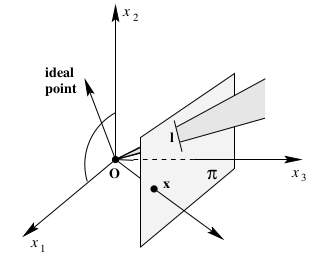
\includegraphics[width=0.45\textwidth]{pictures/02_projective_pane_model.png}
  \caption[Die Kameraprojektion]{Punkte und Linien in $\mathbb{P}^2$ aus $\mathbb{P}^3$ (Hartley, 2003 \cite{Hartley:MVG})}
\end{figure}
Das Abbilden von 3-D auf 2-D ist eine Projektion die durch eine Zentralprojektion beschrieben wird. Die Strahlen von allen Punkten laufen durch das Projektionszentrum, in diesem Fall der Brennpunkt. Der Brennpunkt ist gleichzeitig das Kamerazentrum. Dabei schneiden die Strahlen die Bildebene, die vor der Kamera aufgespannt wird. Die Schnittpunkte sind die Bildpunkte. Dieses Modell entspricht dem Modell der Lochbildkamera. D.h. Fokus und Linsenstärke werden vernachlässigt. 

In der projektiven Geometrie ist die Zentralprojektion eine Abbildung von $\mathbb{P}^3$ zu $\mathbb{P}^2$. Ein Punkt in  $\mathbb{P}^3$ kann als $(X, Y, Z, T)^T$ in homogenen Koordinaten geschrieben werden und das Projektionszentrum als $(0, 0, 0, 1)^T$. Um $\mathbb{P}^3$ auf $\mathbb{P}^2$ ab zu bilden kann die sogenannte Kameramatrix (oder Projektionsmatrix) P verwendet werden.\cite{Hartley:MVG} Es ergibt sich eine lineare Abbildung zwischen Kameraprojektion und einem Punkt im Raum als 

\begin{equation}
  \begin{pmatrix}
    x\\ y \\ w
  \end{pmatrix}
  = P_{3\times4}
  \begin{pmatrix}
    X\\Y\\Z\\T
  \end{pmatrix}
\end{equation}



%%%%%%%%%%%%%%%%%%%%%%%%%%%%%%%%%%%%%%%%%%%%%%%%%%%%%%%%%%%%%%%%%%%%%%%%%%%%%%%
\subsection{Korrespondenzanalyse}
Bildkorrespondenzen sind Merkmale in Bildern die das selbe Objekt in zwei unterschiedlichen Bildern beschreiben und als Ankerpunkte zwischen den Kamerapositionen dienen. Wenn eine Rekonstruktion von 3-D Punkten durchgeführt werden soll muss immer die Aufgabe der Bestimmung von Korrespondenzen gelöst werden.


Bei der Korrespondenzanalyse geht es ganz allgemein darum übereinstimmende Bildmerkmale in zwei Bildern zu finden. Handelt es sich um zwei Bilder einer Stereokamera, spezifiziert sich die Aufgabenstellung zur Stereoanalyse.

Die Korrespondenzanalyse ist aus dem Anwendungsgebiet der Bewegungsschätzung für Videostreaming hervorgegangen. Korrespondenzanalyse wird in der Videokodierung genutzt um zu Schätzen, in welchen Bereichen eines Bildes Bewegung stattgefunden hat. Für die Bereiche werden Bewegungsvektoren erstellt. Bilder werden anschlie{\ss}end mit den Bewegungsvektoren kodiert und so müssen nur Teile des Bildes übertragen und aktualisiert werden. \cite{stereoSchreer}  

Bei SfM und Visueller Odometrie soll im Grunde genau das Gegenteil erreicht werden. Die Szene ist überwiegend statisch und die Bewegung der Kamera muss geschätzt werden. Schwierigkeiten, die bei der Korrespondenzanalyse auftreten, sind beispielsweise Regionen die nur im Bildfeld einer Kamera vorhanden sind, aufgrund von Geometrie oder Verdeckung, wiederkehrende Muster oder Oberflächen mit schwacher Textur.
\newline

Die Korrespondenzanalyse kann in pixelbasierte und merkmalsbasierte Verfahren unterschieden werden. Für das erstellen der Disparitätenkarte (ein Schritt zur Ermittlung der Tiefenwerte von Pixeln) wird eine pixelbasierte Stereoanalyse verwendet. Zum einen, da eine hohe Informationsdichte benötigt wird. Zum anderen kann aus der Kenntnisse über die Geometrie des Stereoaufbaus die Suche auf einen eindimensionalen Suchraum beschränkt werden. Diese Aussage wird in der folgenden Betrachtung der Epipolargeometrie noch ersichtlich.
\newline

Für die Korrespondenzanalyse der Bewegungsschätzung werden merkmalsbasierte Verfahren angewendet.

%%%%%%%%%%%%%%%%%%%%%%%%%%%%%%%%%%%%%%%%%%%%%%%%%%%%%%%
\subsection{Verbinden von zwei Ansichten durch Epipolargeometrie}
\begin{center}
    \begin{figure}[!h]
      \centering
      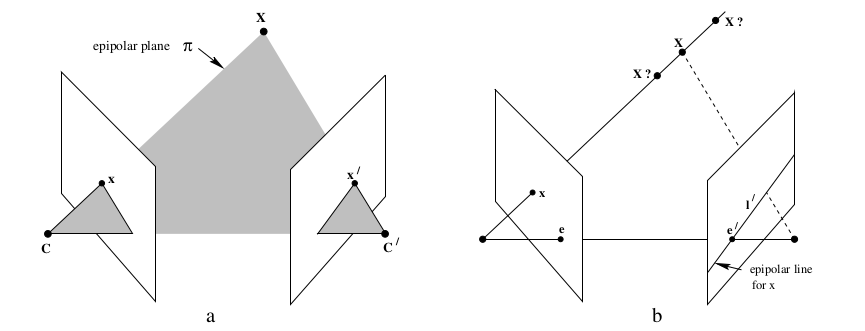
\includegraphics[width=\textwidth]{pictures/epipane_01.png}
      \caption[Bildebenen mit Epipolarlinien]{(a) Die Kameras sind gekennzeichnet als $C$ und $C'$, vor Ihnen spannen sich die jeweiligen Bildebenen auf. 
      (b) X muss auf seiner Epipolarlinie liegen. (Hartley, 2003 \cite{Hartley:MVG})}
      \label{fig:epigem1}
    \end{figure}
\end{center}

Die Epipolargeometrie besagt, dass die Kamerazentren $C$ und $C'$, die Bildpunkte $x$ und $x'$ und die Raumpunkte koplanar sein müssen.
%
\begin{equation}
  Cx\cdot(C C' \times C x') = 0
  \label{eq:epi_const}
\end{equation}

Diese Forderung wird durch die Fundamentalmatrix $F$ abgebildet. Die Fundamentalmatrix wird als algebraische Repräsentation der Epipolargeometrie bezeichnet. Sie ist eine homogene $3 \times 3$ Matrix mit Rang(2), die nachfolgende Gleichung erfüllt \cite{Hartley:MVG} 

\begin{equation}
  {x'}^{T}Fx = 0
  \label{eq:fun}
\end{equation}

%
In Matrixschreibweise mit Homogenen Koordinaten lässt sich \ref{eq:fun} schreiben als

\begin{equation}
  \begin{bmatrix}
    {x_R}_i & {y_R}_i & 1
  \end{bmatrix}
  \begin{bmatrix}
    f_{11} & f_{12} & f_{13} \\
    f_{21} & f_{22} & f_{23} \\
    f_{31} & f_{32} & f_{33} \\
  \end{bmatrix}
  \begin{bmatrix}
    x_i \\
    y_i \\
    1
  \end{bmatrix}
  = 0
\end{equation}

Zwischen diesen koplanaren Punkten lässt sich eine Ebene aufspannen. Diese Ebene wird als Epipolarebene bezeichnet. Jede Kamera spannt au{\ss}erdem eine Bildebene in Blickrichtung auf. Die Epipolarebene schneidet die Bildebenen. Aus Sicht der ersten Kameraposition befindet sich $X$ auf einem Strahl der vom Projektionszentrum durch den Bildpunkt $x$ der Bildebene läuft. Dieser Strahl entspricht der Epipolarlinie im zweiten Bild, die durch die Epipolarebene geschnitten wird.
%%
%
Um einen Punkt eindeutig bestimmen zu können, lässt sich folgende Beschränkung einführen: $x'$ muss auf seiner Epipolarlinie $l'$ liegen um eine Projektion des Gleichen Punktes $X$ zu sein wie $x$.
\begin{equation}
  x \mapsto l' 
\end{equation}
Die Epipolarlinie ist die Überschneidung zwischen Epipolar- und Bildebene. Der Epipol ist der Punkt in der Bildebene in welchem diese die Basislinie schneidet. Die Baseline ist die Gerade die zwischen den Kamerazentren $C$ und $C'$ gezogen werden kann. 

%%%%%%%%%%%%%%%%%%%%%%%%%%%%%%%%%%%%%%%%%%%%%%%%
\subsection{Sonderfall Stereo Vision}
\begin{center}
    \begin{figure}[h!]
    	\centering
    	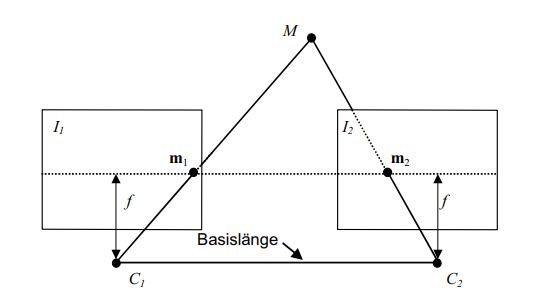
\includegraphics[width=.75\textwidth]{02_stereo.png}
    	\caption[Parallele Epipolarlinien]{Sind die Kamerazentren exakt parallel, verlaufen die Epipolarlinien parallel zur Baseline, (Schreer, 2005 \cite{stereoSchreer})}
    	\label{fig:stereoepi}
    \end{figure}
\end{center}

Bei einem Stereo Kamera Aufbau wird von einem Sonderfall der Epipolargeometrie nutzen gemacht. Die Kamerazentren sind dabei exakt parallel zueinander ausgerichtet. Das führt dazu, dass die Epipole ins Unendlichen verschoben werden. Sind $C$ und $C'$ parallel, verlaufen die Epipolarlinien $l$ und $l'$ parallel zur Baseline. Das besondere daran ist, das nun die Epipolargeometrie für jeden Punkt $x'$ sofort bekannt ist. Die Forderung für $x'$ ist $x' \mapsto l'$ und genauso gilt $x \mapsto l$. $l$ und $l'$ liegen nun auf gleicher Höhe. Damit ist $l'$ aus $l$ bekannt.
\newline

Die Bestimmung von $x'$ wird auf diese Art wesentlich beschleunigt. Dieser Umstand lässt sich nicht für aufeinanderfolgende Bilder $I$ und $I'$ ausnutzen. Stattdessen wird die Geometrie beim erstellen der Tiefenkarte verwendet. Dazu wird das aktuelle Bildpaar, welches zeitgleich aus der gleichen Fahrzeugpose aufgenommen untersucht.
\newline 

Prinzipiell wird dabei für jedes Pixel wie folgt vorgegangen:

Zuerst wird die Epipolarlinie gesucht. 

Anschlie{\ss}end wird die Linie nach der besten Übereinstimmung abgesucht.

Schlie{\ss}lich wird die Tiefe aus der Verschiebung berechnet

\begin{equation}
  Z = \frac{bf}{d}
\end{equation}
%%%%%%%%%%%%%%%%%%%%%%%%%%%%%%%%%%%%%%%%%%%%%%%%%%%%%%%%%%%%%%%%%%%%%%%%%%%%%%%%%%
%%%%%%%%%%%%%%%%%%%%%%%%%%%%%%%%%%%%%%%%%%%%%%%%%%%%%%%%%%%%%%\section{Visuelle Verfahren für Lokalisierung}
\subsection{Structure From Motion - SfM}
Um die Pose einer Kamera bestimmen zu können, muss die Positionen der Bildpunkte in der Umgebung bekannt sein. Ein Verfahren zur Rekonstruktion von 3-D Objekten aus Bildern ist als Structure from Motion (SfM) bekannt. Visuelle Odometrie  zählt als Sonderfall von SfM.
\newline

SfM ist rechenaufwendig und wird überwiegend offline betrieben. Anders als Visuelle Odometrie, die immer online betrieben wird. Offline bedeutet hier, dass eine Menge an Bildern (geordnet oder ungeordnet) bereits vollständig vorliegt. Viele Algorithmen die heute für Visuelle Odometrie oder SLAM eingesetzt wurden sind bereits seid den 80er Jahren bekannt wo sie für SfM entwickelt wurden. \cite{LonguetHiggins1981ACA}
\newline

SfM hat viele interessante Anwendungsgebiete, wie in der Geoinformatik und Informationsgewinnung aus offline Bilddaten. Beispielsweise veröffentlichten Sameer Agarwal et. al. 2009 das Paper \"Building Rome in a Day\" indem sie zeigten wie eine 3-D-Rekonstruktion der Stadt Rom in 21 Stunden angefertigt wurde. Als Eingangsdaten verwendeten sie ausschlie{\ss}lich die Bilder, die bei der Suche für das Schlagwort \"Rom\" von der Photo-Community Plattform Flickr ausgegeben wurden.\cite{RomeDay}

\subsection{Simultaneous Localization and Mapping - SLAM}
\begin{center}
  \begin{figure}[h!]
    \centering
    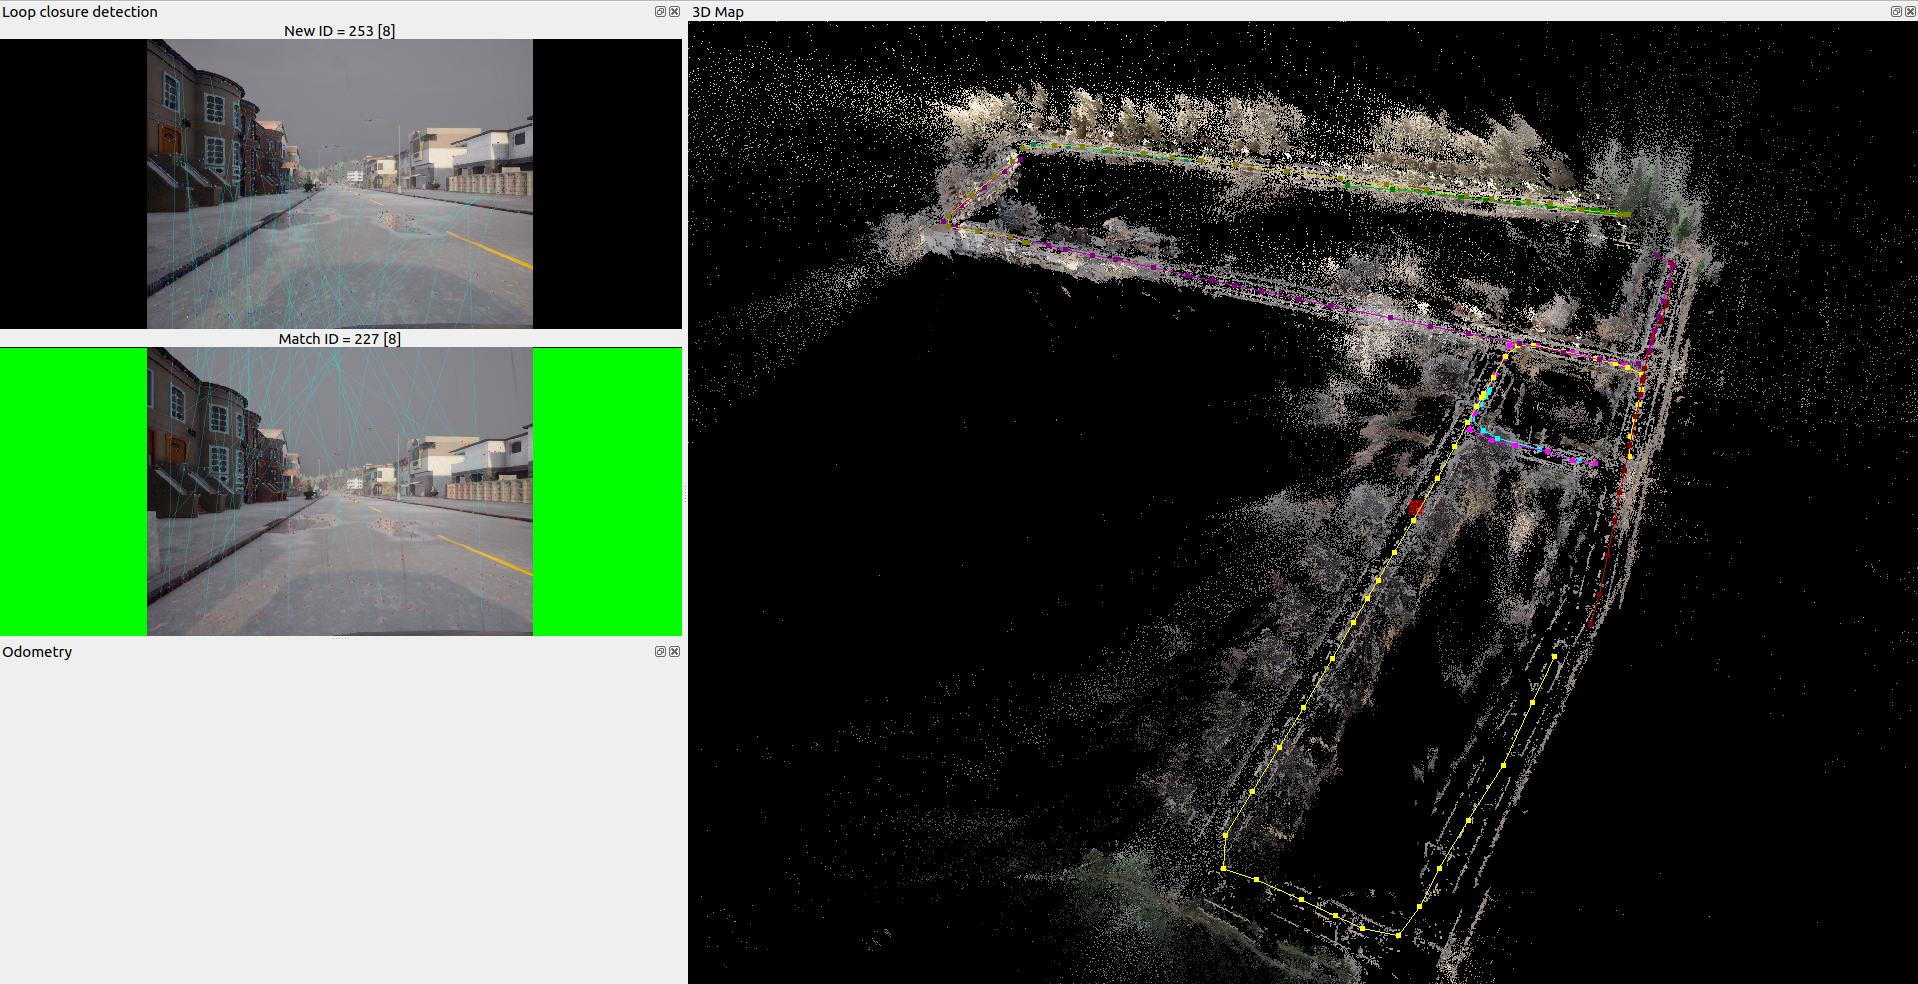
\includegraphics[width=\textwidth]{pictures/Screenshot from 2022-02-19 21-49-24.png}
    \caption[SLAM Map aus CARLA Testfahrt]{Screenshot einer SLAM Karte einer CARLA Testfahrt. Die Karte wurde mit dem Visual Odometrie System der Abschlussarbeit durch Erweiterung mit RTAB SLAM erzeugt.}
    \label{fig:rtabslam}
  \end{figure}
\end{center}
Eine andere Kategorie von SfM ist Simultaneous Localization and Mapping (SLAM). Hier wird neben der Lokalisierung gleichzeitig eine Umgebungskarte erstellt. Die Karte ergibt sich aus den 3-D Punkten, die aus den Merkmalen der Bildpaare rekonstruiert wurden. Während diese Punkt für die Visuelle Odometrie nach der Schätzung verworfen werden, fasst SLAM sie zu 3-D Punktwolken zusammen. Diese Punktwolken bilden eine Karte der Umgebung.
\newline

Im Gegensatz zu SfM wird SLAM i.d.R. online also in Real-Time betrieben. Bei VO und SLAM werden die Eingangsbilder sequentiell akquiriert und die Pose von einem Zeitschritt zum nächsten geschätzt.
\newline

Auch SLAM Schätzt die zurückgelegt Trajektorie. Die erstellte Umgebungskarte wird genutzt um ein sog. Loop-Closure zu entdecken. Loop-Closure bedeutet, dass zuvor detektierte Landmarken wiedererkannt werden. Der Agent kann also feststellen, das er sich zuvor bereits in der Nähe der aktuellen Position befunden hat.

Die bisherigen Schätzungen werden bei SLAM als Graph gespeichert. Die Posen sind Knoten. So entsteht ein Pose Graph. Nach erneutem Besuchen einer Landmarke kann eine Pose Graph Optimierung ausgeführt werden, bei dem die Positionen aller Knoten rekursiv an die korrigierte Schätzung angepasst werden.

\subsection{Verschiedene Ansätze für Visuelle Odometrie}
Das Konzept der Visuellen Odometrie wurde zuerst 1980 als Lokalisierung für Mars Rover eingeführt und erfolgreich umgesetzt. Ein Gro{\ss}teil der Anfänglichen Forschung kam daher aus der Raumfahrt. Die Motivation Visuelle Odometrie für Marsrover einzusetzen liegt vor allem in der Abwesenheit von GNSS und dem extrem unebenen Untergrund. Anwendungen für VO und SLAM Implementierungen lassen sich heute in den unterschiedlichsten Bereichen finden und haben einen festen Platz in der Erforschung autonomer Fahrzeuge.
\newline

% \subsubsection{Problemstellung}
\begin{center}
    \begin{figure}[h!]
    	\centering
    	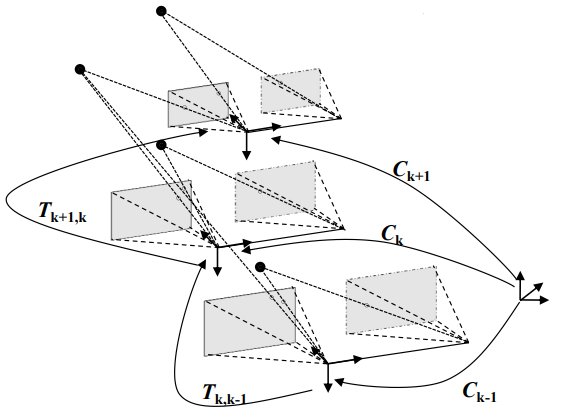
\includegraphics[width=.75\textwidth]{02_VO_scaramuzza.png}
    	\caption[Visuelle Odometrie Problemstellung]{Illustration der Visuelle Odometrie Problemstellung. Ein Kamerakoordinatensystem $C_{k}$ bewegt sich in Bezug zum Weltkoordinatensystem. Zu diskreten Zeitpunkten $k$ soll die Transformationsmatrix $T_{k}$ zwischen den Kameraposen $C_{k}$ geschätzt werden. (Scaramuzza, 2011 \cite{ScFrVO})}
    	\label{fig:voproblem}
    \end{figure}
\end{center}
Um die Problemstellung der Visuellen Odometrie zu erläutern wird angenommen, dass sich zwei Kameras als Stereokamerasystem auf einem autonomen Fahrzeug befinden. Es werden zwei Koordinatensysteme betrachtet; das lokale Kamerakoordinatensystem $C$ und das globale Weltkoordinatensystem. Dabei ist $C$ der gemeinsame Koordinatenursprung beider Kameras und befindet sich im Brennpunkt der linken Kamera.

Um die Kameraposen über einen Verlauf, mit diskreten Zeitabständen $k$, zu schätzen, wird zunächst die Transformation $T_{k,k-1}$ zwischen der vorherigen Position $C_{k-1}$ und der aktuellen Pose $C_{k}$ geschätzt.


Durch addieren von Transformation $T_{k,k-1}$ auf die vorherige Pose $C_{k-1}$ ergibt sich so die aktuelle geschätzte Kameraposition $C_{k}$.

Daraus folgt, dass ein Aneinanderreihen aller Transformationen aus der Initialpose $k = 0$, heraus die geschätzte Trajektorie der Kamera beschreibt.

%%
\begin{equation}
\label{eq:tmatrix2}
T_{k,k-1} = 
    \begin{pmatrix}
    R_{k,k-1} & t_{k,-1}\\
    0 & 1
    \end{pmatrix}
\end{equation}
%%
Wie die Gleichung \ref{eq:tmatrix} zeigt, setzt sich die Transformationsmatrix $T \in \mathbb{R}^{4x4}$ aus einer Rotationsmatrix $R \in \mathbb{R}^{3x3}$ und einem Translationsvektor $t \in \mathbb{R}^{3x1}$ zusammen. $T$ ist also der Ergebnisvektor einer einzelnen Odometrieschätzung.
\newline

Der zurückgelegt Pfad wird inkrementell geschätzt. Anders als bei SLAM gibt es keine Korrektur über einen längeren Zeitraum, weshalb die Drift über die Zeit akkumuliert. Wird VO als Front-End für (V-)SLAM implementiert kann die Drift durch Loop-Closure korrigiert werden. Eine andere Möglichkeit der Korrektur, ist über  Sensorfusion mit anderen Sensoren. Im Laufe des letzten Jahrzehnts sind dabei überwiegend Forschungsergebnisse zum Einsatz von Visual-Inertial-Odemetry (VIO)veröffentlicht worden.

Im Allgemeinen zeigt VO weniger Drift als klassische odometrische Messverfahren durch Radsensoren, Drehgeber oder Gyroskop.\cite{ScFrVO}

Für einen VO Algorithmus kann zwischen Feature Based, Appearance Based und Lernenden Verfahren unterschieden werden. 

\subsubsection{Feature-based Algorithmen}
Beim Feature based oder merkmalsbasierten Ansatz werden markante Merkmale gefunden und von Frame zu Frame verfolgt. Feature Based Algorithmen durchlaufen immer zwei Phasen: Zuerst werden Merkmale in aufeinanderfolgenden Bildern gefunden. Anschlie{\ss}end werden die Merkmale abgeglichen um übereinstimmende Merkmale zu bestimmen.


Jeder der Phasen hat seine Herausforderungen. Für eine zuverlässige Merkmalsdetektion werden Merkmalsdetektoren berechnet. 

Der zweite Schritt ist für das Problem der Korrespondenzfindung bekannt. Veränderungen in den Bildern wie Bewegung, Verdeckung oder Veränderung der Skalierung machen die Korrespondenzanalyse zu einer anspruchsvollen Aufgabe. 

Wurden Korrespondenzen zwischen den Bildern bestimmt, wird die Pose aus der Minimierung des Reprojektionsfehlers zwischen den Bildern bestimmt. 
%
\subsubsection{Appearance-based Algorithmen}
Appearance-based Methoden kommen gänzlich ohne Merkmalsdetektion und Matching aus. Stattdessen werden die Intensitätswerte aller Pixel analysiert und zwischen zwei Bildern auf das gesamte Bild untersucht. Anstelle der Minimierung des Reprojektionsfehlers wird ein sog. Photometrische Fehler minimiert.


Appearance-based Methoden liefern aufgrund der gro{\ss}en Informationsmenge die aus den Bildern genutzt wird sehr gute Ergebnisse, sind aber extrem rechenaufwendig. Daher wurden sie für mobile Systeme erst vermehrt im vergangenen Jahren, aufgrund leistungsfähiger Hardware, untersucht.

\subsubsection{Lernende Verfahren}

Die Erforschung von Visuelle Odometrie mit lernenden Verfahren ist vor allem für monokulare Visuelle Odometrie von Bedeutung. Hier fehlt die Skaleninformation für die Berechnung der 3-D Punkte bzw der Tiefeninformation und muss zusätzlich geschätzt werden. Ein Möglicher Deep Learning Ansatz wäre Beispielsweise, ein Neuronales Netz zuerst mit Videos eines Stereo VO Systems zu trainieren um es dann in Mono Setups einzusetzen. Versucht wurde dies bei D3VO der Technischen Universität München. \cite{yang2018dvso}
\newline

Bisher erzielen traditionelle Methoden nach wie vor bessere Ergebnisse, als Deep Learning Ansätze. Es wird aktuell viel auf diesem Gebiet geforscht. Sobald die richtige Methodik gefunden wird könnten die monokularen VO Systeme mit neuronalen Netzen die traditionellen Stereo Systeme ablösen, da sie weniger Hardware benötigten.  

\chapter{Extraktion von Bildmerkmalen}
\label{ch:merkmale}
Das Extrahieren von Bildmerkmalen ist zentraler Bestandteil aller Feature-based Algorithmen. Es muss festgelegt werden, welcher Typ von Merkmal gefunden werden soll, ein Suchalgorithmus ausgewählt werden und schlie{\ss}lich Überlegt werden durch welchen Deskriptor die Merkmale Beschrieben werden sollen.
%%%%%%%%%%%%%%%%%%%%%%%%%%%%%%%%%%%%%%%%%%%%%%%%%%%%%%%%%%%%%
\section{Auffinden von Merkmalen}
\subsection{Merkmale Beschreiben durch Nachbarschaftsoperationen}
% LINK SOURCE https://cmsc426.github.io/pano-prereq/
Merkmale sind lokale Punkte im Bild die durch die Pixel in ihrer Nachbarschaft charakterisiert sind. Gute Merkmale sind möglichst eindeutig bestimmbar und lassen sich nicht mit anderen Stellen im Bild verwechseln. Anwendungen wie Structure from Motion setzen Merkmale voraus, die sich auch nach Veränderungen des Bilds wie beispielsweise durch Translation, Rotation oder Lichtverhältnisse wiedererkennen lassen. Um diesen Anforderungen gerecht zu werden, eignen sich die Interest-Operatoren (auch Interest-Points, Corner).

Es sollen zunächst einige allgemeine Grundlagen zur Merkmalsdetektion betrachtet werden. Es wird einführend auf Kantendetektion eingegangen um von dort zu den Interest-Operatoren zu kommen.
\newline

Eine einfache Operation durch die Merkmale gefunden werden können, ist die Faltung.

\begin{equation}
  (f*g)(t) = \int_{-\infty}^{\infty} f(\tau)g(t-\tau)d\tau = \int_{-\infty}^{\infty} f(t-\tau)g(\tau)d\tau
  \label{eq:convolution}
\end{equation}

Dabei ist $g$ der Faltungskern (auch Kernel oder Filter) und bestimmt welche Operation auf das Bild angewandt wird. Durch den Kern kann ein Bild beispielsweise geglättet, schärfer gemacht werden oder Kanten extrahiert werden.

Faltunsgkerne lassen sich au{\ss}erdem als Approximation verwenden, wenn eine Ableitung des Bildes gebildet werden soll. Die Ableitung eines Bildes ist essentiell für die Bildverarbeitung, da sie den Gradient bildet. Durch die Bestimmung der Gradienten können Kanten und ihre Eigenschaften beschrieben werden. Der Gradientenvektor ist definiert als

\begin{equation}
  \nabla f=\left[\dfrac{\delta f}{\delta x}, \dfrac{\delta f}{\delta y}\right]
\end{equation}

Der Gradient eines Bildes zeigt in die Richtung, in der es die grö{\ss}te Veränderung der Intensitätswerte der Pixel gab. Daher lässt sich die Richtung der grö{\ss}ten Veränderung bestimmen durch

\begin{equation}
  \theta=tan^{-1}\left(\dfrac{\delta f}{\delta y}\Bigg{/}\dfrac{\delta f}{\delta x}\right)
\end{equation}

Die Richtung verläuft immer Senkrecht zur Kante. Die Stärke des Anstiegs und damit die Stärke der Kante und ist gegeben durch den Betrag des Gradienten

\begin{equation}
  ||\nabla f|| = \sqrt{\left(\dfrac{\delta f}{\delta x}\right)^2 +
  \left(\dfrac{\delta f}{\delta y}\right)^2}
\end{equation}

Für die Bildverarbeitung können die Partiellen Ableitungen praktisch berechnet werden als 

\begin{equation}
  \begin{split}
  \delta x &= f(x+1,y) -  f(x,y)\\
  \delta y &= f(x,y+1) -  f(x,y)
  \end{split}
\end{equation}

Beispiele für bekannte Kanten Operatoren sind der Sobel Operatior, Prewitt, Roberts, Laplacian of Gaussian (LoG) und Canny.

\begin{equation}
  \rho(\tau)= K\int_{-\infty}^\infty x(t) m(t + \tau) {\rm d}t
\end{equation}
Die gesuchten Interest-Operatoren entstehen durch das aufeinandertreffen zweier Kanten. Das bedeutet in der Nachbarschaft dieses Punktes existieren zwei starke und unterschiedliche Gradientenanstiege. Die einfachste Art Interest-Points zu detektieren ist durch Korrelation.

\subsection{Algorithmen zum Auffinden von Interest-Operatoren}
Für die Lokalisierung werden Detektoren verwendet, die nach Interest-Operatoren im Bild suchen. Interest-Punkte haben gegenüber Punkten und Kanten die entscheidende Eigenschaft invariant gegenüber Veränderungen in Rotation, Skalierung und Lichtverhältnissen zu sein.
 
\subsubsection{Moravec-Operator}
Der Moravec-Operator wurde 1977 veröffentlicht. Berechnet die mittlere quadratische Gradientensumme und bestimmt Ecken anhand eines Schwellwertes. Der Moravec-Operator eignet sich nicht im Kontext von Lokalisierung, da er nicht Rotationsinvariant ist.

\subsubsection{Harris Corner Detektor}
\begin{figure}[!h]
  \centering
    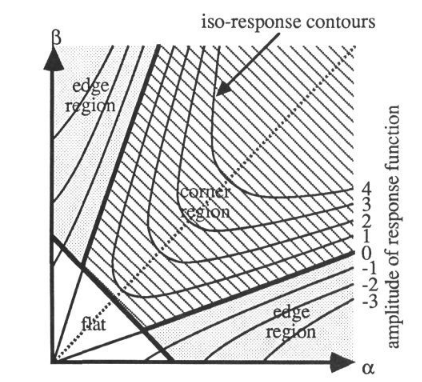
\includegraphics[width=0.4\linewidth]{harris_autocorrelation.png}
    \caption[Harris Interest-Operator Detektor]{Klassifikation der Autokorrelation in Edge, Flat und Corner Region. $\alpha$  und $\beta$ entsprechen $\lambda_1$ und $\lambda_2$ (Harris, 1988 \cite{Harris88alvey.Ha})}
\end{figure} 

Der Harris Corner Detektor wurde 1988 basierend auf dem Moravec-Operator veröffentlicht. Der wesentliche Unterschied ist, dass Harris eine Rotations- und Skalierungsinvarianz durch integration von Autokorrelation erreicht. 
Auf einen Bildpunkt angewandt kann durch eine Funktion $E(u,v)$ die Veränderung der Intensitätswerte für eine Verschiebung eine Punktes in jede Richtungen gefunden werden.

% Windows Funktion: Box oder Gaussian
\begin{equ}[!ht]
  \begin{equation}
    E(u,v) = \sum_{x,y} \underbrace{w(x,y)}_{\text{Window Fkt}} [\underbrace{[I(x+u, y+v)}_{\text{verschobene Intensität}} - \underbrace{I(x,y) ]^2}_{\text{Original Intensität}}
  \end{equation}
  \caption{Formel des Harris-Corner Detektors}
\end{equ}

Für die Detektion von Interest-Operatoren muss die Funktion maximiert werden.
Verwendung der Taylor Approximation 1. Grades führt zu nachfolgenden Schritten. 

%
\begin{equation}[!ht]
  f(x+u, y+v) \approx f(x,y) + uf_{x}(x,y) + vf_{y}(x,y)
\end{equation}
\begin{equation}
  \begin{aligned}
    E(u,v) &= \sum \left[ I(x+u, y+v) - I(x,y) \right]^2 \\
    &= \sum \left[ I(x,y) + uI_{x} + vI_{y} - I(x,y) \right]^2 \\
    &= \sum u^2I_{x}^2 + 2uvI_{x}I_{y}-v^2I_y^2\\
    &= \sum \begin{bmatrix} u & v \end{bmatrix} 
    \begin{bmatrix} I_x^2 & I_xI_y \\ I_xI_y & I_y^2 \end{bmatrix} 
    \begin{bmatrix}u \\v \end{bmatrix} \\
    &= \begin{bmatrix} u & v \end{bmatrix} \left(\sum 
    \begin{bmatrix} I_x^2 & I_xI_y \\ I_xI_y & I_y^2 \end{bmatrix} 
    \right) \begin{bmatrix}u \\v \end{bmatrix} 
  \end{aligned}
\end{equation}

Für kleine Verschiebungen ergibt sich die bilineare Approximation

\begin{equation}
  E(u,v) \cong \begin{bmatrix}
    u,v
  \end{bmatrix} M \begin{bmatrix}
    u\\ v
  \end{bmatrix}
\end{equation}

Mit M als

\begin{equation}
  M = \sum_{x,y} w(x,y)  
  \begin{bmatrix} I_x^2 & I_xI_y \\ I_xI_y & I_y^2 \end{bmatrix}  
\end{equation}

Der zweite Part des Harris Operators ist die Score Funktion.

\begin{equation}
  R = \lambda_1 \lambda_2 - k(\lambda_1 + \lambda_2)^2 = \det(M) - k(\operatorname{trace}(M))^2
\end{equation}

Durch den Score wird überprüft, ob das Fenster einen Interest-Operator enthält. 

\subsubsection{Shi-Tomasi Detektor (GFFT)}
\begin{figure}[!ht]
  \centering
  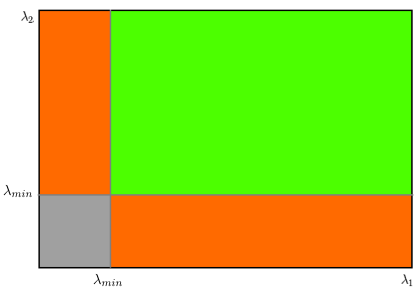
\includegraphics[width=0.45\textwidth]{pictures/03_shitomasi_space.png}
  \caption[GFTT Detektor Merkmalsfindung]{Ein Merkmal wird bei GFTT durch eine Min-Funktion bestimmt. Nur wenn $\lambda_1$ und $\lambda_2$ über dem Grenzwert $\lambda_{min}$ liegen, handelt es sich um einen Interest-Operator (grüner Bereich) (OpenCV Docs GFTT, 2022)}
\end{figure}

Das erste mal würde dieser Detektor 1994 unter dem Titel \textit{Good Features To Track} in einem Paper veröffentlicht. Daher wird er sowohl als Shi-Tomasi als auch GFTT Detektor bezeichnet. Dieser Detektor ist gleich dem Harris Detektor mit Ausnahme einer Änderung im Scoring. Statt das Scoring über die Eigenwerten zu berechnen, wurde vorgeschlagen, die Score direkt aus einer Min-Funktion der Eigenwerte zu setzen. 

\begin{equation}
  R = min(\lambda_1,\lambda_2)
\end{equation}

Dadurch kann die Ursprünglich eingeführte Funktion weggelassen werden.

\subsubsection{FAST}
Features from Accelerated Segment Test (FAST) wurde 2006 veröffentlicht. FAST ist für seine Geschwindigkeit bekannt. Anwendungen wie SLAM haben sehr hohe Anforderungen an die Laufzeit der Merkmalsdetektoren. FAST hat eine kürzere Rechenzeit als die vorangegangenen Detektoren und wurde speziell für den Einsatz in zeitkritischen Anwendungen entwickelt.

\begin{figure}[!ht]
  \centering
  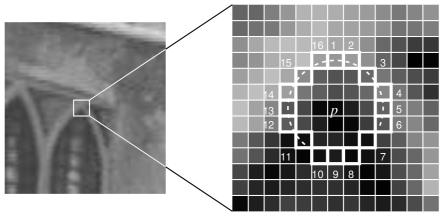
\includegraphics[width=0.75\textwidth]{pictures/03_fast_speedtest.jpg}
  \caption[FAST Detektor Speedtest]{FAST Detektor Performance Test, (E. Rosten and R. Porter and T. Drummond, 2010 \cite{FAST})}
\end{figure}

FAST legt einen Kreis von 16 Pixel um ein interessantes Pixel q. Der Kreis wird durchnummeriert und der Intensitätswert $Iq$ von q erfasst. Es wird Verglichen ob im Kreis N zusammenhängende Pixel heller als $I_q+thresh$ oder dunkler als $I_q-tresh$ sind. Wobei $thresh$ ein Grenzwert ist.\newline

Nun werden nicht alle 16 Pixel untersucht. FAST schlägt einen High-Speed-Test vor bei dem nur 4 Pixel getestet werden. Zuerst werden die Intensitäten von 1 und 9 gegen den Grenzwert getestet, dann 5 und 13. Ist p ein Interest-Punkt müssen mindestens 3 dieser Pixel heller as $I_q + thresh$ oder dunkler als $I_q - tresh$ sein.\newline

Das Verfahren ist tatsächlich sehr schnell, wei{\ss}t aber einige Mängel auf. Die Empfehlung ist eine Kombination mit einem Machine Learning Ansatz, dadurch können die Nachteile gut behoben werden. \cite{cvdocFAST} Für den Systementwurf wurden generell nur direkte Verfahren ohne Machine Learning ausgewählt und anstatt des FAST Detektors daher der GFTT (Shi-Tomasi Detektor) Detektor eingesetzt.


%
\pagebreak
%%%%%%%%%%%%%%%%%%%%%%%%%%%%%%%%%%%%%%%%%%%%%%%%%%%%%%%%%%%%%
\section{Matching}
Beim Feature Matching wird festgestellt, ob es sich bei Merkmalen die in zwei verschiedenen Bildern gefunden wurden um das selbe Merkmal handelt. Hierzu wird für jedes Merkmal des ersten Bildes in dessen ursprünglichen Position im zweiten Bild gesucht. Wie gro{\ss} die Suchumgebung um die ursprüngliche Position herum ist, hängt von der gewählten Abstandsmetrik des Suchalgorithmus ab.
\newline

Generell hängt die Leistung der Matchingverfahren von den Eigenschaften der zugrunde liegenden Merkmale als auch von der Wahl der zugeordneten Bilddeskriptoren ab. Es ist daher wichtig die geeigneten Detektoren und Deskriptoren auszuwählen. Beispielsweise wäre für ein Mikroskop Bild einer organischen Struktur ein Blob-Detektor wahrscheinlich am besten geeignet, währen in einer Urbanen Umgebung mit menschengemachten, geometrischen Strukturen ein Interest-Operator wesentlich erfolgversprechender ist.
\newline

\subsection{Übereinstimmungen finden}
Zwischen zwei Bildern sollen gemeinsame Merkmale gefunden werden. Aus gefundenen Merkmalen besitzt jedes Bild eine eigene Menge von Merkmalsdeskriptoren. Jeder Deskriptor befindet sich an einer bestimmten Stelle im Bild. Für das Matching wird ein Deskriptor des ersten Bildes nicht mit der gesamten Menge an Deskriptoren des zweiten Bildes verglichen. Stattdessen wird um die Position, an der sich der Deskriptors im ersten Bild befindet, eine Region of Interest bzw Suchfenster gebildet. Es werden dann nur Deskriptoren des zweiten Bildes für den Abgleich herangezogen, die innerhalb dieser Region auftreten. Selbst beim, von OpenCV implementierten, Brute Force Matching wird in einem bestimmten Abstand zum gesuchten Deskriptor gesucht. 

\begin{equation}
    \begin{aligned}
      d_{euclidean}(p,q) & = \Vert q-p {\Vert}_2&\\
      & = \sqrt{(q_1 - p_1)^2 + ... + (q_n - p_n)^2}&\\
      & = \sqrt{\sum_{i = 1}^{n} (q_i - p_i)^2  } 
      \label{eq:l2norm}
    \end{aligned}
\end{equation}

Die Grö{\ss}e des Suchfensters wird über den Abstand angegeben. Bei klassischen Deskriptoren wie SIFT und SURF wird im Euklidischen Abstand gesucht. Bei Binär-Deskriptoren wie ORB und BRISK sollte der Hamming-Abstand verwendet werden.   

\begin{equation}
  d_{hamming} \left ( q,p \right ) = \sum_{i=0}^{n-1} \left ( q_i \oplus p_i \right )
  \label{eq:hamming}
\end{equation}

Dei Begründung liegt in der unterschiedlichen Beschaffenheit der Deskriptoren. Bei SIFT repräsentieren sie Histogramme von gerichteten Gradienten. Bei ORB handelt es sich um Binärwörter die durch den XOR-Operator verglichen werden können wie in Gleichung \ref{eq:hamming} zu sehen. 

\subsection{Matching Ergebnisse Filtern}
Die Matches die durch die Suche bestimmt wurden sind teilweise nur sich stark ähnelnde Merkmale und keine echten Übereinstimmungen. Die Ergebnisse sind also von unterschiedlicher Qualität. Sie müssen daher noch gefiltert werden. Zum einen wird so bei den folge Schritten Zeit gespart. Zum anderen handelt es sich im Grunde um Ausrei{\ss}ern die ohne Filterung zu Fehlern in nachfolgenden Schätzungen führen werden.

Um die Ergebnisse zu Filtern gibt es drei Unterschiedliche Ansätze:

\begin{description}
  \item[Lowes Distance Ratio Test] Der Test überprüft ob es in der direkten Nachbarschaft, weitere Matches gibt. Falls ja und das Match hat einen Ratio nahe eins, sind das Match und sein Nachbar von gleicher Qualität. Bei dem Ausgewählten Match handelt es sich dann mit 50\% Wahrscheinlichkeit um einen Ausrei{\ss}er. Daher werden beide Matches verworfen. Der Ratio unter dem die Merkmale liegen müssen ist variabel und wird über einen threshold and die Funktion übergeben. \cite{Lowe04distinctiveimage} 
  \item[Cross Check] Beim Cross-Check werden die Resultate der beiden Bilder darauf Verglichen, ob das beste Match in Set A auch das beste Match in Set B war und umgekehrt. Cross Checking kann beim Brute Force Matcher verwendet werden. 
  \item[Geometrischer Test] Ausgleichsverfahren basierend auf der Methode der kleinsten Quadrate wie beispielsweise RANSAC. 
\end{description}

\subsection{Stereo Matching}
Der Abgleich von Stereokamera Bildpaaren unterscheidet sich vom Matching in normalen Bildsequenzen. Stereo Bildpaare wurden zum gleichen Zeitpunkt aufgenommen und sind so ausgerichtet, dass sich die Merkmale bei beiden Bildern in der gleichen Reihe befinden.

Prinzipiell wird beim Stereo Matching für jedes Pixel wie folgt vorgegangen:

Zuerst wird die Epipolarlinie gesucht. 

Anschlie{\ss}end wird die Linie nach der besten Übereinstimmung abgesucht.

Schlie{\ss}lich wird die Tiefe aus der Verschiebung berechnet

\begin{equation}
  Z = \frac{bf}{d}
  \label{eq:depth}
\end{equation}

\subsection{Semi Global Block Matching}
Beim Stereo Block Matching wird nicht pixelweise verglichen, sondern kleine Regionen. Ein Fenster wird die Epipolarlinie des rechten Bildes entlang geschoben und der Inhalt mit der Ausgewählten Region im linken Bild verglichen.
\begin{figure}[!ht]
  \centering
  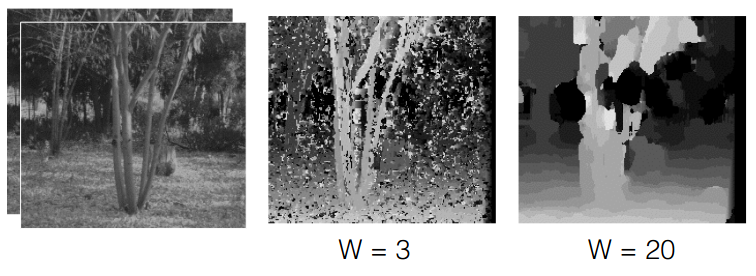
\includegraphics[width=0.85\textwidth]{pictures/03_windowsize.png}
  \caption[Effekt der Fenstergö{\ss}e bei Disparitätenkarten]{Effekt der Fenstergrö{\ss}e, (Kris Kitani - Carnegie Mellon University, 2020)}
\end{figure}

Die Fenstergrö{\ss}e wirkt sich direkt auf die Disparitätenkarte aus. Sie beschreibt die Verschiebung zwischen den beiden Bildern und enthält noch nicht die gesamte Tiefeninformation. Tiefe wird mit Hilfe der Disparität berechnet, wie gezeigt in Gl. \ref{eq:depth}. Für kleine Fenstergrö{\ss}en enthält die Disparitätenkarte mehr Details aber auch mehr Rauschen. Für gro{\ss}e Fenster ist die Karte glatter und hat weniger Details.

Generell beschleunigt Block Matching die Erstellung der Disparitätenkarte da weniger Vergleiche vorgenommen werden müssen. In Regionen ohne Texturen oder bei Bildern in denen sich Muster oft wiederholen kann das Verfahren fehlschlagen. Teile der Karte sind dann Schwarz und ohne Information. 

\section{Deskriptoren}
Für gefundene Merkmale werden Deskriptoren berechnen. Sie sind sozusagen der Fingerabdruck von jedem Merkmal. Mithilfe des Deskriptors sollen Merkmale eindeutig und zuverlässig wiedererkannt werden können. Vor allem auch dann, wenn sich die Abgebildete Szene zwischen zwei Bildern verändert hat. Ein Interest-Operator bleibt als solcher erkennbar, auch wenn die Region gedreht wird. Schwieriger verhält es sich mit der Skalierung. 
\newline

Mit dem Harris-Detektor können bei einer gro{\ss}en Änderung der Skalierung der Interest-Punkt nicht mehr wiedergefunden werden. Die ersten skalierungsinvarianten Detektoren kamen mit SURF (2006) und SIFT (1999). SIFT (Scale-Invariant Feature Transform) liefert sehr gut Resultate in Verbindung mit Lokalisierungsaufgaben. Allerdings braucht der Deskriptor viel Rechenleistung und ist zu langsam für Echtzeitanforderungen. ORB ist eine weit verbreitete, wesentlich weniger Rechenaufwendige Alternative. Für den Systementwurf wurden zu Beginn beide Algorithmen betrachtet. Zusammen mit der Simulationsumgebung verbrauchten die Visuelle Odometrie SOftware mit SURF zu viele Ressourcen. Der Wechsel zu ORB brachte eine wesentliche Entlastung der CPU.
\newline 

Diese Beobachtung lässt sich einfach durch eine Kategorisierung der Berechnungsmethoden der Algorithmen erklären.

SIFT gehört zu der Klasse der \textit{Histogram of Oriented Gradients} (HOG) Deskriptoren währen ORB zu den \textit{Binären} Deskriptoren zählt. Ein Deskriptor hat immer eine Beschreibung für einen interessanten Pixel und seiner unmittelbare Nachbarschaft  sowie eine Distanzfunktion mit der die Ähnlichkeit zwischen zwei Deskriptoren (des gleichen Typs) bestimmt wird.

\subsection{Histogram Deskriptoren}
\begin{figure}[!ht]
  \centering
  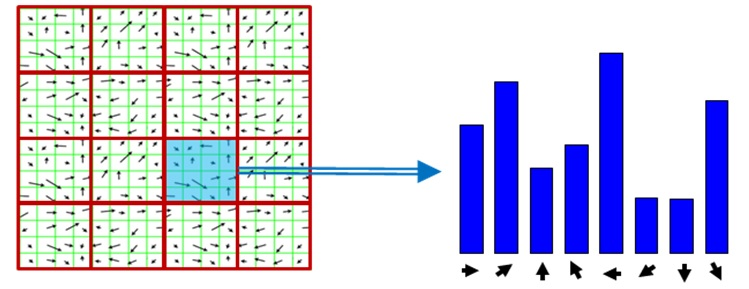
\includegraphics[width=0.75\textwidth]{03_HOG_01.jpg}
  \caption[Histogram Deskriptor aus Gradienten]{Berechnen der Histogramme für die Ausrichtung der Gradienten (Lowe, 1999 \cite{SIFT})}
\end{figure}

Histograms of Oriented Gradients (HOF) Deskriptoren die in der Praxis häufig eingesetzt werden sind SIFT \cite{SIFT} und SURF\cite{SURF}. Im folgenden werden die Rechenschritte für SIFT beispielhaft erläutert.
\newline

Bei dieser Art von Deskriptor wird ein Region um das Merkmal, beispielsweise 16x16 Pixel, genommen. Die Region wird wiederum in kleinere Subregionen unterteilt, beispielsweise 4x4. Für alle Pixel wird die Orientierung berechnet und anschlie{\ss}end der Gradient für die Subregion. Daraufhin kann ein Histogram für die Subregionen erstellt werden.

Durch Aneinanderreihen der Histogramme ergibt sich ein Merkmalsvektor. Für das Beispiel waren es 16 Subregionen mit 8 Histogrammen per Subregion, also ein Merkmalsvektor der mit 128 (16*8) Elementen. 

\subsection{Binäre Deskriptoren}

\begin{figure}[!ht]
  \centering
  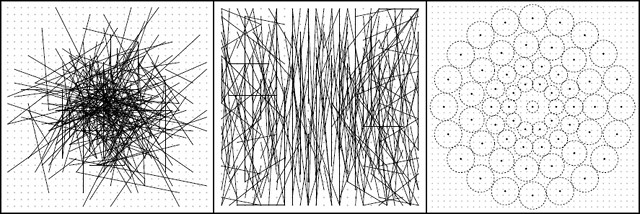
\includegraphics[width=\textwidth]{03_brief_orb_brisk_640.jpg}
  \caption[Muster binärer Deskriptoren]{Deskriptor Muster, von Links nach Rechts: BRIEF, ORB, BRISK. (Heinly, 2012 \cite{binDesc})}
\end{figure}

Anstatt, wie bei HOG Deskriptoren, die Gradienten aller Pixel zu berechnen, werden bei binären Deskriptoren Intensitätswerte verglichen. Das Ergebnis des Vergleichs sind Binärwörter. Diese können direkt durch den XOR-Operator abgeglichen werden, was das Matching deutlich beschleunigt. 

Beispiele für bekannte binäre Deskriptoren sind BRIEF \cite{BRIEF}, ORB \cite{ORB} und BRISK\cite{BRISK}. Binärdeskriptoren können anhand von drei Attributen verglichen werden.

\begin{description}
  \item[Das Abtastmuster] Ein Muster das auf die Region um den Deskriptor gelegt wird. Es werden nur Punkte die auf dem Muster liegen untersucht.
  \item[Ausrichtungskompensation] Eine Methode um die Orientierung des Merkmals zum bestimmen und es zu drehen um Rotation des Merkmals zwischen den Bildern auszugleichen.
  \item[Stichprobenpaare] Auswahl von Punkten die Verglichen wurden welche im Binärwort eingetragen werden sollen. 
\end{description}

Es müssen nicht alle diese Attribute in binären Deskriptor vorhanden sein, sie helfen lediglich bei der Klassifizierung. Wie auch zuvor bei HOG Deskriptoren wird eine Region ausgewählt. Auf die Region wird ein Muster gelegt. Je nach Einstellung werden N Punktpaar auf dem Muster ausgewählt und deren Intensitätswerte verglichen. Ist Punkt A heller als Punkt B ist das Resultat eine 1, sonst 0. Dies wird für die N Punktpaare wiederholt. Anschlie{\ss}end wird ein Strichprobenmenge aus N entnommen und als Binärwort abgelegt. Für das spätere Matching mit einem anderen Deskriptor muss lediglich die Summe über die XOR Verknüpften Binärwörter gebildet werden um die Ähnlichkeit zu bestimmen. Sum(xor(string1, string2)) ist die sog. Abstandsfunktion. Aus der Abstandsfunktion lässt sich schlie{\ss}en, das die Reihenfolge der gespeicherten Werte keine Rolle spielt.


\subsection{ORB - Oriented FAST and Rotated BRIEF}
ORB ist eine Erweiterung des FAST Detektors und BRIEF Deskriptors. BRIEF war 2011 der erste veröffentlichte binäre Deskriptor. Er hat noch kein festes Muster. Stattdessen wird ein zufälliges Muster erstellt. Der Deskriptor erzielt damit eine hohe Wiedererkennungsrate, solange es keine Rotation im Bild gibt, denn es wurde auch noch keine Ausrichtungskompensation implementiert. ORB erweitert BRIEF mit einer entsprechenden Methode und ist damit rotationsinvariant.
Um die Orientierung eines Interest-Operators zu messen verwendet ORB einen \textit{intensity centroid} \cite{Rosin1999MeasuringCP}, bestimmt also den Schwerpunkt der Intensitätswerte. Die Momente der Region errechnen sich zu
\begin{equation}
  \centering
  m_{pq}=\underset{x,y}{\Sigma}x^py^qI(x,y)
\end{equation}
mit I(x,y) als Intensitätsfunktion und p,q als Grad des Moments. Der Schwerpunkt wird berechnet durch
\begin{equation}
  \centering
  C = ( \frac{m_{10}}{m_{00}}, \frac{m_{01}}{m_{00}})
\end{equation}
und schlie{\ss}lich die Richtung durch 
\begin{equation}
  \centering
  \theta = atan2(m_{01}m_{10})
\end{equation}

% !TEX program = xelatex
\chapter{Kamerasysteme}
\label{ch:hardware}
\section{Kamerasensoren}
  \begin{figure}
    \centering
    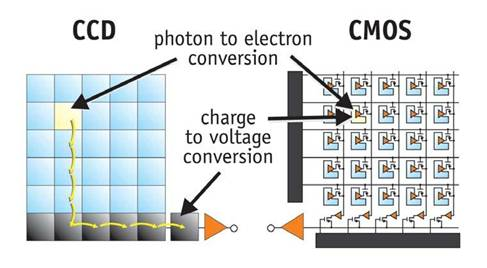
\includegraphics[width=0.75\textwidth]{pictures/04_CCD_CMOS.jpg}
    \caption[Aufbau CCD vs CMOS]{Aufbau CCD vs CMOS (Merolini, 2022 \cite{Merolini.IMG})}
    \label{fig:ccdcmos}
  \end{figure}

  Um eine Schätzung der Pose eines Fahrzeugs in seiner Umgebung vornehmen zu können, muss ein Modell der Umgebung erstellt werden. Kamerasensoren sind externe Sensoren die Eigenschaften und Informationen der Umwelt erfassen.
  \newline  

  Kamerasensoren sind mittlerweile preisgünstig, während die Qualität und Auflösung der Bilder hoch ist. Dadurch sind sie einer breiten Masse von Forschern und Studenten zugänglich, auch ein Grund ist warum visuelle Bildverarbeitungssysteme in der Robotik so verbreitet sind. 
  \newline
  
  Um die Kamerapose durch Visuelle Odometrie zu schätzen muss in jedem Fall ein Weg gefunden werden Informationen über die Distanz zwischen der Kamera und Objekten aus der Umgebung zu gewinnen. Die Tiefe kann mit einer einzelnen Kamera rein algorithmisch geschätzt werden. Mit zwei Kameras lässt sich durch Stereoskopie ein Sonderfall der Epipolargeometrie ausnutzen und Punkte können effizient trianguliert werden. Spezielle Tiefenbildkameras mit Infrarot (IR) Projektion oder Time-of-Flight (ToF) Messungen lösen das Problem vollständig in Hardware. Im folgenden soll auf die wichtigsten Sensoren kurz eingegangen werden.


  \subsection{RGB Kamera mit CCD- oder CMOS-Sensoren}

  \subsubsection{CCD Sensoren}
  Die CCD Technologie wurde Mitte der 70er Jahre erfunden. CCD war damals der Durchbruch der Halbleitersensoren. Die Abkürzung CCD steht dabei für "Charge-Coupled Device".
  \newline
  
  Aufgrund der Funktionsweise des Ladungsträgertransportes werden sie oft mit Eimerketten verglichen. Eine Elektronenschicht liegt auf einer Fotozellen Silizium-Trägerschicht. Auf die Fotozelle einfallendes Licht löst negativ geladene Elektronen aus den Silizium Atomen. Je intensiver das Licht, desto mehr Elektronen lösen sich. Jede Fotozelle ist mit einem Gate verbunden. An das Gate wird eine Spannung angelegt, wodurch die Ladung angezogen werden. Durch gezieltes heben und senken des Potentials werden die Ladungsträger durch die Speicherbereiche geschoben. Die Ladung wandert solange durch das Array, bis der Rand des Sensors erreicht ist. Dort wird das Ladungspaket von einem externen Verstärker in eine Spannung konvertiert.


  CCD ist zeichnet sich durch eine hohe Bildqualität aus. Die Frequenz, mit der der Ladungsträgertransport durchgeführt werden kann, ist jedoch begrenzt und niedriger als bei CMOS. Bei zu hohen Frequenzen würde im CCD zu viel Ladung verloren gehen.
  Das Verschieben der Ladungsträger in CCD Sensoren kann au{\ss}erdem zum sog. Blooming Effekt führen, der bei CMOS Sensoren nicht auftritt.

  \subsubsection{CMOS Sensoren}

  Complementary Metal-Oxide Semiconductor, kurz CMOS, Sensoren sind ebenfalls bereits seid en 1970er Jahren auf dem Markt. Es dauerte jedoch noch einige Jahrzehnte bis die CMOS Technologie die heutige Bildqualität erreichte. Da CMOS-Sensoren neben der hohe Bildraten mittlerweile auch eine gute Bildqualität vorweisen, verdrängen sie CCD-Sensoren aus den meisten Anwendungen. 
  \newline

  Während CCD die Ladungspakete extern in Spannung konvertiert, wird die Ladung bei CMOS bereits im Pixel umgewandelt. CMOS Sensoren die selbst Ladung konvertieren werden deshalb auch als Aktiver Pixel Sensor (APS) bezeichnet.

\begin{figure}[h!]
  \centering
  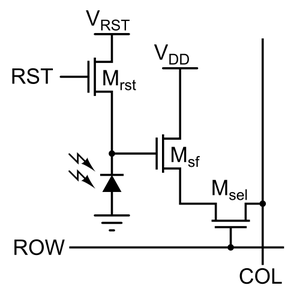
\includegraphics[width=0.4\textwidth]{04_CMOS_3T_circuit.png}
  \caption[3 Transistor CMOS Schaltung]{Schaltung eines einfachen 3 Transistor aktiven Pixels (Wikimedia Creative Commons \cite{Wikimedia})}
  \label{fig:cmos}
\end{figure}

  Ein Einfaches CMOS-Sensor Pixel besteht aus drei MOSFETs und einer Photodiode wie in \ref{fig:cmos} gezeigt. $M_{sf}$ agiert als Verstärker, $M_{rst}$ als Reset der Photodiode und mit $M_{sel}$ kann die Reihe ausgewählt werden.
  \newline

  Wird der Reset geöffnet, erzeugt die Photodiode je nach einfallender Lichtintensität Spannung am Verstärker. Die Spannung wird über den SEL Transistor ausgelesen. 
  \newline

  Wird ein Bild von einem Objekt aufgenommen, das sich in Bewegung befindet, kann es zum sog. Rolling-Shutter Effekt kommen. Durch eine minimale zeitliche Verzögerung bei der Belichtung der Reihen tritt eine Verzerrung im Bild auf. Der Effekt wird Behoben indem zwei weitere Transistoren und ein Kondensator in die Pixelzelle hinzugefügt werden. Dadurch können alle Photodioden zur selben Zeit zurückgesetzt werden und die Belichtungszeit wird synchronisiert.
    

\subsection{Tiefenbildkameras auf Basis von Projektionen}

Das Bekannteste Beispiel dieses Kameratyps ist wohl die ursprünglich für die XBox Spielekonsole eingeführt Kinect 1 Kamera. Ein IR-Transmitter sendet ein bekanntes Muster aus, das von einem Receiver wieder empfangen wird. Objekte auf die das Muster trifft reflektieren das Muster. Je nach Beschaffenheit und Entfernung des Objekts ist das Empfangende Muster Verzerrt und anders skaliert. 
\newline

Das Erfassen von Entfernung durch Musterprojektionen ist sehr empfindlich gegenüber Fremdlicht und hat nur eine begrenzte Genauigkeit. Es gibt daher auch den Ansatz Projektion mit Stereoskopie zu kombinieren wie beispielsweise bei Intels D400 Serie. Neben einer höheren Reichweite ist die Motivation für die IR Projektion hier vor allem ein Nachteil der Stereokamera auszugleichen. Finden sich keine markanten Strukturen im Bild, beispielsweise bei einer wei{\ss}en Wand, kann Stereoskopie versagen. Für solche Fälle führt eine Fusion aus Stereoskopie und Projektion, zumindest Indoor (Reichweite 4m), zu wesentlich Robusteren Ergebnissen. \cite{realsense}

\subsection{Tiefenbildkameras auf Basis von Stereoskopie}

Bei Stereokameras sind zwei Kameras exakt parallel zueinander Ausgerichtet und um eine Baseline b verschoben. Aus der Epipolargeometrie folgt, dass in diesem Fall die Epipole im unendlichen liegen. D.h. die Epipolarlinien verlaufen auf gleicher Höhe durch die Bildebenen der beiden Kameras. Das bedeutet, der Suchraum eines Punktes aus dem linken Kamerabild ist im Rechten Kamerabild enorm beschränkt. Wurde die Abbildung des Punktes in beiden Bildebenen gefunden kann direkt trianguliert werden, da die Baseline bereits bekannt ist. Auf diese weise wird ein Tiefenprofil erstellt. Stereokameras nutzen Kamerasensoren und haben eine entsprechend gro{\ss}e Reichweite. 

\subsection{Time-of-Flight Tiefenbild}

Time-of-Flight Kameras verwenden Photonic Mixing Device (PMD) Sensoren um über ein Laufzeitverfahren die Distanz zwischen Objekten und Kamera zu messen. Zur Laufzeitmessung wird ein gepulster Infrarot Laserstrahl ausgesendet und von einem Receiver empfangen. Dabei wird durch die Phasenverschiebung des Pulses gemessen wie viel Zeit zwischen Senden und Empfangen vergangen ist. Da die Laufzeit von Licht bekannt ist, kann so auf die zurückgelegt Distanz des Laserpulses geschlossen werden.
\begin{equation}
  \centering
  t_D = 2 \cdot \frac{D}{c}
\end{equation}

Mit $t_D$ Zeit, $D$ Distanz und $c$ Lichtgeschwindigkeit $\approx 300\, 000\: \frac{km}{s}$.
\newline

\section{Kamerakonfigurationen}
Da die Visuelle Odometrie auf Kameradaten basiert stellt sich auch die Frage, wie viele Kameras benötigt werden. Grundsätzlich können eine, zwei oder mehrere Kameras beliebig am Fahrzeug montiert werden. Aber nicht jeder Aufbau ist effizient oder sinnvoll.
\newline

Durchgesetzt hat sich monokulare Visuelle Odometrie mit einer Kamera und stereo VO mit zwei Kameras. In dem Versuch die Robustheit von Visueller Odometrie zu erhöhen, vor allem in schlecht belichteten Umgebungen wurden auch Mehrkamerasysteme mit mehr als zwei Kameras untersucht. Liu et al. untersuchten 2019 ein Multi-Stereokamera Setup \cite{mulVO_2019} und erzielten bessere Ergebnisse für Nachtfahrten mit einem Offline-Dataset. Mhiri et al. veröffentlichten bereits 2014 eine Methode in der sie Visuelle Odometrie mit klassischer SfM und Machine Learning kombinierten um die Odometrie aus einem Mehrkamerasystem mit zu schätzen, bei dem die Kameras nicht synchronisiert wurden \cite{Mhiri_2014}.

Mehrkamerasysteme sind eine Seltenheit um sehr spezielle Problemstellungen zu lösen. Weitaus häufiger wird Visuelle Odometrie durch Sensorfusion mit anderen Sensoren kombiniert um dei Robustheit zu erhöhen. Es sit au{\ss}erdem zu beobachten, dass der Trend in die entgegengesetzte Richtung geht. Viele, in den letzten Jahren veröffentlichte Paper, untersuchen monokulare Visuelle Odometrie. Monokulare Visuelle Odometrie ist bereits so lange bekannt wie Stereo Visuelle Odometrie, mittlerweile ist die Technik jedoch weit genug fortgeschritten um monokulare Systeme mit Neuronale Netze (lernende Visuelle Odometrie Verfahren) zu implementieren, welche die Nachteile von monokularen Systemen beheben sollen.   

\subsection{Monokulare Kamerasysteme}
Bei monokularen Kamerasystemen wird die Odometrie anhand aufeinanderfolgender Bilder einer einzelnen Kamera geschätzt. Der Vorteil dabei ist, das weniger Hardware benötigt wird. Das grö{\ss}te Problem ist die Tiefenschätzung. Ohne eine bekannte Basislinie, wie bei Stereokameras, muss die Skalierung zwischen den Bildern ebenfalls geschätzt werden. Dadurch erhöht sich die Drift des Systems. Monokulare und Stereo Visuelle Odometrie haben sich über die Zeit als zwei unterschiedliche Forschungsgebiete entwickelt. Dennoch kann monokulare Visuelle Odometrie auch für stereo Visuelle Odometrie interessant werden, wenn der Abstand zu Szene wesentlich grö{\ss}er als die Basislinie ist. In dem Fall wird aus der stereo eine mono Visuelle Odometrie. Für autonome Fahrzeuge trifft dieser Fall i.d.R. nicht ein.   


\subsection{Stereo Kamerasysteme}
Stereokameras setzen sich aus zwei Kameras zusammen, die exakt parallel ausgerichtet sind und eine feste Basislinie haben. Der Grund dafür sind die besonderen Eigenschaften der Epipolargeometrie solch eines Aufbaus. Dadurch können Pixel schnell Trianguliert werden und so eine Tiefenkarte aus der Geometrie geschätzt werden. Stereokameras sind günstig, liefern qualitativ hochwertige Bilder und sind seid Markteinführung der Kinect Kamera auch bei Robotik Enthusiasten verbreitet. 
\begin{figure}[!ht]
  \centering
  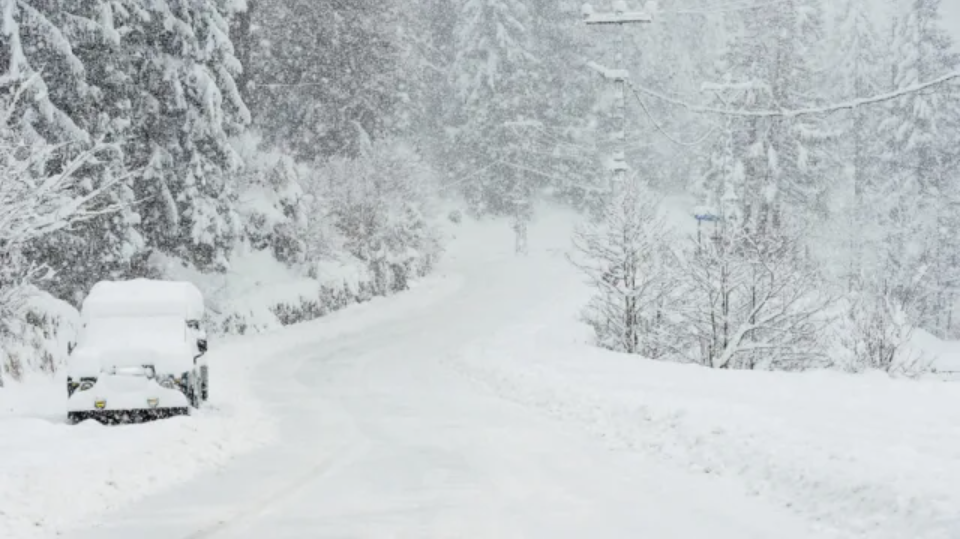
\includegraphics[width=0.75\textwidth]{04_snow.png}
  \caption[Verschneite Stra{\ss}e]{Szenen mit wenig Textur sind auch bei ausreichender Beleuchtung eine Herausforderung für Stereokamera Triangulation (Shutterstock ID 1248440977, 2022)}
\end{figure}
Auch wenn die Triangulation ein schnelles und Zuverlässiges Verfahren ist, muss die abgebildete Szene bestimmte Voraussetzungen Erfüllen. Ohne ausreichende Beleuchtung oder Textur arme Umgebungen führen dazu, dass Pixel nicht abgeglichen werden könne. Ohne ein erfolgreiches Matching kann die Triangulation nicht stattfinden.  


\subsection{RGB mit Tiefenbildkamera}
Für ein Kamerasystem mit RGB-D Kamera wird der gleiche Odometrie Algorithmus implementiert wie für Stereokameras. Software seitig gibt es lediglich den Unterschied, dass das Stereo-Matching und die Triangulation entfällt. Falls diese Schritte nicht ohnehin bereits im Kamerasystem abgearbeitet wurden.

Theoretisch kann eine RGB-D Kamera dort Datenpunkte liefern, wo eine reguläre Stereokamera versagt. Schlechte Lichtverhältnisse und wenig Struktur im Bild haben keine negativen Auswirkungen. Genauso wie sich wiederholende Muster und Asphalt kein Problem darstellen. Dafür wird RGB-D aufgrund des Infrarotlasers durch Sonneneinstrahlung und Reflexionen von Spiegelnden Oberflächen gestört. Dazu kommt, dass die meisten RGB-D Kameras nur über eine geringe Reichweite von wenigen Metern verfügen. In der Praxis werden sie daher überwiegend in geschlossenen Räumen verwendet. In den letzten Jahren kamen jedoch bereits ein paar Kameras auf den Markt, die speziell für den SLAM Einsatz entwickelt wurden und grö{\ss}ere Reichweiten versprechen \cite{rgbd}.

\subsection{Rektifizierung}
\begin{figure}[!ht]
  \centering
  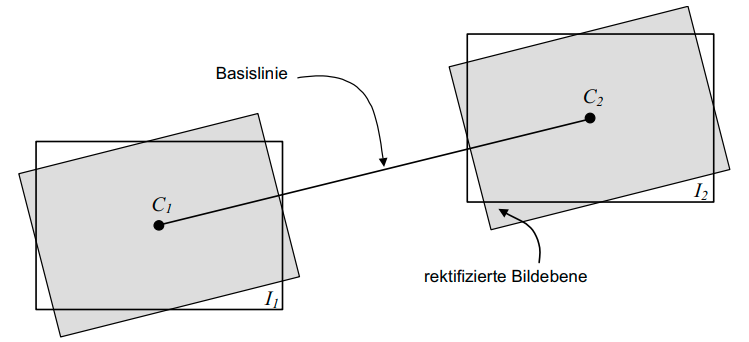
\includegraphics[width=.75\textwidth]{04_rekti2.png}
  \caption[Rektifikation der Stereobildebenen]{Bildebenen einer Stereokamera werden Rektifiziert. Dadurch verlaufen die Epipolarlinien parallel zu den Bildzeilen. (Scheer, 2005 \cite{stereoSchreer})}
\end{figure}
   
Das simulierte Stereokamerasystem das in CARLA am Fahrzeug angebracht wird ist ideal. Alle Kameraparameter sind aus der Konfiguration bekannt. Zwischen der linken und rechten Kamera gibt es keine ungewollte Verschiebung. In realen Systeme sind Stereokameraufbauten i.d.R. nur näherungsweise parallel.

Deshalb werden die Bilder durch eine softwareseitige Drehung in ein tatsächlich achsenparalleles System transformiert. Dieses virtuelle Drehen wird als Rektifizierung bezeichnet und die Kamerabilder als rektifiziert. Die Transformation ist linear und bei erfolgreich transformierten Stereobilder liegen die Epipole im unendlichen. 

Für eine Rektifikation müssen die internen Kameraparameter bekannt sein. Diese sog. intrinsischen Parameter liefert entweder der Kamerahersteller oder werden durch Kamerakalibrierung ermittelt. Wichtig ist zudem, dass sich die Kamerazentren $(C_1 , C_2)$ durch die Rektifizierung nicht verschieben. 
\chapter{Systementwurf}
%Bildgewinnung
\section{Erzeugen von Sensoroutput}
%
\subsection{Kameradaten}
\begin{figure}[h!]
  \begin{center}
    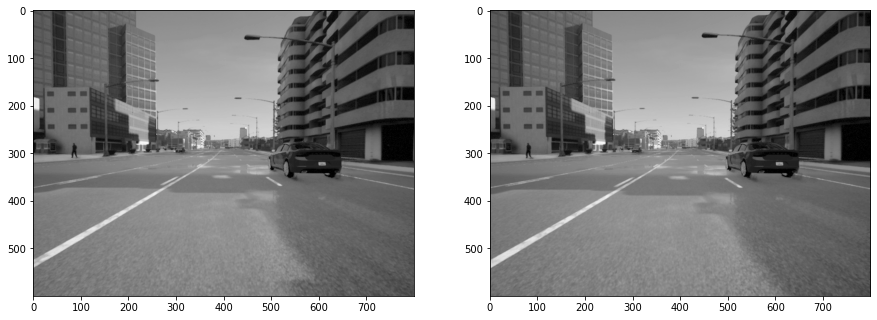
\includegraphics[width=\textwidth]{pictures/load_images_systementwurf.png}
    \caption[Eingansdaten Bilder aus Stereoaufbau in CARLA Simulator]{Grayscale konvertierte RGB Bilder aus Stereo Setup auf Fahrzeug in CARLA Simulator montiert.}
  \end{center}
\end{figure}
%
Alle Sensoroutputs werden im Simulator generiert. 

Zu Beginn kommen Kameradaten in das System. Entweder in Form von zwei RGB Bildern, die um eine Baseline $b=50 cm$ verschoben aufgenommen wurden. 
%
Oder als RGB und Depth Image Paar.

\subsection{Node für Kamerasynchronisation}
\begin{center}
  \begin{figure}[h!]
    \centering
    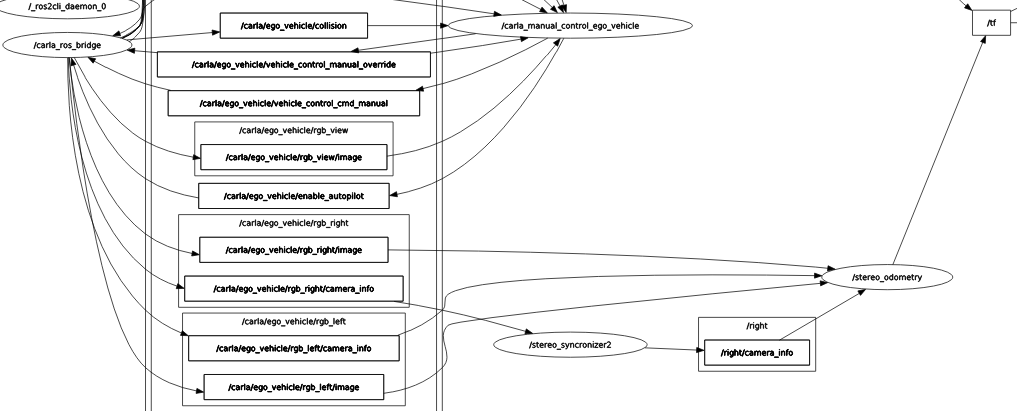
\includegraphics[width=\textwidth]{pictures/06_ros_topic_graph.png}
    \caption[Graph der ROS2 Topics]{Graph zeigt im unteren Teil die Verknüpfungen der Topics aus der Simulator-Bridge bis zur gesucht Transformation.}
    \label{fig:rosgraph}
  \end{figure}
\end{center}

Für die Visuelle Odometrie wird ausschlie{\ss}lich der RGB Kamerasensor und der Pseudosensor Depth Map verwendet. Für die Auswertung werden zusätzlich die Ground Truth Daten des Pseudosensors aufgenommen. Die Bridge konvertiert die Sensordaten aus der Simulation in den sensor\_msg Datentyp und veröffentlicht die Nachrichten auf ein entsprechendes Topic im Netzwerk.
\newline

Eine CameraInfo.msg Nachricht enthält:

\subsubsection*{Die 3x3 Kamera-Matrix $K$}
$K$ enthält die intrinsischen Parametern des Rohbildes (enthält ggf. Verzerrungen). $K$ projiziert 3D Punkte der Kamera-Koordinaten-Ebene auf 2D Pixel-Koordinaten mit $f_{x/y}$ Brennweite und Bildmittelpunkt $c_{x/y}$

\begin{displaymath}
K = 
\begin{pmatrix}
f_{x} & 0 & c_{x}\\
0 & f_{y} & c_{y}\\
0 & 0 & 1
\end{pmatrix}
\end{displaymath}

\subsubsection*{Die 3x3 Rektifizierungsmatrix $R$}
$R$ ist eine 3x3 Rotationsmatrix, die das Kamera Koordinatensystem an der idealen Bildebene ausrichtet, damit die Epipolarlinien beider Bilder parallel sind.

\subsubsection*{Die 3x4 Projektionsmatrix $P$}
Die Projektionsmatrix enthält die intrinsischen Parameter nach der Rektifizierung. Mögliche Verzerrungen wurden durch einen Kamera-Kalibrierungsschritt korrigiert. Unter Verwendung der Simulierten CARLA Sensoren existiert keine Verzerrung und die Parameter gleichen der Kameramatrix K.
\begin{displaymath}
P = 
\begin{pmatrix}
f_{x}' & 0 & c_{x}' & T_{x}\\
0 & f_{y}' & c_{y}' & T_{y}\\
0 & 0 & 1 & 0
\end{pmatrix}
\end{displaymath}
Für Stereokameras entspricht der vierte Zeilenvektor $\left(\begin{smallmatrix}Tx & Ty & 0\end{smallmatrix}\right)'$ der Position des optischen Zentrums der zweiten Kamera im Frame der ersten. Die erste Kamera ist dem zu folge immer $Tx = Ty = 0$. Ohne Korrekturschritt wäre das auch für die zweite Kamera der Fall. Stattdessen berechnen sich die Parameter für die zweite Kamera zu:
\begin{align*}
T_{y}=& 0\\
T_{x}=&-f_{x} * B
\end{align*}
Für ein horizontal ausgerichtetes Setup, mit B für die Baseline zwischen den Kameras.
\newline 


CARLA bietet keinen Stereokamera Sensortyp an. Es müssen zwei einzelne Kamerasensoren mit der korrekten Ausrichtung am Fahrzeug initialisiert werden. Über die Bridge werden die Kameras allerdings auch als voneinander unabhängige Kameras veröffentlicht. 

Anstatt einen neuen Sensortyp in CARLA zu implementieren wurde ein ROS2 Node zum ändern der Nachricht geschrieben. Der Node abonniert das Topic der rechten Kamera. Die Information zu den Kameraparametern werden entsprechend der Stereokamera angepasst und als neue CameraInfo.msg veröffentlicht. Andere Nodes können jetzt einfach das geänderte Kamera Topic abonnieren anstelle des Topics von der Bridge.

%%%%
%
\section{Stereo Visuelle Odometrie Ablauf}
%
\begin{figure}[!h]
  \begin{center}
    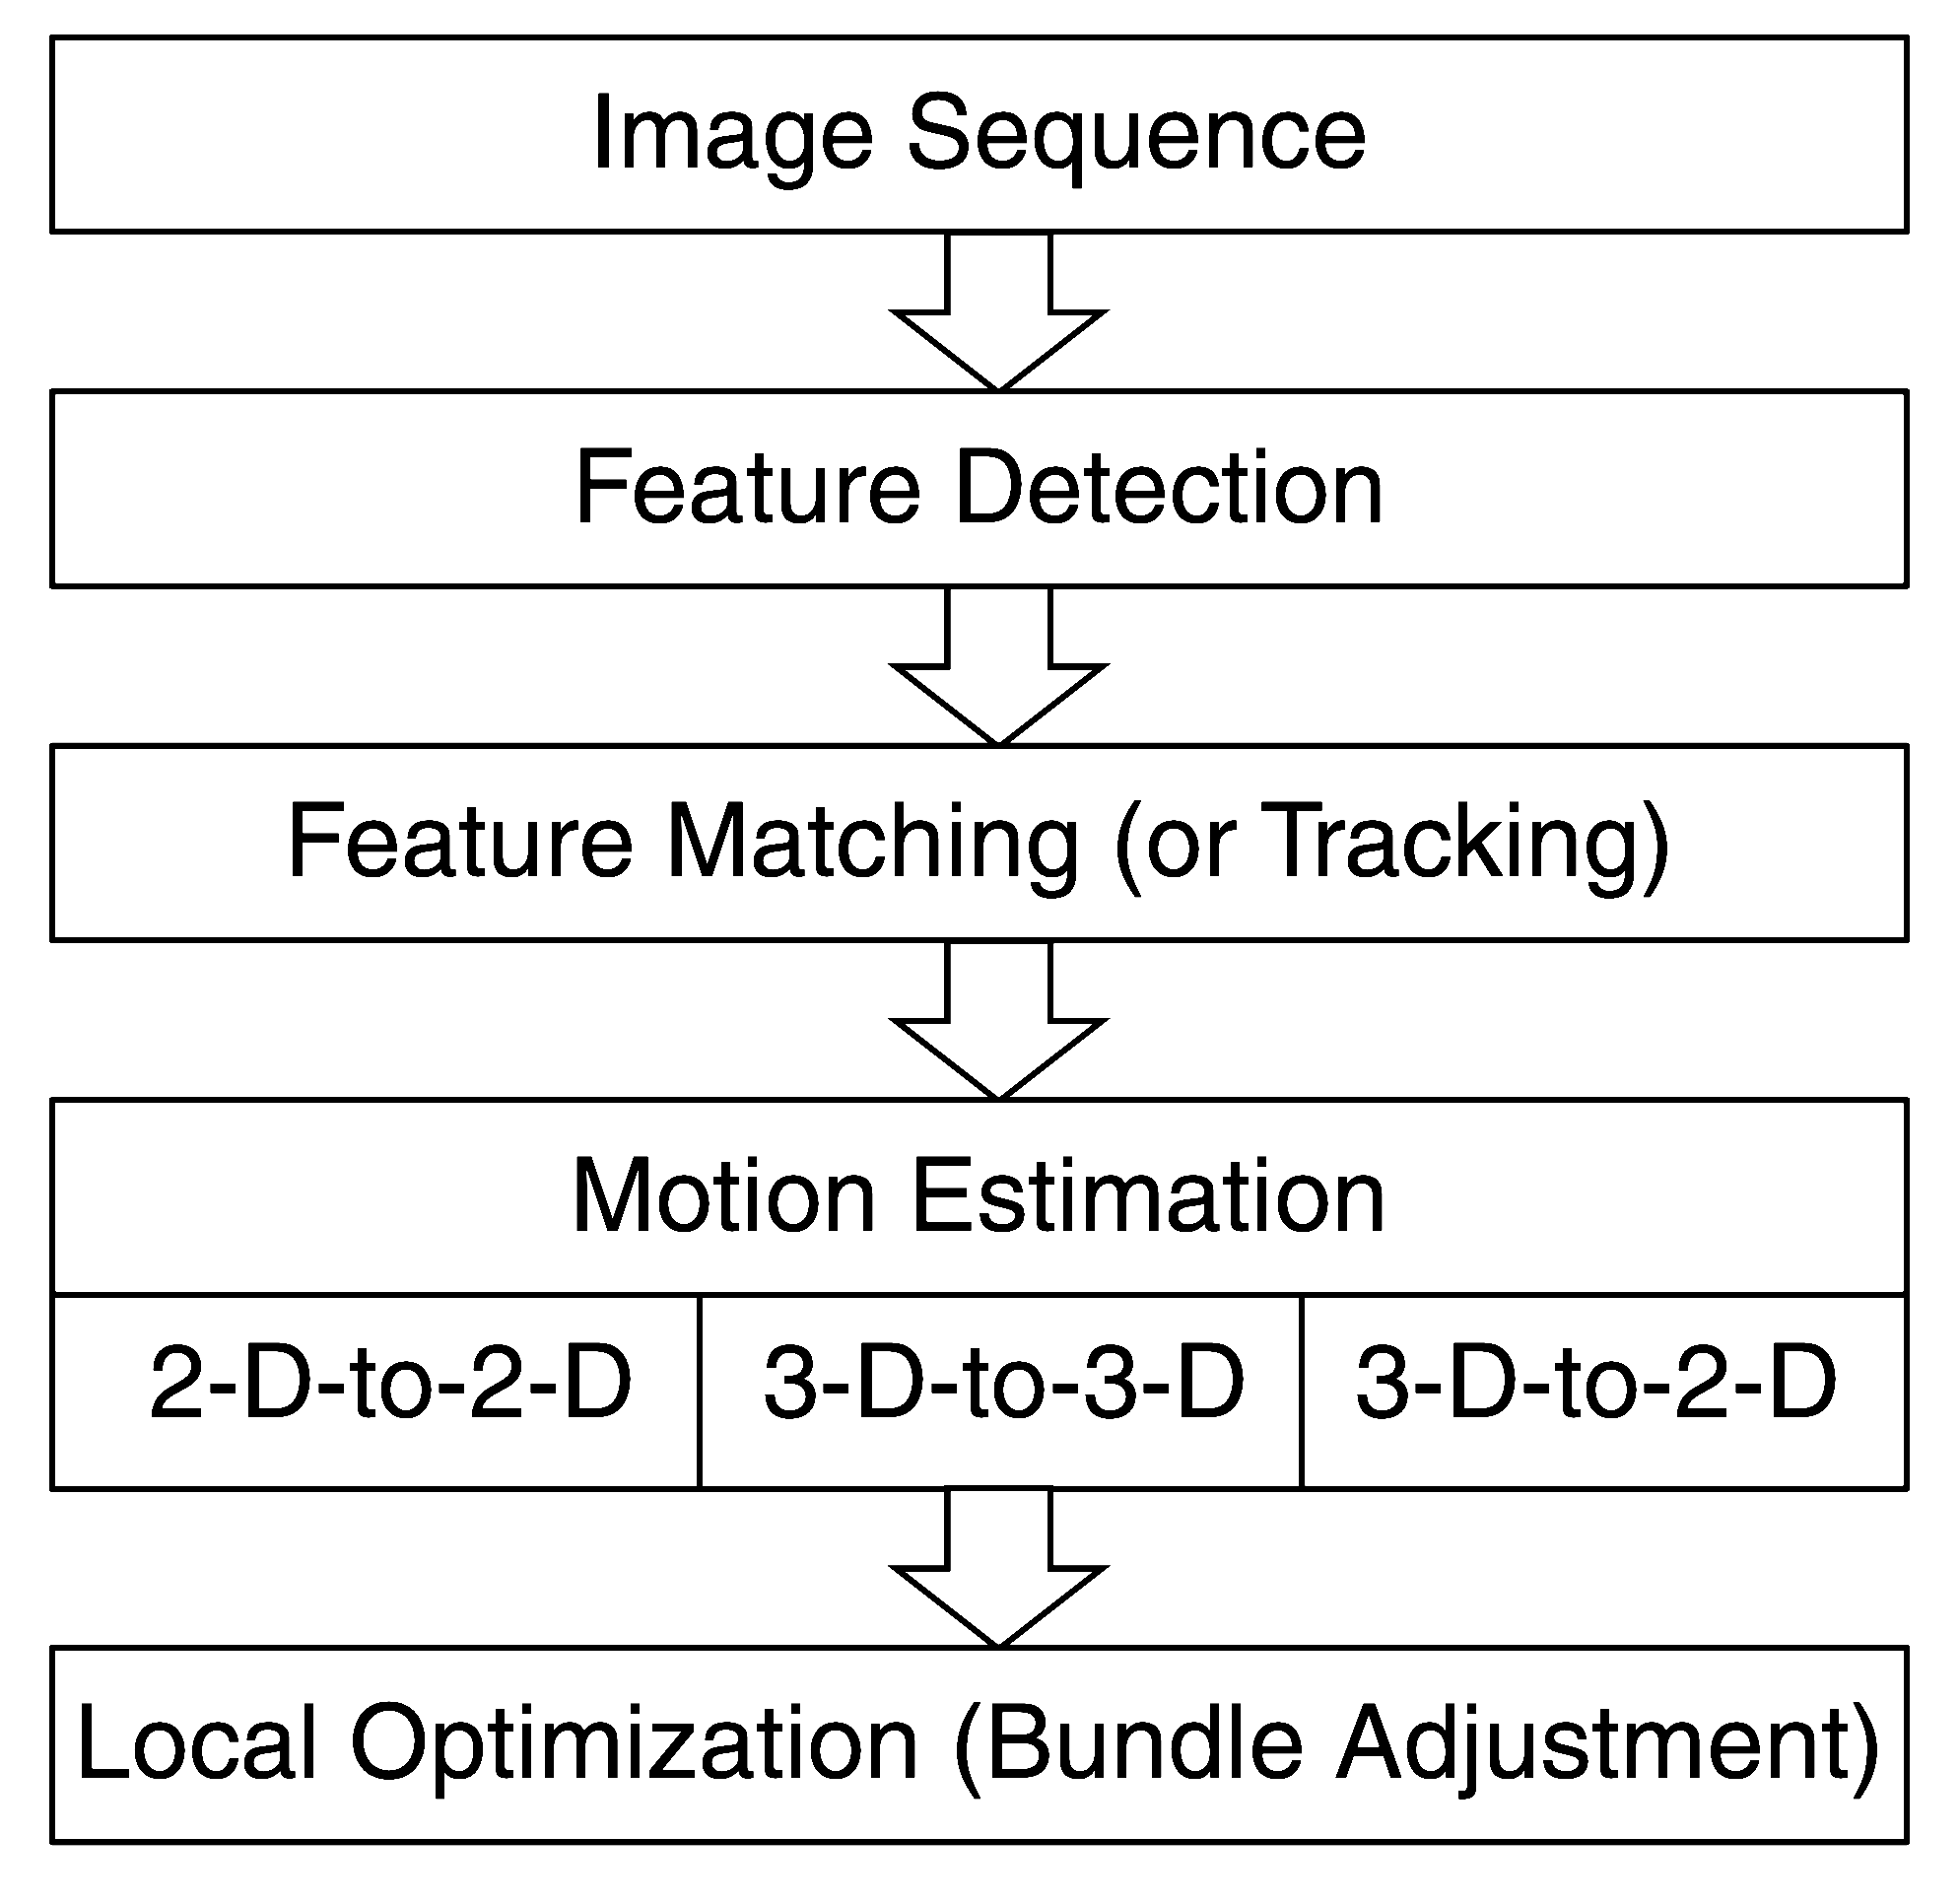
\includegraphics[width=0.45\textwidth]{pictures/vo_pipeline_systementwurf.png}
  \end{center}
  \caption[Visuelle Odometrie Pipeline]{Klassische Pipeline die bei der visuellen Odometrie durchlaufen wird. (In Anlehnung an Scaramuzza, 2011 \cite{ScFrVO})}
\end{figure}
%
%Pipeline
Die Visuelle Odometrie ist ein Verfahren, bei dem die Trajektorie inkrementell geschätzt wird. Der Algorithmus bzw die sog. Visual Odometrie Pipeline wird für jede Schätzung durchlaufen.

\subsection{Merkmalsdetektion}

\begin{figure}[h]
  \begin{center}
    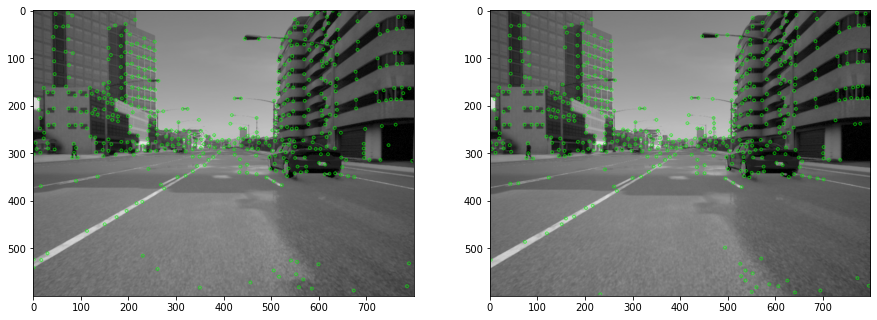
\includegraphics[width=\textwidth]{pictures/feature_detection_systementwurf.png}
    \caption[Merkmalsdetektion in einer CARLA Szene]{Merkmalsdetektion in zwei aufeinanderfolgenden Bildern einer CARLA Szene}
  \end{center}
\end{figure}

Es werden zwei aufeinanderfolgende Bilder $Img_{t-1}$ und $Img_{t+0}$ auf Merkmale untersucht. Die Bilder stammen aus der linken Kamera bei Stereo RGB Setup bzw aus der RGB Kamera beim RGB-D Setup.
\newline

Die Suche nach Merkmalen erfolgt über einen Detektor. Untersucht werden ORB und GFTT. GFTT (Good Features To Track) ist die Implementierung des Shi-Tomasi Interest-Operators und detektiert Kanten im Bild. GFTT ist ein reiner Detektor.

Alternativ wird die Extraktion mittels ORB Detektor betrachtet. Für diesen Fall werden die Merkmale durch einen oriented FAST-9 Detektor gesucht. In anderen Arbeiten wurde gezeigt, dass der ORB Detektor 64 mal schneller Merkmale extrahiert als GFTT, bei gro{\ss}en Veränderungen der Skalierung oder des Kamerawinkels allerdings weniger Merkmale liefert.\cite{Mouats.PerfD}
\newline

Die Detektoren liefern Keypoints für die gefundenen Merkmale. Diese werden an Detektor-Algorithmen übergeben. Ein Detektor ist vergleichbar mit einem Fingerabdruck die eindeutige Beschreibung eines Merkmals. Ein durch einen Detektor beschriebener Keypoint lässt sich auch nach Veränderung im Bild wiederfinden. Diese Robustheit gegenüber Veränderungen wird als Invarianz bezeichnet und ist eine wesentliche Voraussetzung für das MAtching von Merkmalen zwischen zwei Zeitschritten.

Als Deskriptor wird in jedem Fall ORB verwendet.
%
\subsection{Matching von Merkmalen}
% Frame 2 Frame
Beim Matching von Merkmalen wird bestimmt welche Deskriptoren in beiden Bildern auftreten. Durch die Bewegung der Kamera können Merkmale aus der Szene das Bildfeld verlassen bzw hinzugekommen sein. Au{\ss}erdem können Merkmale zB verdeckt  worden sein.\\
Matches sind eine Menge von Deskriptoren, die für beide Bilder $Img_{t-1}$ und $Img_{t+0}$ gültig ist. Durch diese Menge wurde eine Beziehung zwischen den Bildern hergestellt.


Der simpelste Algorithmus für das Matching ist die Implementierung von Brute Force. Als erfolgreiches Match gilt ein Vergleich innerhalb einer Suchregion mit der kleinsten Distanz. Brute Force Matcher liefern gute Ergebnisse, vergleichen allerdings sehr viele Merkmale. Daher ist Brute Force die langsamste Methode für den Abgleich.
\newline

Eine Methode die für gro{\ss}e Mengen an Deskriptoren (>1000) \cite{Mouats.PerfD} schneller sein kann ist der FLANN (Fast Library for Approximate Nearest Neighbors) basierte Matcher. FLANN baut einen KD-Baum und gleicht Deskriptoren nur in einer Nachbarschaft ab. Dadurch werden gute Matches schnell gefunden, das Resultat sind aber nicht zwangsläufig das best-möglichste. Eine Erhöhung der Qualität der Ergebnisse kann über Parameter erfolgen, führt aber zu höheren Kosten in der Laufzeit und erhöht die Gesamtausführungszeit.\\
%
\begin{figure}[!h]
  \begin{center}
    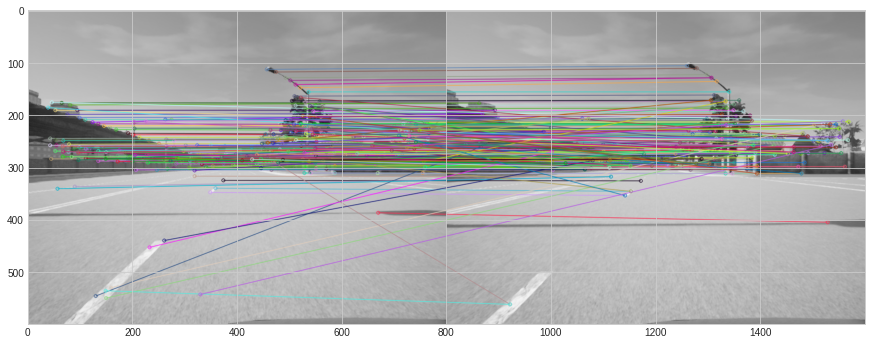
\includegraphics[width=\textwidth]{pictures/bf_matching_no_crosscheck_systementwurf.png}
    \caption[Brute Force Matching ohne Crosscheck]{Brute Force Merkmalsabgleich ohne Cross Checking in zwei aufeinanderfolgenden Bildern einer CARLA Szene.}
  \end{center}
\end{figure}
%
Um ein möglichst robustes Ergebnis zu erzielen wird der Brute Force Matcher mit Cross-Check verwendet. Beim Cross-Check werden die Resultate der beiden Bilder darauf Verglichen, ob das beste Match in Set A auch das beste Match in Set B war und umgekehrt. 
Cross-Checking liefert konsistente Resultate und ist eine Alternative zum sonst verwendeten Lowes Ratio Test für das Filtern von Ausrei{\ss}ern. \cite{cvdocMatch}
%
\begin{figure}[!h]
  \begin{center}
    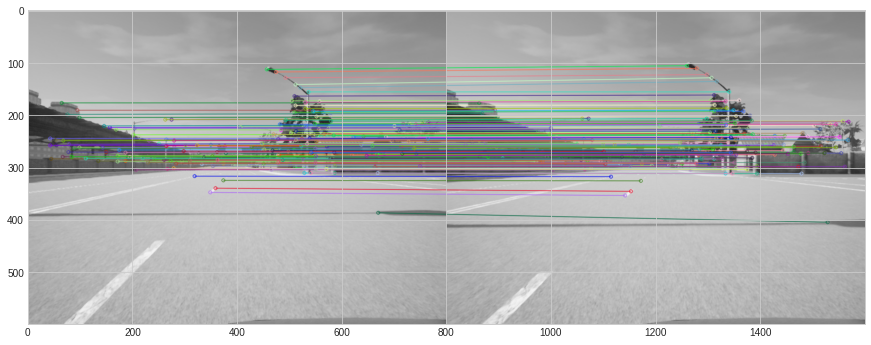
\includegraphics[width=\textwidth]{pictures/bf_matching_with_crosscheck_systementwurf.png}
    \caption[Brute Force Matching mit Crosscheck]{Brute Force Merkmalsabgleich mit Cross Checking in zwei aufeinanderfolgenden Bildern einer CARLA Szene.}
  \end{center}
\end{figure}
%
In der OpenCV Implementierung des Brute Force Matcher kann au{\ss}erdem ebenfalls ein Nachbarschafts-beschränkung mitgegeben werden. Für Binäre Deskriptoren wie ORB wird hier am besten die Hamming Distanz anstatt des Standardmä{\ss}igen Euklidischen Abstands gewählt.


\subsection{Tiefeninformation}
Die zwei simulierten Setups beziehen ihre Tiefeninformation aus unterschiedliche Weise. In jedem Fall kann auf Pixelebene die Tiefe als ein zusätzlicher Kanal betrachtet werden.
%
\begin{figure}[!ht]
  \begin{center}
    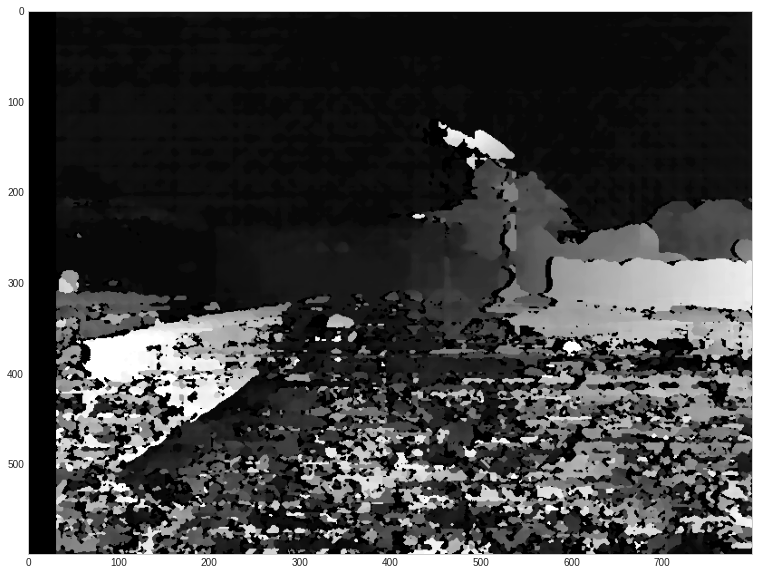
\includegraphics[width=0.5\textwidth]{pictures/disparity_notebook.png}
    \caption[Disparitätenkarte]{Disparitätenkarte als Ergebnis eines Stereo Matchings einer CARLA Szene.}
  \end{center}
\end{figure}
%
Beim Stereo RGB Kamera Setup liegen die Tiefeninformationen nicht direkt vor sondern werden über Triangulation von Stereomatches unter Zuhilfenahme der Epipolargeometrie berechnet.  Daraus entsteht die sog. Disparitätenkarte. Bei der Programmierung wird hier ein StereoMatcher verwendet. StereoMatcher sind Matching Algorithmen die die Epipolaren Beschränkungen gezielt zur Beschleunigung der Suche einsetzen. Im vorgestellten Systementwurf wird ein in OpenCV implementierter Semi-Global Matching Algorithmus basierend auf einem 2008 von Hirschmüller veröffentlichten Paper verwendet. \cite{Hirsch.SGBM}
%

RGB-D liefert das Tiefenbild direkt, weshalb keine zweite Kamera und keine Berechnung der Verschiebung zwischen den Bildern nötig ist. Real wird die Tiefe über eine Time-of-Light Messung bestimmt. In der Simulation werden die Tiefenbilder direkt vom Simulator ausgegeben mit einer maximalen Tiefe von einem Kilometer, was reale ToF Kameras bei weitem übertrifft.

\subsection{Bewegungsschätzung}

Die Bewegungsschätzung erfolgt von Frame zu Frame (F2F). Für jedes Match werden die Pixelkoordinaten aus den Keypoints ausgelesen. Dadurch liegen zwei 2D Punktmengen für die beiden Bilder vor. Für die Matches aus dem vorherigen Bild $Img_{t-1}$ werden au{\ss}erdem die Tiefeninformation der Pixel zu den Punkten hinzugefügt. Die Information lässt sich bei Stereo Kamera aus der Disparitätenkarte lesen bzw aus dem Tiefenbild bei einer RGB-D Kamera.

Dadurch liegen schlie{\ss}lich eine 3D Punktmenge der Matches für $Img_{t-1}$ und ine 2D Punktmenge für $Img_{t+0}$ vor.

Die 3D Punkte aus dem vorherigen Zeitschritt dienen als Objekte im Weltkoordinatensystem zu denen die aktuelle Punkte in Bezug gesetzt werden. Es wird die Transformation gefunden für die der Re-Projektionsfehler am geringsten ist. Die Reprojektion die hier betrachtet wird läuft von den 3D Punkten durch die 2D Bildpunkte zum Kamerabrennpunkt. (Anders als beim Bundle Adjustment wo die Reprojektion auf die 2D Bildpunkte betrachtet wird).


Das Problem des Schätzens der Pose aus Korrespondenzen aus 3D Referenzpunkten und ihrem 2D Abbild in einer kalibrierten Kamera wird als Perspective-from-N-Points Problem (PnP) bezeichnet und ist fundamentaler Bestandteil vieler Computer Vision Anwendungen. Erste Lösungen der Problemstellung existieren bereits seid 1841. Heute wird i.d.R. eine Kombination aus PnP mit RANSAC verwendet, da PnP empfindlich gegenüber Ausrei{\ss}ern ist. RANSAC filtert Ausrei{\ss}er.

Mathematisch wird bei PnP Algorithmen versucht eine eindeutige Lösung für ein überbestimmtes Gleichungssystem aus Polinomgleichungen zu bestimmen. Ohne weitere Information zu den Punkten werden mindestens 4 Punkte für eine eindeutige Lösung benötigt. Die Berechnung für P4P ist jedoch wesentlich komplexer als für $p \geq 5$ weshalb wenn möglich, wie bei der Visuellen Odometrie oder allgemein SLAM Verfahren mit mindestens 5 Punkten berechnet wird.
\newline

Unter Zuhilfenahme des Lochkamera-Modells und der Kameramatrix $K$ werden die 3D Punkte aus der Bildebene (Pixelkoordinaten) in das Kamerakoordinatensystem transformiert.
%
\begin{equation}
\label{eq:sshort}
    sP_{c} = K[R | T]p_{w}
\end{equation}
%
\begin{equation}
  s 
  \begin{bmatrix}u\\v\\1\end{bmatrix} = \begin{bmatrix}
  f_x & \gamma & u_0\\
  0 & f_y & v_0\\
  0 & 0 & 1
  \end{bmatrix}\begin{bmatrix}
  r_{11} & r_{12} & r_{13} & t_{1}\\
  r_{21} & r_{22} & r_{23} & t_{2}\\
  r_{31} & r_{32} & r_{33} & t_{3}\\
  \end{bmatrix}
\begin{bmatrix}x\\y\\z\\1\end{bmatrix}
\end{equation}

Umformung zu 

\begin{equation}
  P_c = K^{-1} \cdot (s \cdot [u, v, 1])
\end{equation}

Bei PnP wird also die Bewegung aus einer 3D zu 2D Transformation geschätzt.

\begin{equation}
\label{eq:tmatrix}
  \begin{split}
T_{k} &= 
    \begin{pmatrix}
    R_{k,k-1} & t_{k,-1}\\
    0 & 1
    \end{pmatrix} \\
    \\
    &= \arg\min_{T_{k}} \sum_{i=1} \left\|p_{k}^i - \hat{p}_{k-1}^i \right\|^2,
  \end{split}
\end{equation}
%

%
\subsection{Pose Update und Verlorene Odometrie}
Ausgabe der Schätzung ist ein Translationsvektor $t$ und eine Rotationsmatrix $R$ für die aktuelle Position. Durch Multiplikation der vorherigen Pose mit $R|t$ wird die aktuelle Pose berechnet. Addition der Posen gibt die Trajektorie.

An dieser Stelle wird ein Update der Output Odometrie vorgenommen und die ROS Transformation von $tf\: \/odom\: \rightarrow\: \/base\_link$. Die ausgegebene Kovarianz wird berechnet durch die Median Absolute Deviation (MAD) zwischen den 3D Merkmalskorrespondenzen.

\begin{equation}
  MAD = median (\|X_i - \tilde{X}_i \|)
\end{equation}

Unter Umständen konnte keine Schätzung durchgeführt werden, Beispielsweise weil nicht genügend Matches gefunden werden konnten. In diesem Fall wird die aktuelle Kameraposition auf die letzte gültige Kameraposition gesetzt.
\chapter{Implementierung}
\label{ch:implementierung}

Um das System zu implementieren und zu testen wurde bereits existierende Software und Bibliotheken verwendet die in ihrer Funktion und Anwendung im Projekt kurz erläutert werden sollen.


\section{Simulationsumgebung}
\subsection{Simulator CARLA}
Der gesamte Systeminput wird durch den CARLA Simulator\cite{Dosovitskiy17} erzeugt. Nach eigener Aussage ist die Motivation hinter dem Projekt die Demokratisierung in der Forschung und Entwicklung autonomen Fahrens. CARLA (Car learning to act) ist ein Open-Source Simulator basierend auf der Unreal Engine 4. Die Engine ist kostenlos für nicht-kommerzielle Nutzung und bietet eine Rendering, physikalische Modelle (PhysXVehicles) und NPC Logik für Fu{\ss}gänger und andere Verkehrsteilnehmer. CARLA startet als Server mit einer Python Client API. Über die API können Parameter der Simulation wie z.B. die Map oder das Wetter gesetzt werden. Ein gespawntes Fahrzeug ist ein Client der über Sockets mit dem Server kommuniziert. Die echte Position des Fahrzeugs wird über einen Ground Truth Pseudo-Sensor ausgegeben.


\subsection{ROS2 Framework für Prozesskommunikation}

\begin{figure}[h!]
	\centering
	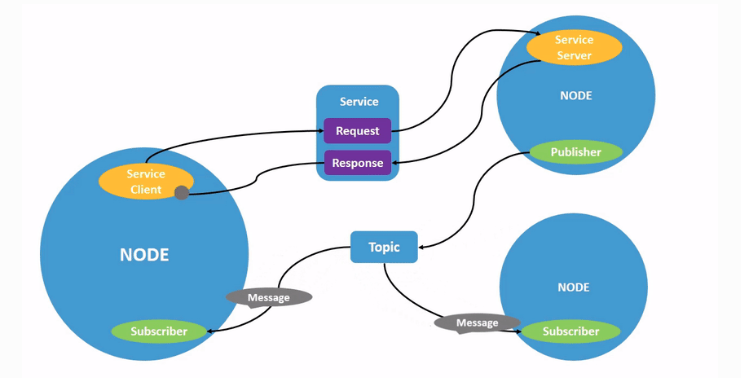
\includegraphics[width=0.8\textwidth]{pictures/06_ROS_nodes.png}
	\caption[ROS2 Node Netzwerk]{Ein ROS2 System besteht aus vielen Nodes die Nachrichten über eine Publish-Subscriber Architektur austauschen. (ROS2 Dokumentation, 2022)}
\end{figure}


Das Robot Operating System ROS2 wird seid 2007 entwickelt und besteht aus einer Sammlung von Bibliotheken und Tools für Robotik Anwendungen. Anders als der Name vermuten lässt, ist ROS2 kein in sich geschlossenes Betriebssystem sondern ein Framework das unter Linux betrieben werden kann. ROS2 und darin zur Verfügung stehenden Software sind Open Source.
\newline

In einem ROS2 System läuft jeder Prozess in einem Node. Ein Programm kann aus mehren Nodes bestehen aber ein Node sollte immer nur einen Zweck erfüllen. Dadurch werden die Systeme Modular und ein Node kann in unterschiedlichen Systemen eingesetzt werden. Bei der Initialisierung eines Nodes können Einstellungen durch sog. Parameter übergeben werden. Jeder Node verwaltet seine eigenen Parameter. Beispielsweise werden für die Stereo und RGB-D Odometrie zwei Nodes vom selben Modul mit unterschiedlicher Parametrierung instanziiert.
\newline

Alle Daten im ROS2 Netzwerk werden in ROS2 Message Datentypen gepackt. Die Nachrichten werden über ein Publish-Subscriber-Architektur im Netzwerk verteilt. Jeder Node kann beliebig viele Topics veröffentlichen oder abonnieren. Das Topic agiert als Datenbus des Systems.\newline 
Der gro{\ss}e Vorteil dieser Architektur ist die Einführung eines Standards für die Schnittstellen der Programme. Ohne Veränderung an dem Node für die Visuelle Odometrie vornehmen zu müssen, kann die Datenquelle geändert werden und es ist auch keine Kenntnis über die Empfänger der Daten nötig. Die Eingangdaten müssen nur vom Typ \textit{sensor\_msgs Image} und \textit{CameraInfo} sein und ein Empfänger der Odometrie Daten vom Typ \textit{nav\_msgs} \textit{Odometry} erwarten.

\subsection{Kameradaten}

\begin{figure}[!h]
  \begin{center}
    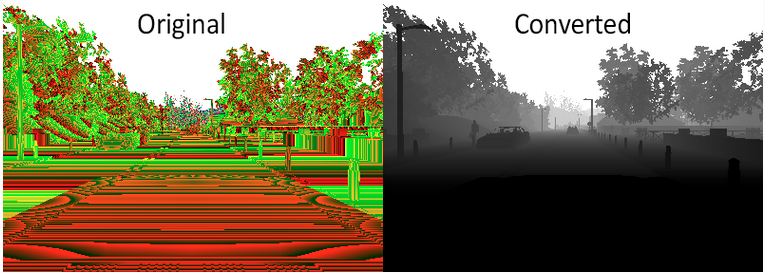
\includegraphics[width=0.75\textwidth]{pictures/depth_map_carla.png}
    \caption[CARLA Tiefenkarte]{Depth Map Pseudosensor des Simulators in Original und User freundlichen Konvertierung. (CARLA Dokumentation, 2022)}
  \end{center}
\end{figure}

Der Simulator verfügt viele, für autonomes Fahren relevante, Sensoren wie Kamera, Lidar, IMU, GNSS ect.. Die Sensoren werden über eine JSON-Konfigurationsdatei instanziiert und stehen immer in Relation zum Fahrzeug. Dabei sind alle Distanzen in Metern zu lesen.
\newline

Für die vorliegende Arbeit wurden zwei RGB Kamerasensoren zu einer Stereokamera konfiguriert und eine RGB Kamera mit Depth Map Sensor als RGB-D Kamera verwendet. Die Kameras müssen nicht rektifiziert werden und die intrinsischen (Kamera internen) Parameter sind direkt bekannt. Die Auswahl und Positionierung erfolgt über die CARLA API. Die Position wird dabei in Metern und immer in Bezug zum Fahrzeug definiert. Bilddaten werden vom Server als BGRA Bytearray gesendet.

Folgende Effekte aus dem Simulator haben Einfluss auf das Kamerabild:\\
\newline
\textit{Grain jitter} erzeugt ein künstliches Rauschen. \textit{Blooming} erzeugt eine helle Verzeichnung in der Umgebung einer Überbelichtung. \textit{Auto exposure} ändert den Bild-Gammawert, um Anpassung an dunklere oder hellere Bereiche zu simulieren. \textit{Lens flares} simuliert di Reflexion heller Objekte auf der Linse. \textit{Depth of field} lässt Objekte in der Nähe oder sehr weit von der Kamera unscharf werden. \newline


Unglücklicherweise werden diese Effekte über die Unreal Engine erzeugt und nicht in der Kamera in CARLA. Ein Blooming Effekt würde bei modernen CMOS beispielsweise i.d.R. nicht auftreten sondern ist ein CCD Phänomen. Auch die Implementierung des Auto-Exposure Effekts ist bei CARLA dem Menschlichen Auge nachempfunden um beim User einen besseres Optisches Erlebnis zu erzielen anstatt die Kamera korrekt zu modellieren.\newline


\subsection{Transformationsbaum}

\begin{figure}[h!]
  \centering
    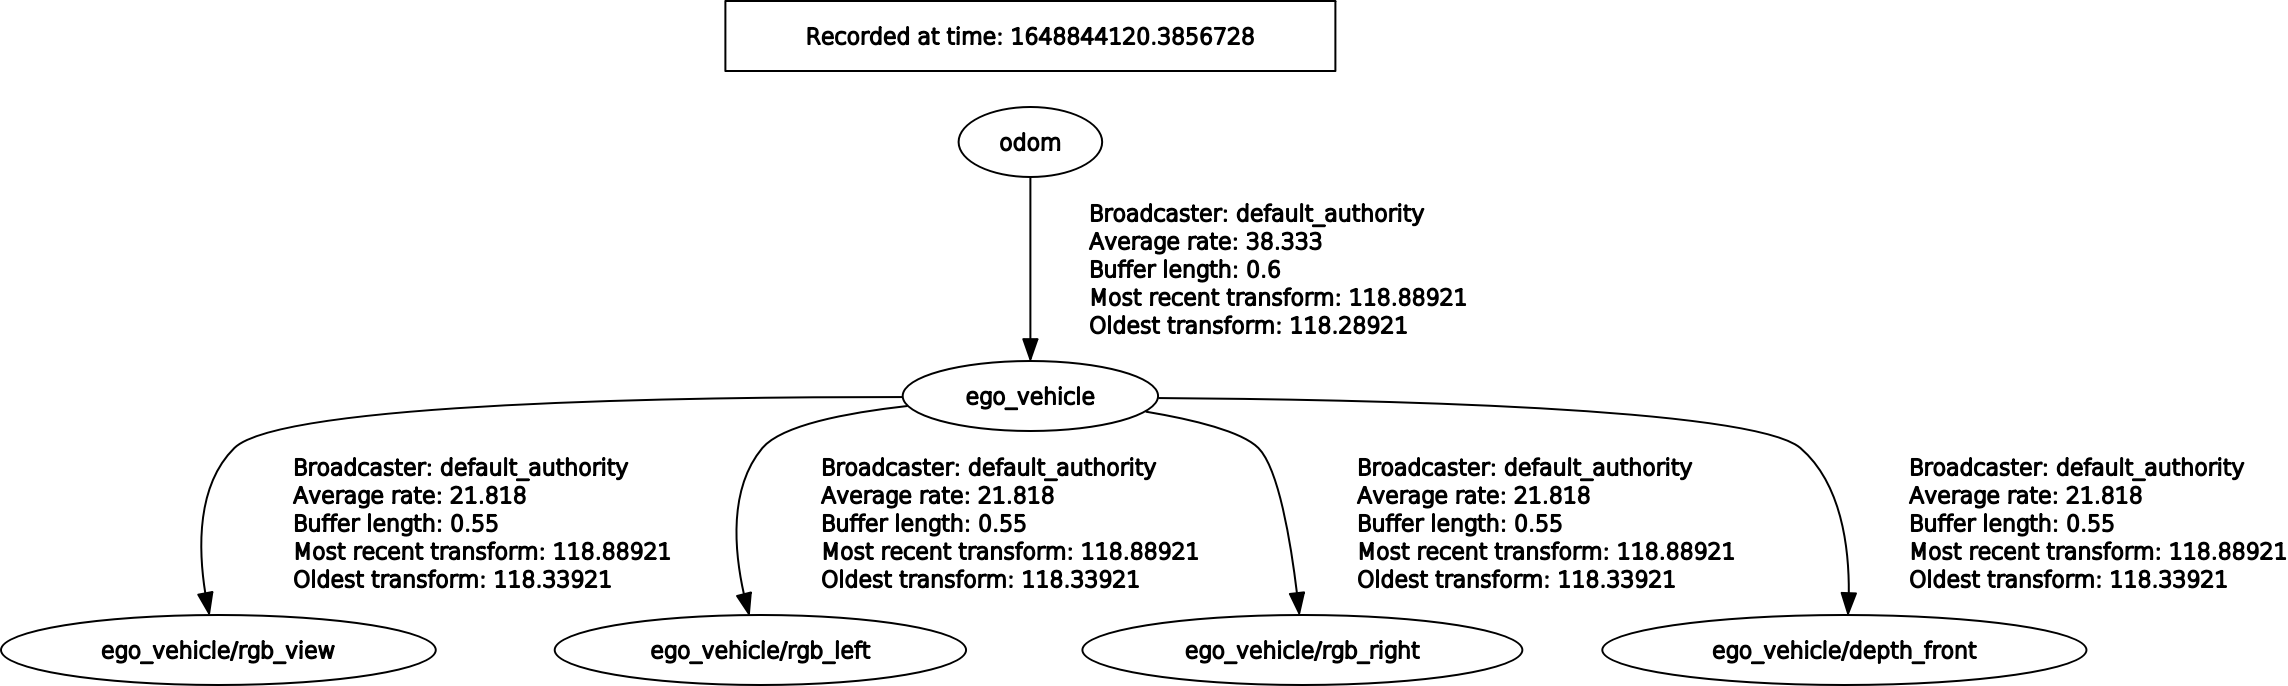
\includegraphics[width=0.75\textwidth]{pictures/05_tf_frames.png}
    \caption[ROS2 Transformationsbaum für Visuelle Odometrie]{ROS2 Transformationsbaum für den Versuchsaufbau.}
		\label{fig:tf}
\end{figure}

Im Netzwerk kann die räumliche Beziehung zwischen Nodes über einen Transformationsbaum abgebildet werden. Jeder Node hat sein eigenes Koordinatensystem. Über die Transformationen wird bekannt gegeben wie die Koordinatensysteme zu einander ausgerichtet sind. So kann beispielsweise definiert werden wo sich die Kameras in Bezug zum Mittelpunkt des Fahrzeugs befinden. Wird jetzt die Pose des Fahrzeugs aktualisiert, können auch alle Sensor Posen aktualisiert werden. 

Abbildung \ref{fig:tf} zeigt den Transformationsbaum des System. Neben den statischen Transformationen zwischen Sensoren und Fahrzeug (ego\_vehicle) ist auch die Transformation des Odometrie Frames zum Fahrzeug zu sehen. Wird das System in ein anderes Netzwerk eingebunden kann also über diesen Frame auf das Fahrzeug und alles was mit dem Fahrzeug verbunden ist lokalisiert werden.

\pagebreak
\section{Bibliotheken}

\subsection{Computer Vision Bibliothek OpenCV}

\begin{figure}[!h]
  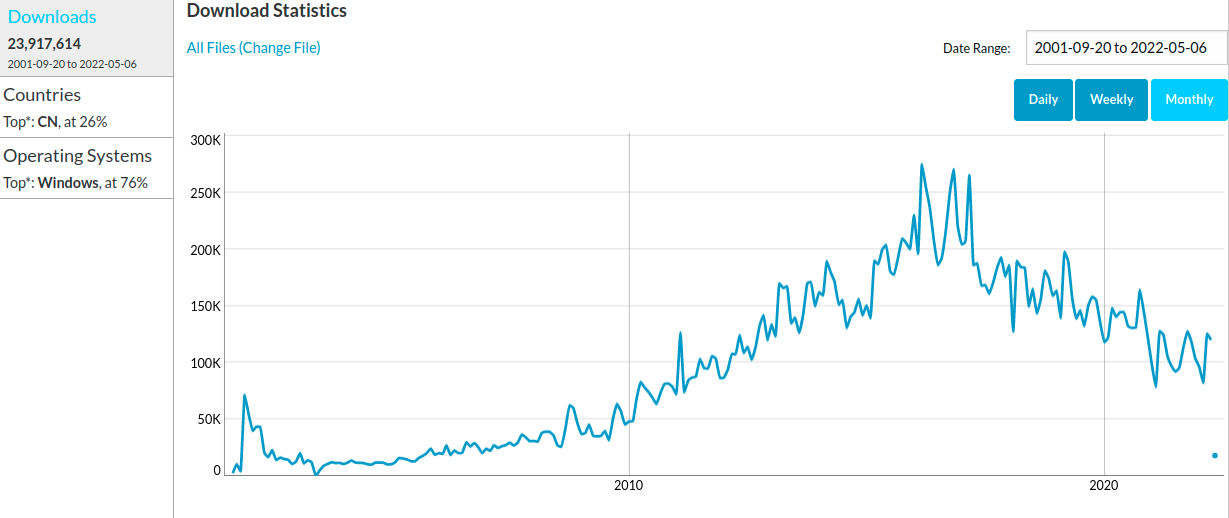
\includegraphics[width=0.9\textwidth]{pictures/06_cv_downloadstatistics.png}
  \caption[OpenCV Bibliothek Download Statistik]{SourceForge OpenCV Download Statistik zeigt über 23,9 Millionen Downloads seid dem 20.09.2001}
\end{figure}

Lokalisierung mittels Kameradaten ist ein bekanntes Problem der Bildverarbeitung. Über die Jahrzehnte sind viele Algorithmen und Funktionen entwickelt worden um die verschiedenen Aspekte der Problemstellung zu lösen. Über 2500 davon lassen sich in der Open Source Bibliothek OpenCV (Open Computer Vision) finden. OpenCV wurde ursprünglich von Intel entwickelt und hatte seine Erstveröffentlichung 2000. Der Fokus der Bibliothek liegt auf Echtzeit Bildverarbeitung. Viele Probleme der Bildverarbeitung sind äu{\ss}erst Rechenintensiv. Durch OpenCV sollen optimierte Implementierungen geschrieben werden und Robotik Ingenieure davon befreit 'das Rad neu erfinden zu müssen'.
\newline

OpenCV ist in C++ geschrieben bietet Interfaces in Python, Java, MATLAB und Mobile Device Ports. Durch die hohe Qualität der Bibliothek und die Fülle an Anwendungen der Bildverarbeitung wird OpenCV von sehr vielen Firmen und Forschungseinrichtungen benutzt wie beispielsweise Google, Microsoft, Sony, MIT, Intel, Siemens usw.. Die Zahl der Downloads liegt aktuell bei fast 24 Millionen.
\newline

Für den Systementwurf wurde OpenCV als Grundlage für das Prototyping verwendet. Die Bibliothek hat es ermöglicht einen schnellen praktischen Zugang zu der Theorie aus wissenschaftlichen Veröffentlichungen hinter der Bildverarbeitung zu erlangen. Stellenweise konnten Parameter für die VO heuristisch ermittelt werden und es erleichterte den Vergleich verschiedener Algorithmen.
\newline 

Neben der optimalen Implementierung von Algorithmen wird bei OpenCV auch an eigene Forschung zu neuen Methoden betrieben. Der im System verwendete ORB Algorithmus ist eine Eigenentwicklung der OpenCV Researcher. 
\newline

Alternativ zu OpenCV kann für das Prototyping beispielsweise MATLAB verwendet werden falls der Entwickler mit dieser Umgebung besser vertraut ist. Die Performance von MATLAB gegenüber OpenCV ist jedoch bis zu 80 mal langsamer \cite{cvmatlab}. Code der mit OpenCV geschrieben wurde kann zudem direkt auf dem Zielsystem laufen.

\subsection{V-SLAM Bibliothek RTAB-Map}
RTAB-Map ist eine standalone C++ Open Source Bibliothek für Real-Time Appearance Based Mapping. Unter der Verwendung von OpenCV werden RGB-D, Stereo and Lidar Graph-Based SLAM Algorithmen implementiert \cite{labbe}.
\newline

RTAB-Map wird auch als ROS und ROS2 Package veröffentlicht. Der ROS Philosophie folgend sind verschiedene Teiles der SLAM Algorithmen als Nodes implementiert, aus denen sich ein vollständiges SLAM zusammensetzt. Für Visual SLAM ist die visuelle Odometrie das Front-End zur Bildverarbeitung. Es gibt daher einen Stereo Odometrie Node aus RTAB-Map der zur Realisierung der visuellen Odometrie für die Fahrzeuge des CARS Projekt verwendet werden kann. \newline

Der Node hat eine Parameterliste von 242 Parametern die wie eine API für die unterliegenden Funktionen funktioniert. In den meisten Fällen sind die Parameter Übergabewerte an OpenCV Funktionen. Der Node bietet dadurch die Möglichkeit direkt eine VO Pipeline aufzurufen und sich vollständig auf die Parametrierung der CV Funktionen z.B. WindowSize der Merkmalsdetektoren zu konzentrieren.

\chapter{Ergebnisse der Lokalisierung}
\section{Methodik}
\begin{figure}{!ht}
	\centering
	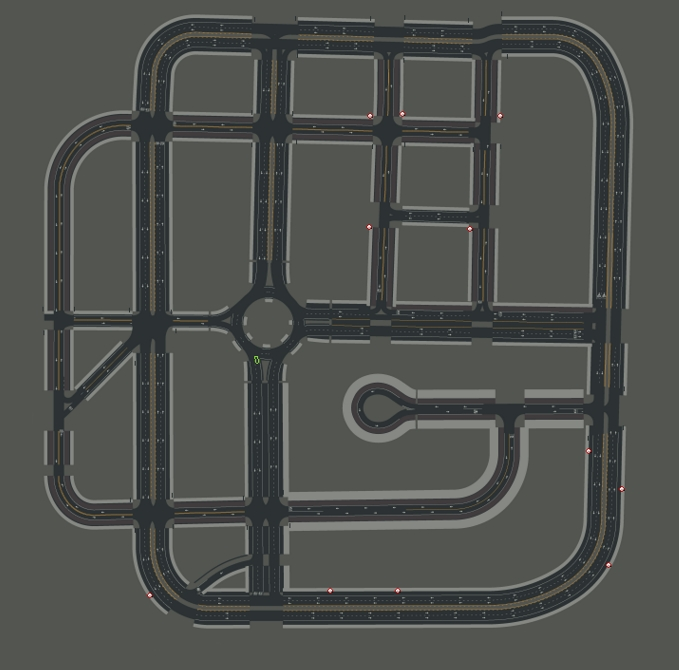
\includegraphics[width=0.45\textwidth]{07_Town03.jpg}
	\caption[CARLA Simulator Karte Town03]{CARLA Simulator Karte Town03. (CARLA Dokumentation, 2022)}
\end{figure}

Für die Datenerhebung wurde im CARLA Simulator die Umgebung 'Town03' ausgewählt. Die CARLA Dokumentation beschreibt Town03 als abwechslungsreichste und komplexeste Karte des Simulators. Town03 beinhaltet eine gro{\ss}e Kreuzung, Erhebungen, Kreisverkehr und einen Tunnel.
\newline

Es wurden Daten für 5 unterschiedliche Witterungsverhältnisse erhoben: sunset, clear night, default, hard rain, wet sunrise. Die Witterungsverhältnisse wurden über CARLAs Python API gesetzt.
\newline 

Für jedes Witterungsverhältnis wurden 5 Testfahrten aufgezeichnet. Die Testfahrten sind zufällige Strecken. Au{\ss}erdem wurden für alle Fahrten 50 NPCs auf der Karte gespawnt. NPC beinhalten andere Fahrzeuge sowie Fu{\ss}gänger. Die Geschwindigkeit des Testfahrzeugs variiert zwischen 30 und 100 $\frac{km}{h}$, je nach Streckenabschnitt.
\newline

Bei jeder Testfahrt waren die Stereokamera und die RGB-D Kamera am Fahrzeug angebracht, das Bild der linken RGB Kamera wurde in beiden verwendet. Die ROS Nodes für beide Visuellen Odometrie Programme laufen bei allen Fahrten live mit und alle Ausgangsdaten wurden über das ROS Werkzeug rosbag in eine sql3 Datenbank geschrieben.
\newline

Ein Verarbeitunsgtool 'BagParser' wurde geschrieben um Daten aus den rosbag Datenbanken zu extrahieren und in .txt Dateien, OpenCV Matritzen oder Quarternion formatierte .txt Dateien abzulegen. 
\newline

Die Bewertung von geschätzten Trajektorien bringt einige Herausforderungen mit sich. 

Zum einen referenzieren Ground Truth und die Schätzung unterschiedliche Koordinatensysteme. Ground Truth referenziert das Fahrzeugkoordinatensystem währen die VO Schätzung das Koordinatensystem der linken Kamera referenziert. Die Positionen müssen also zuerst aneinander angeglichen werden, bevor ein Vergleich durchgeführt werden kann. 
\newline

Ein anderes Problem ist die Fehlerfortpflanzung. Es kann sein, dass an einer Stelle ein Winkel mit gro{\ss}er Abweichung zu Ground Truth geschätzt wurde. Folgende Schätzungen sind vielleicht mit wesentlich kleineren Fehlern behaftet, zeigen im absoluten Vergleich aber noch den vorherigen Fehler. 

Es handelt sich bei den Daten au{\ss}erdem um hochdimensionale Datensätze; die Anzahl der Merkmale ist höher als die Anzahl der Beobachtungen.
\newline

Um mit diesen Herausforderungen umzugehen wurden die Daten basierend auf dem Paper \textit{Rethinking Trajectory Evaluation for SLAM: a Probabilistic, Continuous-Time Approach}\cite{zhangSLAM} und der Trajectory Evaluation Toolbox aus \textit{A Tutorial on Quantitative Trajectory Evaluation for Visual(-Inertial) Odometry} \cite{errorEst} bewertet.
\newline

Voraussetzung für eine Evaluation ist zuerst die gleiche Ausrichtung der geschätzten Trajektorien mit Ground Truth. Die beiden sind durch eine euklidische Transformation im 3 Dimensionalen Raum miteinander verbunden. Die Transformationen bestehen aus Rotation und Translation und werden Formal als Spezielle Euklidische Transformation SE(3) bezeichnet. Anstatt mit Rotationsmatritzen zu rechnen werden für die Auswertung mit rotations Quaternionen gerechnet. Quaternionen sind ein eigener Zahlenbereich und eine Erweiterung des Zahlenbereichs der reellen Zahlen. Als Vorbereitung der Auswertung müssen die Trajektorien daher als Messreihe von 7-Dimensionalen Vektoren abgelegt werden 
\begin{equation}
	\centering
		X_i = (x\; y\; z\; q_w\; q_x\; q_y\; q_z)^\top 
\end{equation}

Die Ausrichtung wird durch eine Methode der Kleinsten Quadrate Implementation für zwei Punktmengen nach Umeyama \cite{Umeyama1991LeastSquaresEO} gelöst.

\begin{equation}
	\centering
	\underset{R,T,s}{\arg\min} \sum_{i = 0}^{N} \| \hat{t}_i -sR_{ti} -T \|^2   
\end{equation}

Mit Ground Truth Posen als $\hat{t}$ und Schätzung durch Visuelle Odometrie als $s$. 
\newline

In der Auswertung werden für jede Strecke der absolute Streckenfehler ATE (Absolute Trajectory Error) und der relative Fehler (RE) berechnet. Ground Truth sei $X_{gt}$ und die, bereits ausgerichtete, geschätzt Trajektorie sei $\hat{X}'$. Die Trajektorie ist der zeitlicher Verlauf der Zustände der VO Schätzung. Für einen einzelnen Zustand wird der Fehler zwischen $\hat{x}'_i$ und Ground Truth $x_i$ definiert als  
\begin{equation}
	\Delta x_i = \{\Delta R_i, \Delta p_i\}
\end{equation}
für die gilt
\begin{equation*}
	R_i = \Delta R_i \hat{R}'_i,\:
	p_i = \Delta R_i \hat{p}'_i	
\end{equation*}

mit der Rotationsmatrix $R$ und der Position $p$. Dadurch errechnet sich der absolute Fehler zu 

\begin{align}
	\Delta R_i &= R_i (\hat{R}'_i)^\top,\\
	\Delta p_i &= p_i - \Delta R_i \hat{p}'_i
	\label{eq:absoluteErr}
\end{align}

Nun kann, um den die Qualität der Gesamtstrecke zu quantifizieren, die Quadratwurzel des mittleren quadratischen Fehlers (root mean square error (RMSE)) gebildet werden
\begin{align}
	ATE_{rot} &= (\frac{1}{N} \sum_{i = 0}^{N-1} \|\angle (\Delta R_i)  \|^2 )^\frac{1}{2},\\
	ATE_{pos} &= (\frac{1}{N} \sum_{i = 0}^{N-1} \| (\Delta p_i)  \|^2 )^\frac{1}{2}
\end{align}

wobei $\angle(\cdot)$ für die Konvertierung der Schreibweise von Matrixform zu Euler-Winkel.
\newline
\newline

Zusätzlich wird der relative Fehler berechnet. Der von Zhang et al. \cite{errorEst} vorgeschlagene Ansatz ist, die relative Beziehung zwischen den Zuständen zu verschiedenen Zeiten zu messen. Das gemeinsame Kriterium der Zustände ist die zurückgelegte Distanz. Es wird also die Gesamtstrecke und die Schätzung der Gesamten Stecke in Teilstrecken $s$ und $e$ für den Abschnitt $\mathfrak{F}$ zerlegt. 
\newline

Für jeden Teilabschnitt werden aus den Messwerten Gruppen mit $K$ Zustandspaaren zusammengefasst. Die Menge der Paare $d_k$ bilden jeweils eine Trajektorie für den Streckenabschnitt $\mathfrak{F}$. 

\begin{equation}
	\mathfrak{F} = \{d_k\}^{K-1}_{k=0}, \:\:\: d_k= \{ \hat{x}_s, \hat{x}_e
\end{equation}

Der relative Fehler $\delta d_k$ berechnet sich auf die gleiche Weise wie der absolute Fehler \ref{eq:absoluteErr}. Somit ergibt sich der Fehler $\delta d_k$  für ein Wertepaar $d_k$ aus

\begin{align}
	\delta \phi_k & = \angle \delta R_k = \angle R_e(\hat{R'_e})^\top,\\
	\delta p_k &= ||p_e - \delta R_k \hat{p}'_e||^2.
\end{align}

Daraus ergibt sich eine Menge von Werten, jeweils einer pro Teilabschnitt. Die Menge wird formal beschrieben durch 

\begin{align}
	RE_{rot} \: &= \: \{\delta \phi_k\}^{K-1}_{k=0},\\
	RE_{pos} \: &= \: \{\delta p_k\}^{K-1}_{k=0},\\
\end{align}

Die Abbildung dieser Mengen ist in den Boxplots zu sehen. Der mittlere Kasten besteht aus zwei Quartilen und dem Median. Der Median ist der Strich, die Quartile beinhalten sämtliche Schätzfehler. Die Antennen bzw Whiskers bilden das obere und untere Quartil.

\newpage
\section{Ergebnisse}
%%%%%%%%%%%%%%%%%%%%%%%%%%%
\begin{figure}[!ht]
	\centering
	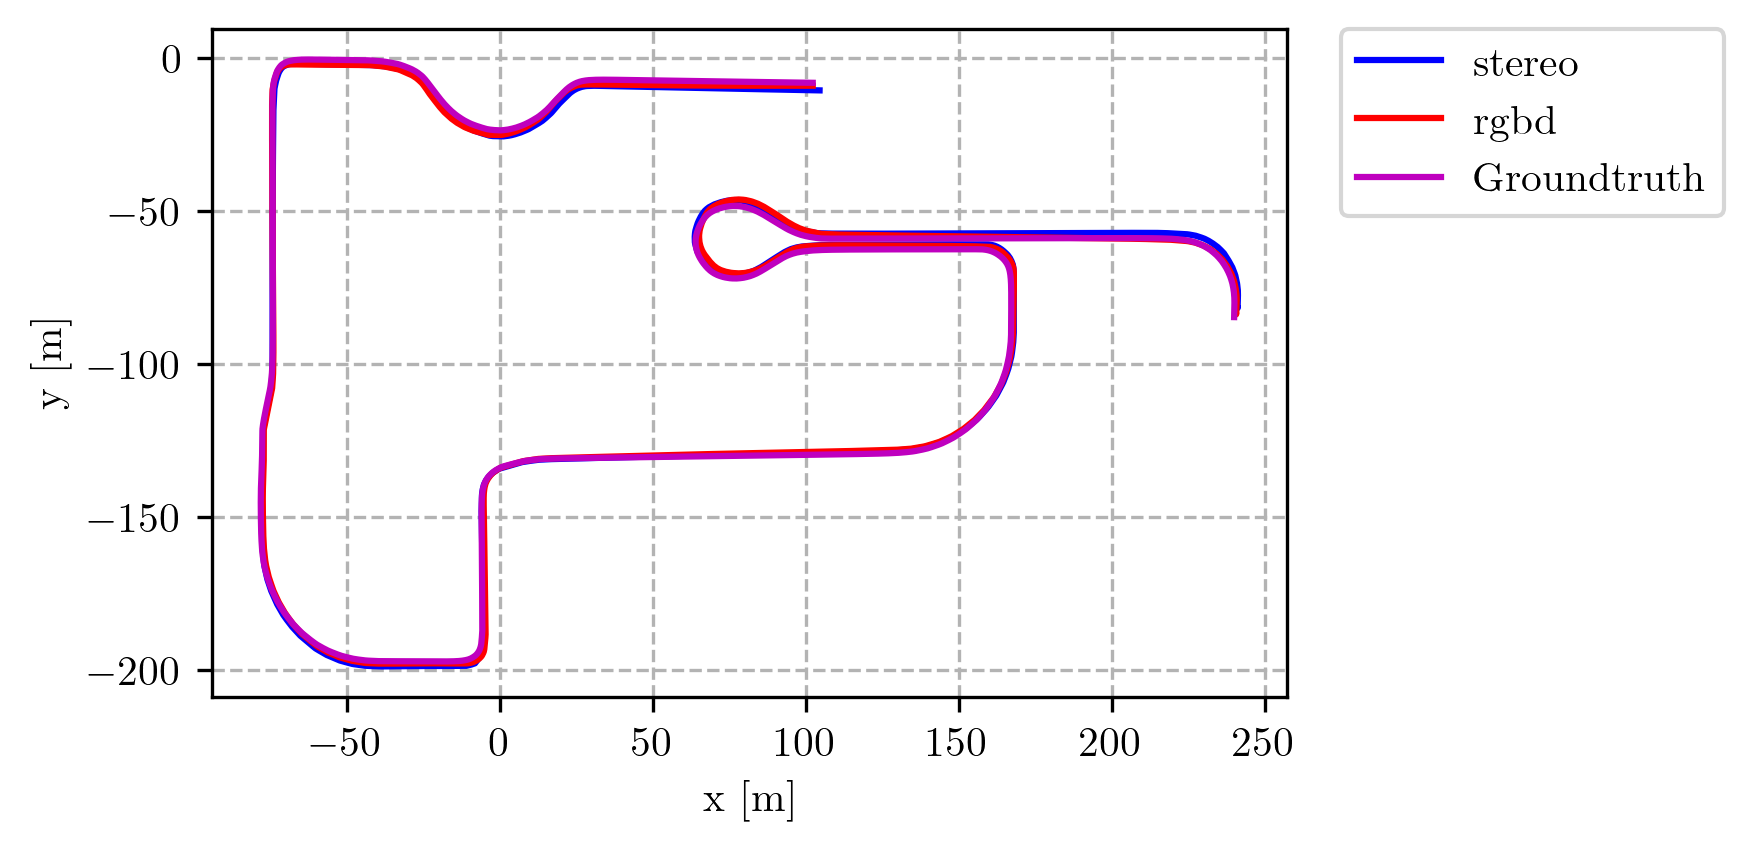
\includegraphics[width=\textwidth]{vorzeigestrecke/default_01_trajectory_top.png}
	\caption[Plot der Trajektorien Teststrecke 'Default 01']{Trajektorien Ground Truth und Schätzung durch Visuelle Odometrie der Teststrecke 'Default 01'}
\end{figure}

Es wurden insgesamt Daten für 25 Testfahrten erhoben. Der Datensatz einer Testfahrt besteht immer aus den Ground Truth Odometrie Daten, der durch RGB-D geschätzten Odometrie und der durch Stereo geschätzten Odometrie. Zugunsten der Übersichtlichkeit werden nicht alle Strecken und Daten grafisch aufbereitet. Stattdessen wurden Daten einzelner Strecken als Stichproben abgebildet um einen intuitiven Einblick in die Ergebnisse zu vermitteln. 

	\begin{figure}[!ht]
	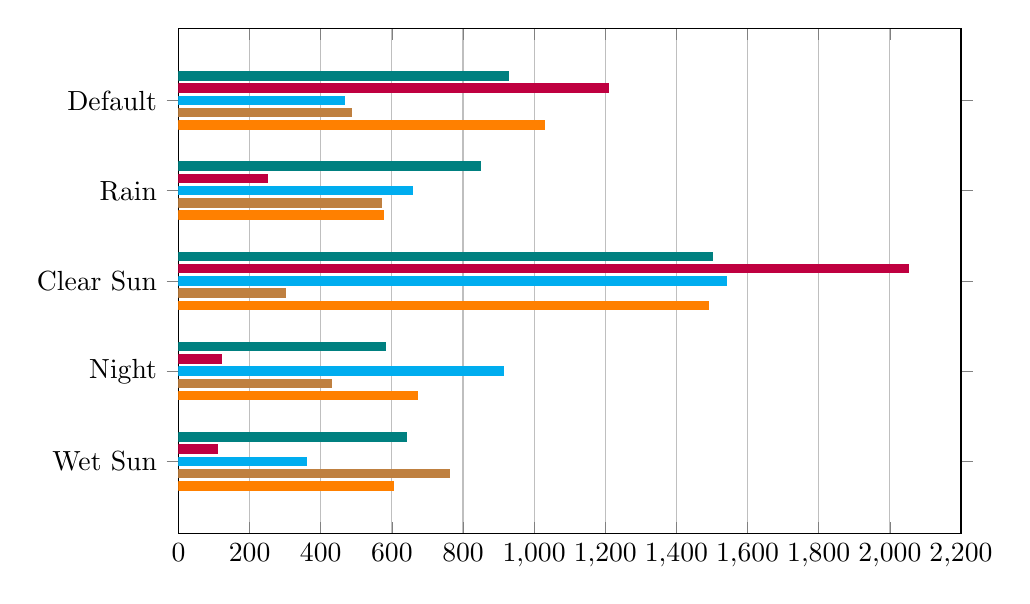
\begin{tikzpicture}
  \begin{axis}
      [
        width  = .95\textwidth,
        height = 8cm,
        xbar = .05cm,
        bar width=3pt,
        xmajorgrids = true,
        xmin = 0, 
        xmax = 2200,
        ytick=data,
        %enlarge x limits = {value = .25, upper},
        enlarge y limits = {abs = .8},
        yticklabels={Wet Sun, Night, Clear Sun, Rain, Default}
      ]
      %Run 1 bei allen
      \addplot[xbar][style={orange,fill=orange,mark=none}]
      coordinates {(604,0) (672,1) (1491,2) (575,3) (1029,4)};
      %Run 2 bei allen
      \addplot[xbar][style={brown,fill=brown,mark=none}]
      coordinates {(763,0) (429,1) (301,2) (571,3) (486,4)};
      %Run 3 bei allen
      \addplot[xbar][style={cyan,fill=cyan,mark=none}]
      coordinates {(359,0) (915,1) (1540,2) (658,3) (466,4)};
      %Run 4 bei allen
      \addplot[xbar][style={purple,fill=purple,mark=none}]
      coordinates {(109,0) (121,1) (2052,2) (249,3) (1208,4)};
      %Run 5 bei allen
      \addplot[xbar][style={teal,fill=teal,mark=none}]
      coordinates {(641,0) (582,1) (1500,2) (850,3) (929,4)};
  \end{axis}
\end{tikzpicture}
	\caption[Testfahrten Streckenlängen]{Streckenlängen aller 25 Testfahrten in m.}
\end{figure}

Die Datensätze Simulieren unterschiedliche Sichtverhältnisse. Es sei angemerkt das die Fahrzeuge im CARLA Simulator über keine eigenen Lichtquellen verfügen.

\begin{figure}[!ht]
	\begin{tabular}{lll}
		1 & 	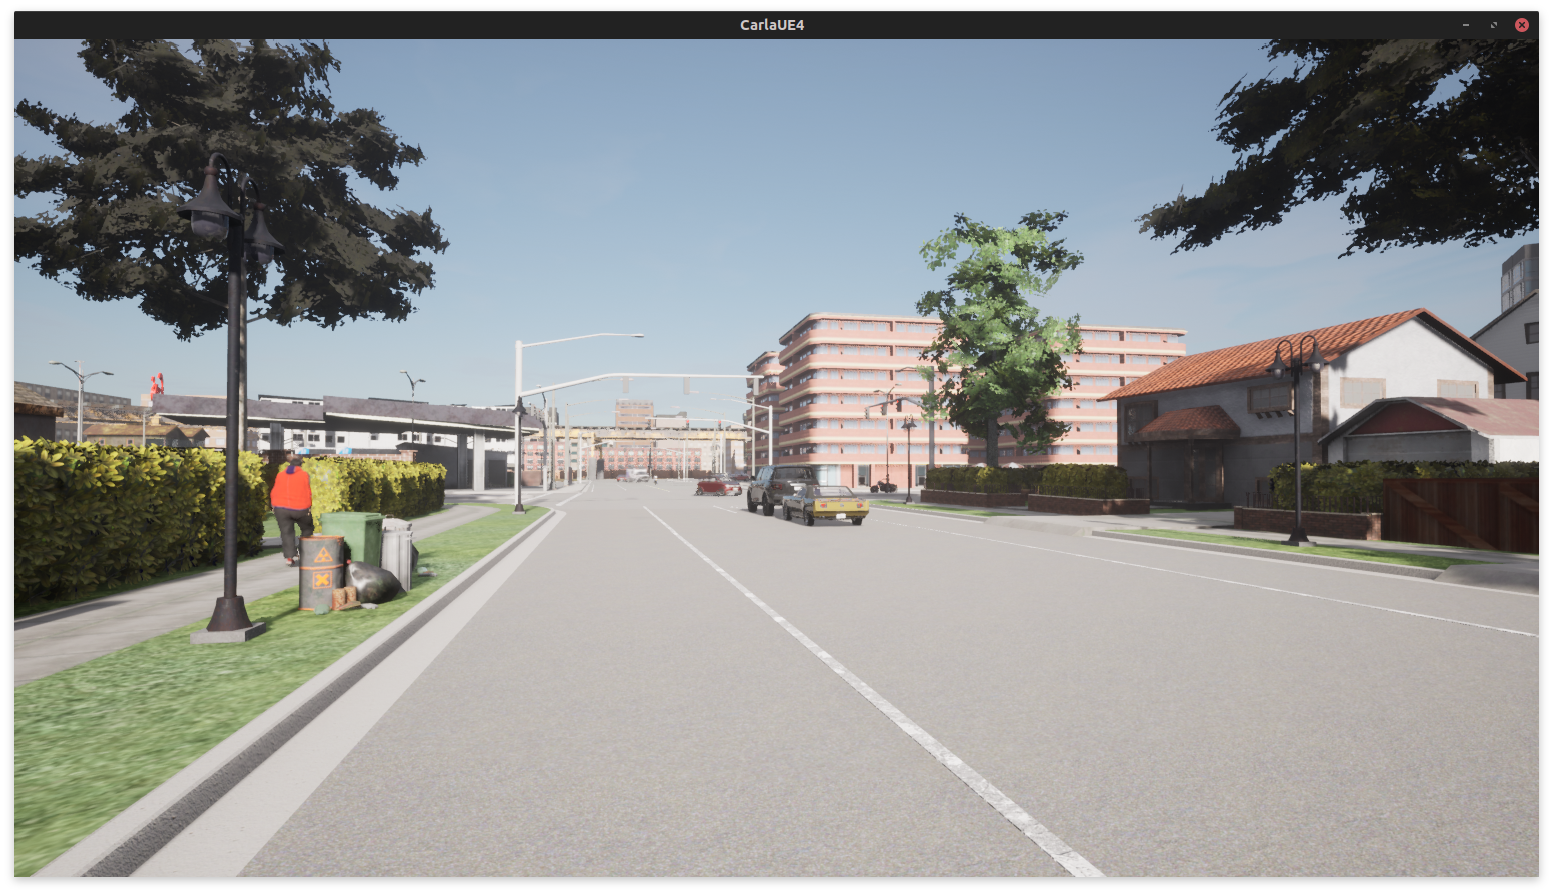
\includegraphics[width=.4\textwidth]{07_default.png} &
		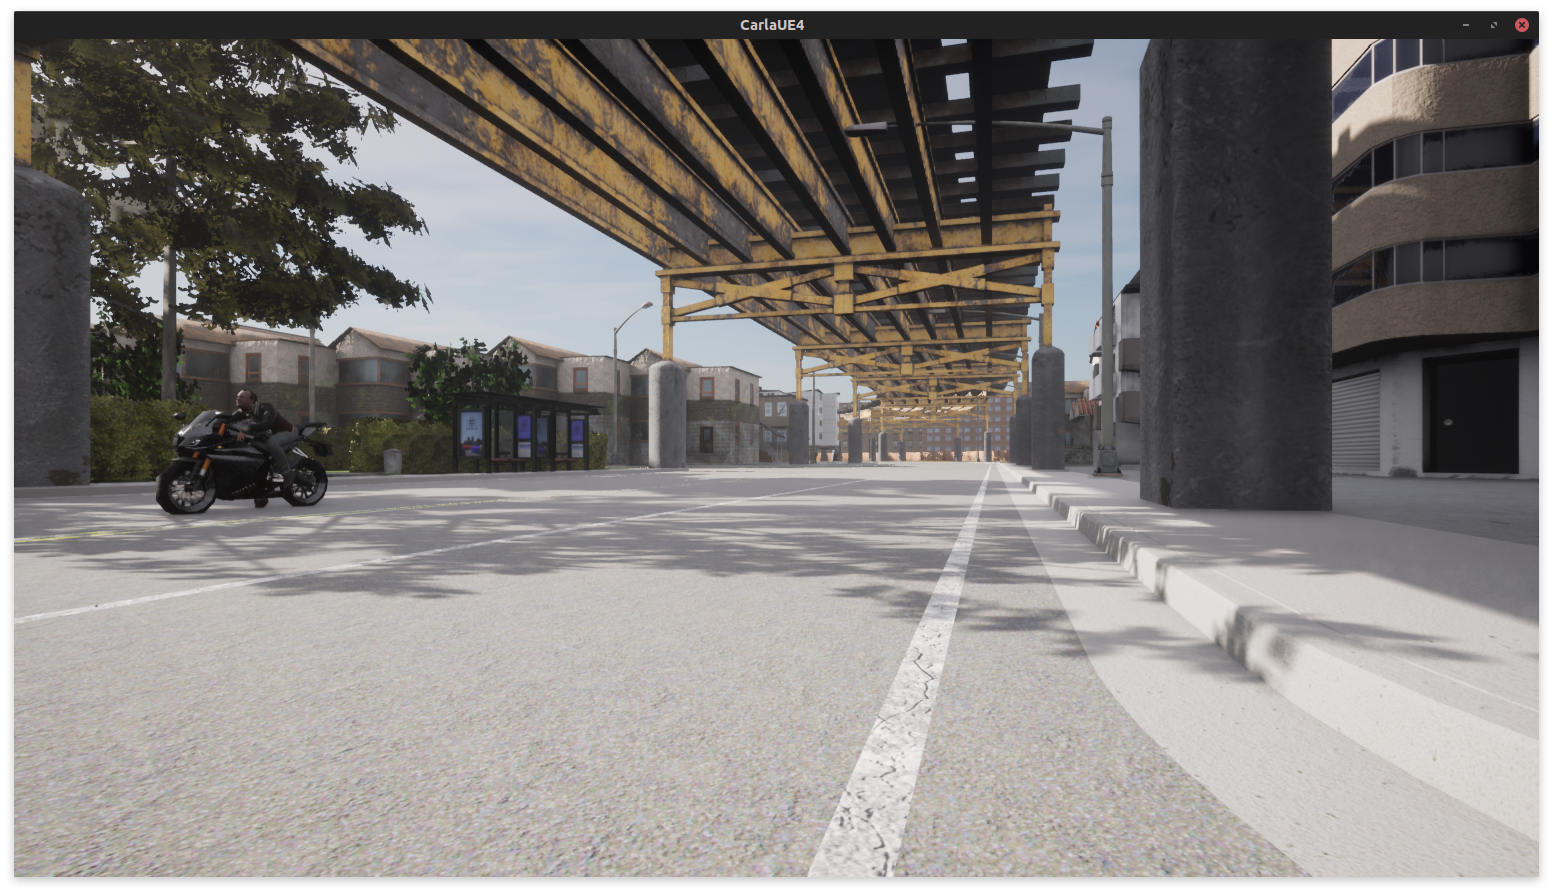
\includegraphics[width=.4\textwidth]{07_default03.png}\\
		2 & 	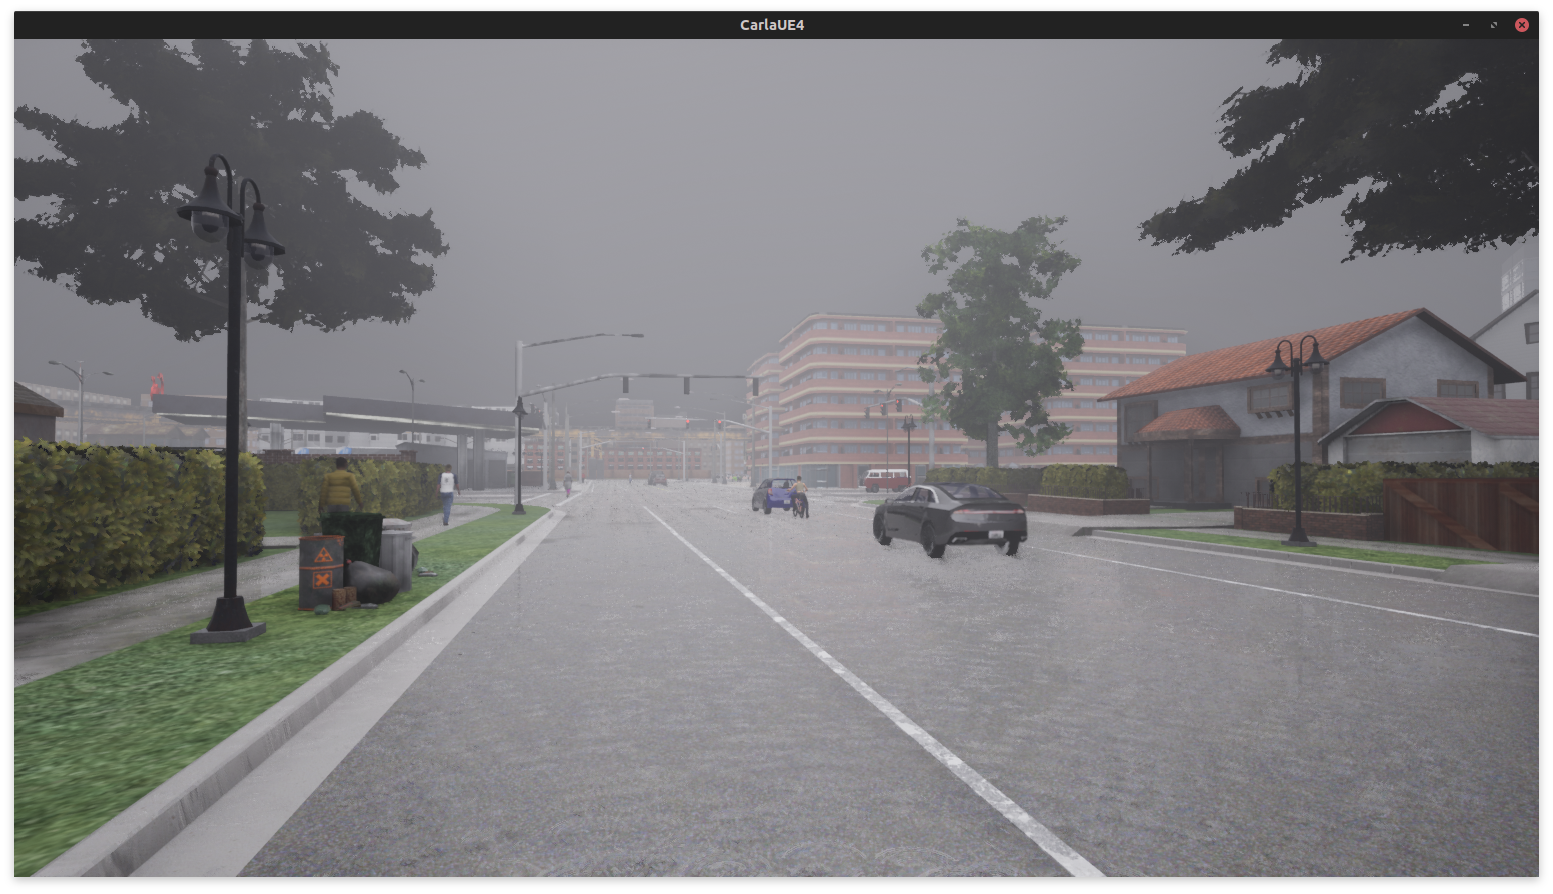
\includegraphics[width=.4\textwidth]{07_hard_rain.png} &
		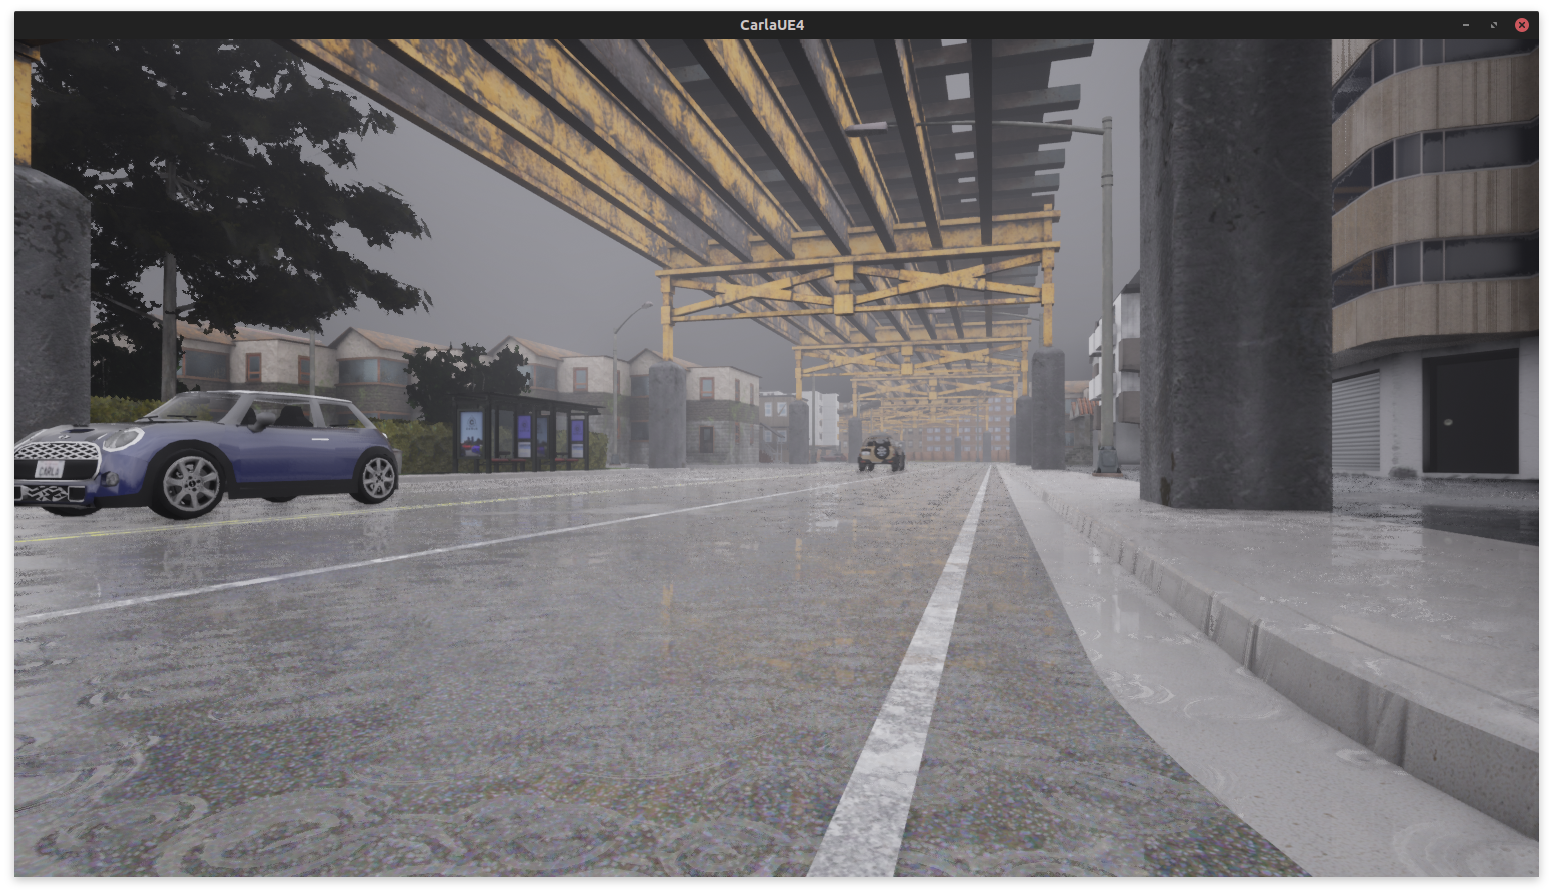
\includegraphics[width=.4\textwidth]{07_rain_noon03.png}\\
		3 & 	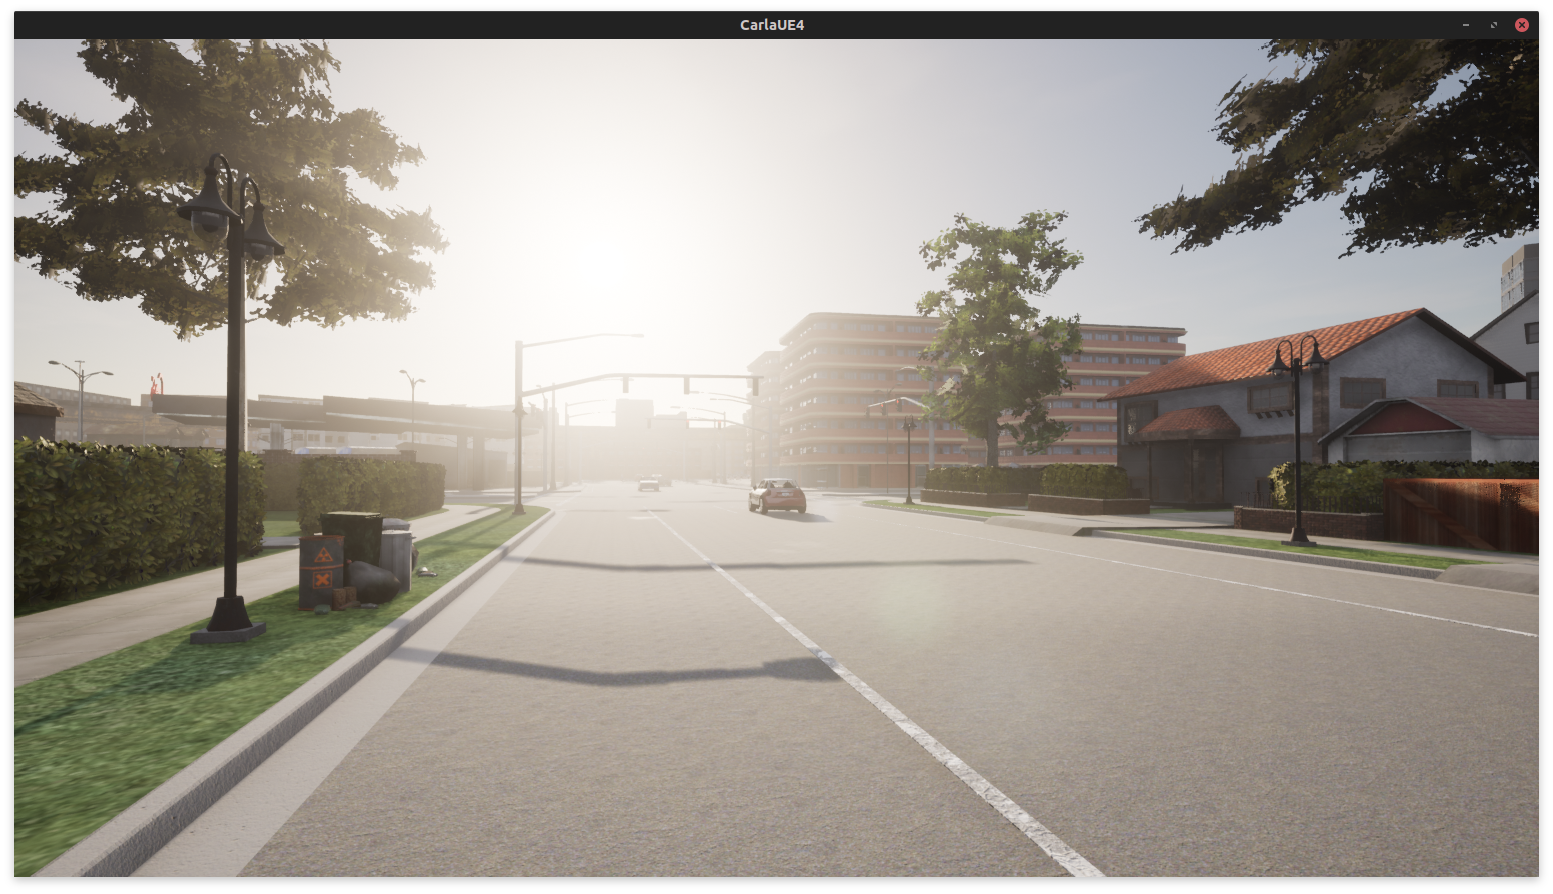
\includegraphics[width=.4\textwidth]{07_sunset.png} &
		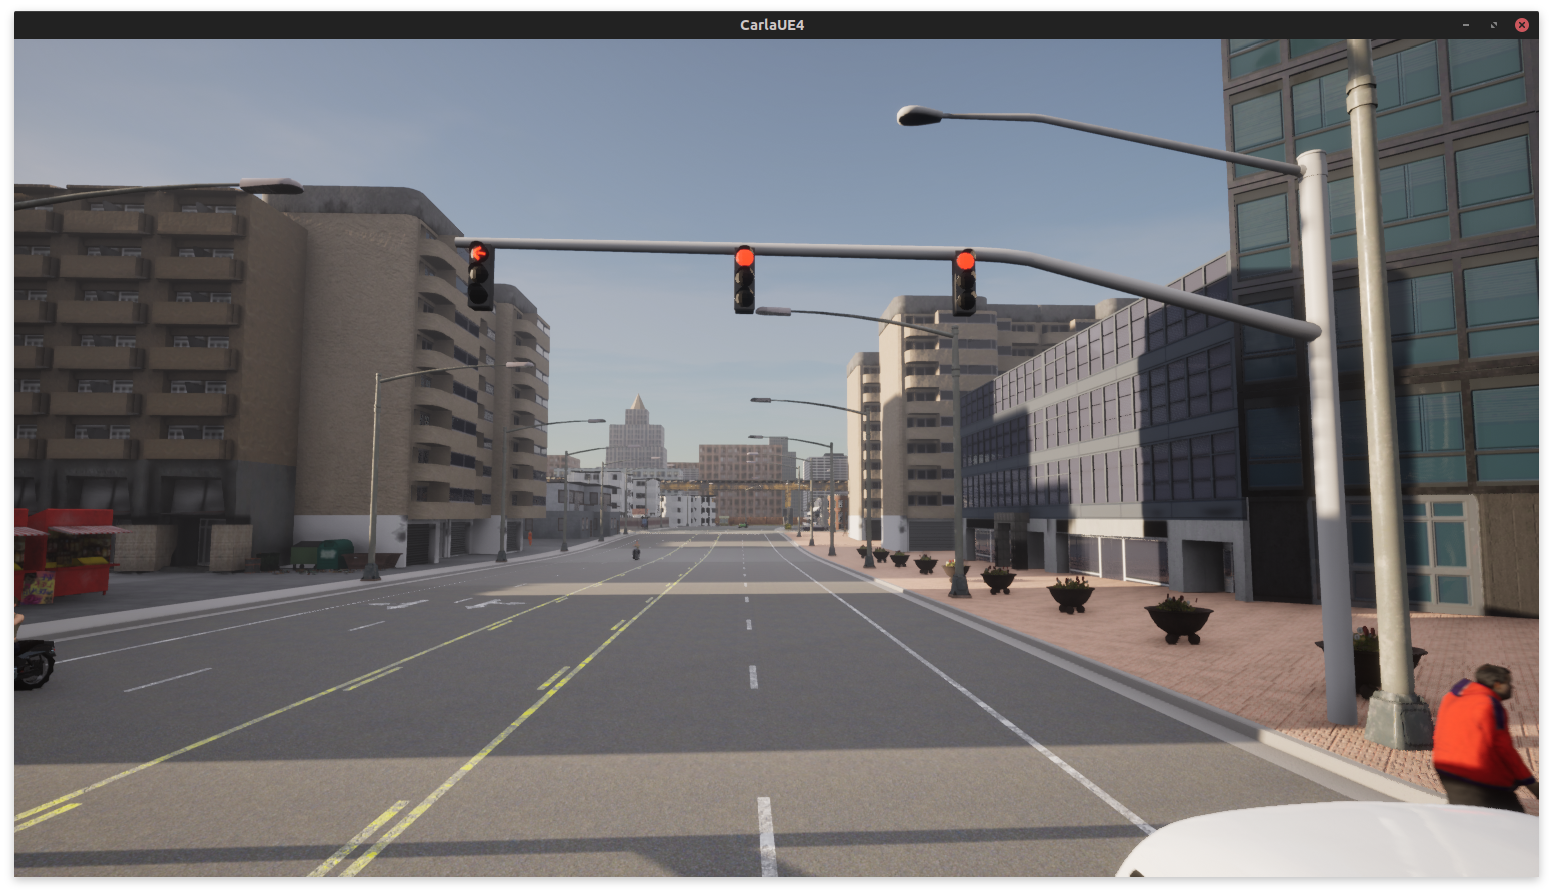
\includegraphics[width=.4\textwidth]{07_clear_sunset2.png}\\
		4 & 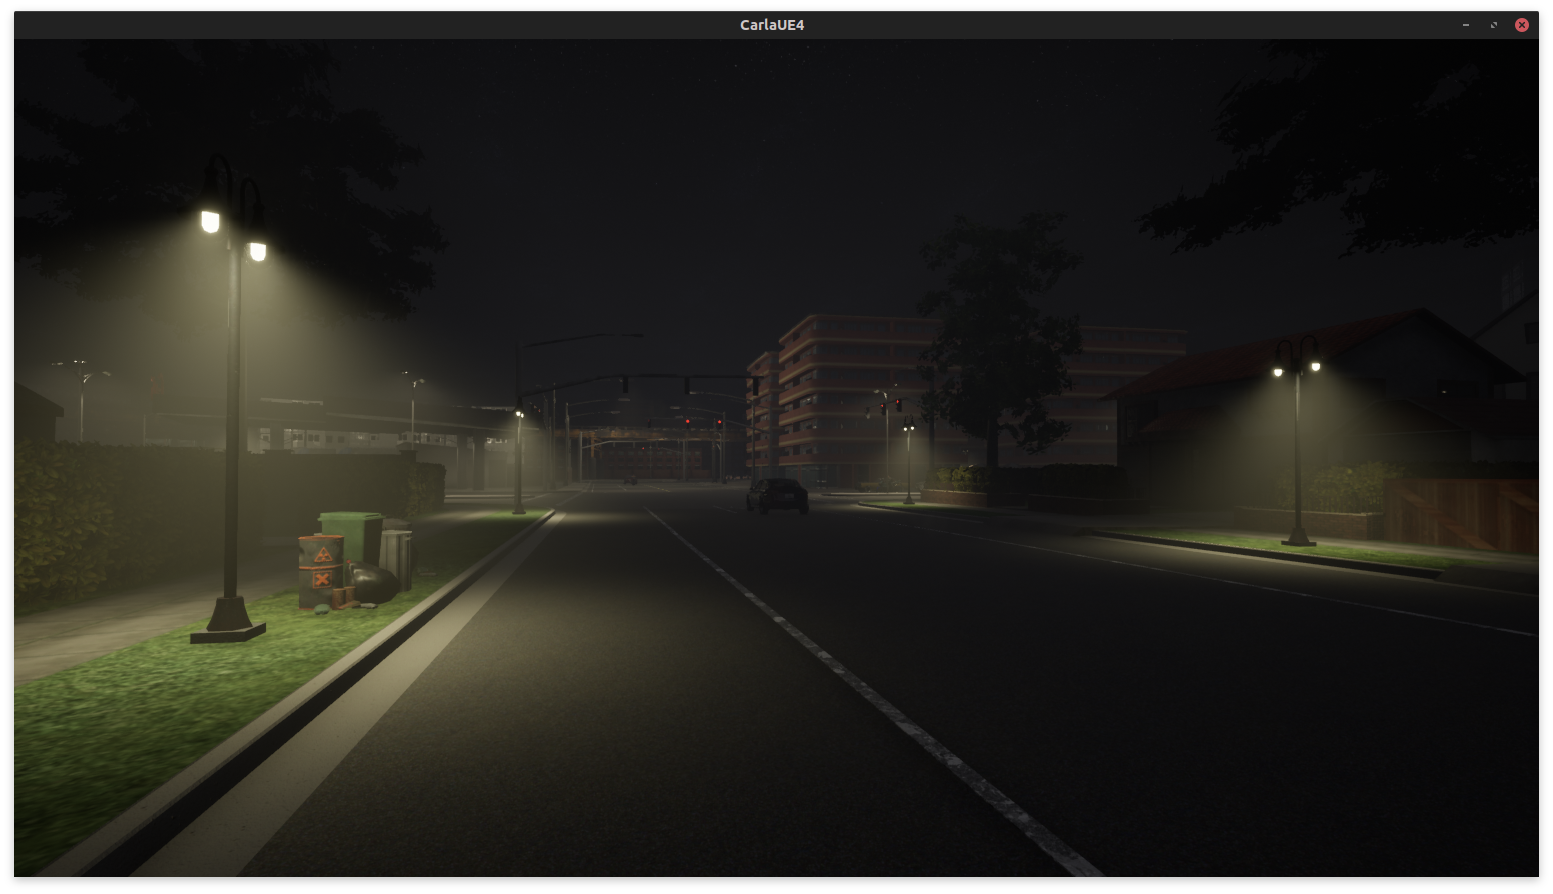
\includegraphics[width=.4\textwidth]{07_clear_night.png} &
		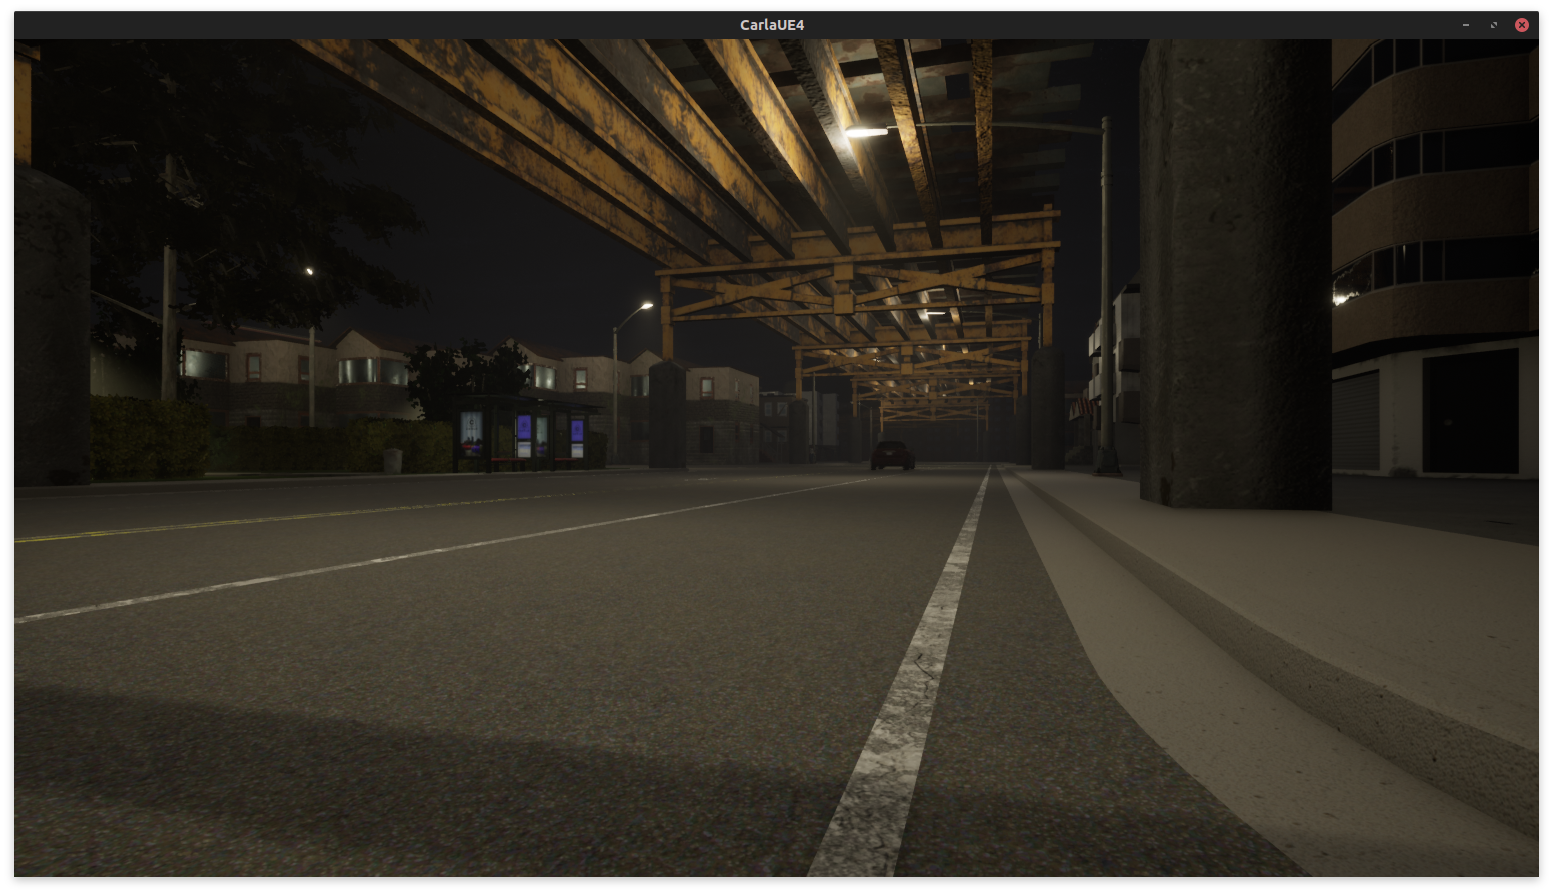
\includegraphics[width=.4\textwidth]{07_clear_night03.png}\\
		5 & 	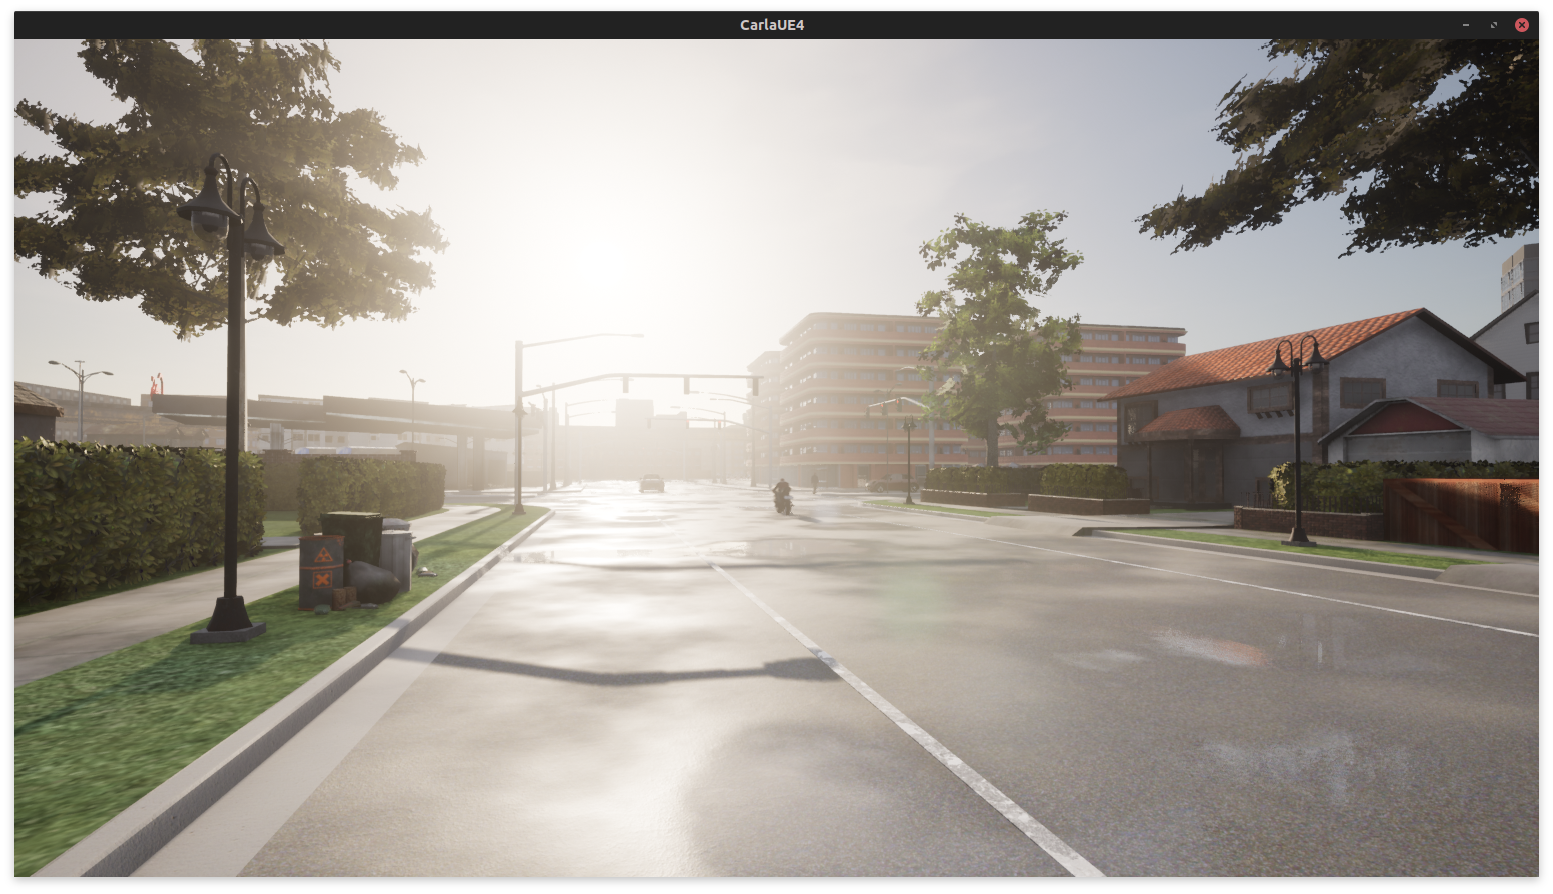
\includegraphics[width=.4\textwidth]{07_wet_sunset.png} &
		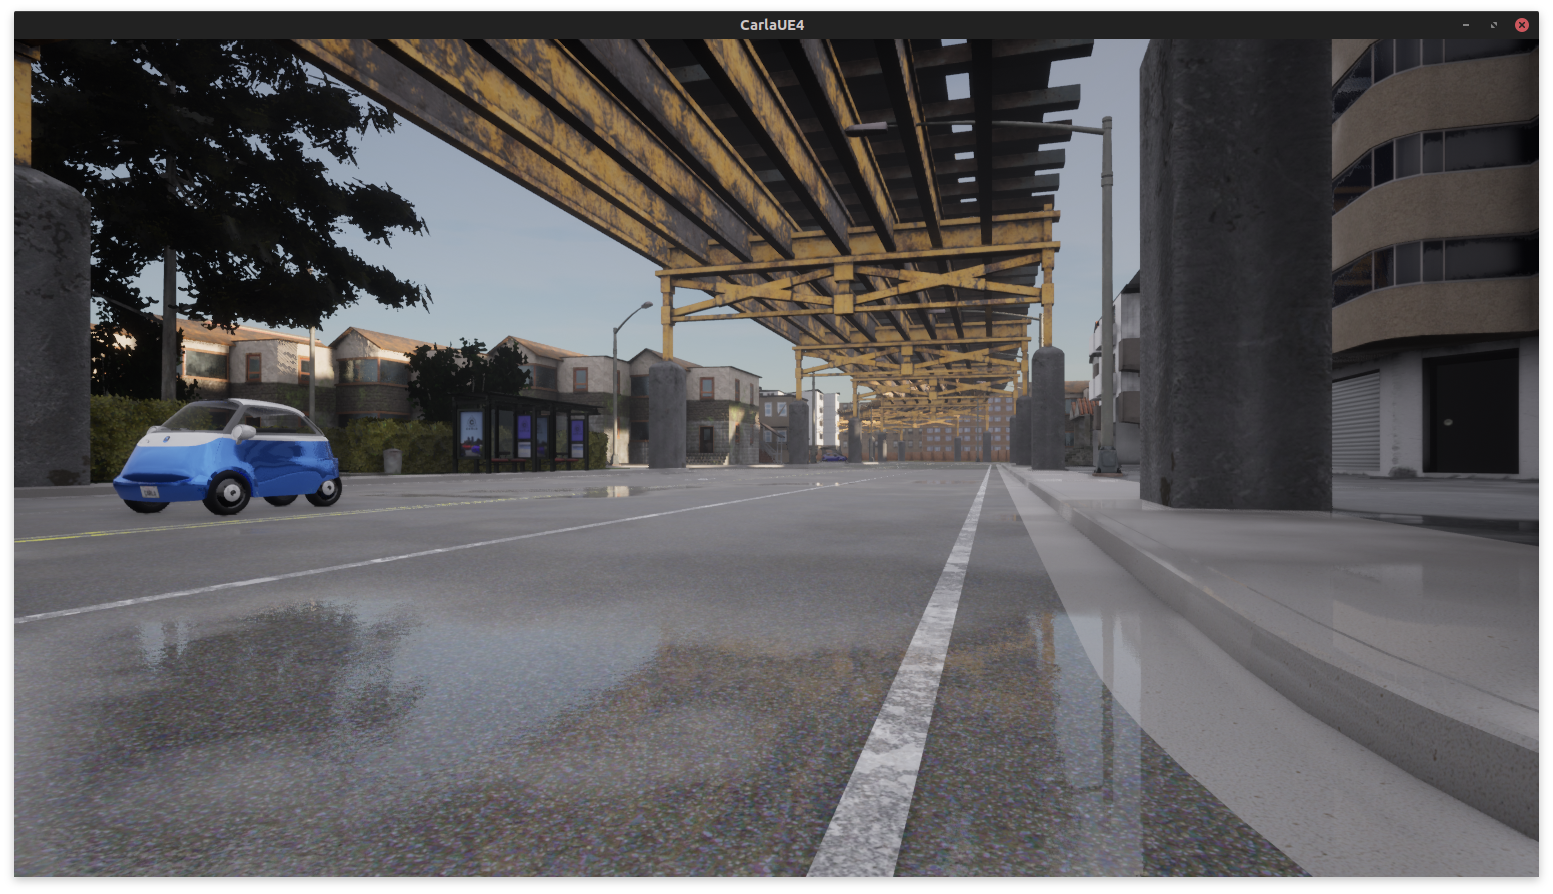
\includegraphics[width=.4\textwidth]{07_wet_sunset03.png}
		\end{tabular}
	\centering
	\caption[Witterungsverhältnisse der Simulation in verschiedenen Datensätzen]{Witterungsverhältnisse der verschiedenen Datensätze: 1 Default, 2 hard rain, 3 clear sunset, 4 clear night, 5 wet sunset}
	\label{fig:carlawetter}
\end{figure}


\newpage
\begin{figure}[!ht]
	% STEREO
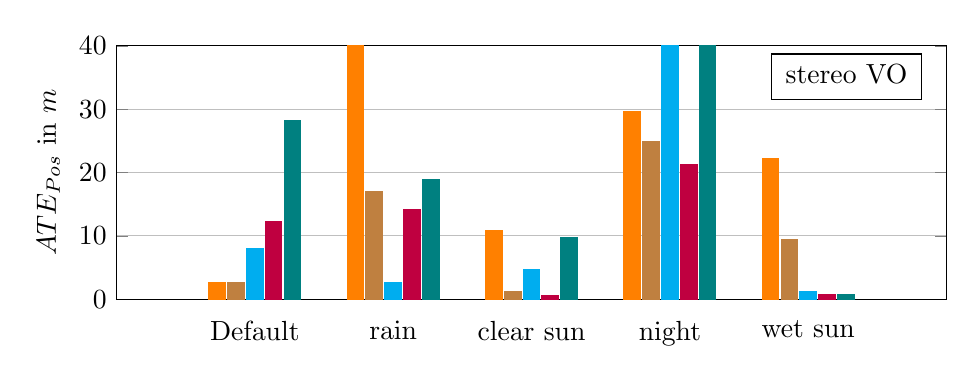
\begin{tikzpicture}
    \begin{axis}[
        width  = \textwidth,
        height = 4.8cm,
        ymax =40,
        major x tick style = transparent,
        ybar=2*\pgflinewidth,
        bar width=6pt,
        ymajorgrids = true,
        ylabel = {$ATE_{Pos}$ in $m$},
        % xlabel = {1 Default, 2 hard rain, 3 clear sunset, 4 clear night ,5 wet sunset},
        symbolic x coords={Default, rain, clear sun, night ,wet sun},
        xtick = data,
        scaled y ticks = false,
        enlarge x limits=0.25,
        ymin=0,
        legend pos=north east
    ]
    \addlegendimage{empty legend}
    \addlegendentry{stereo VO}
    \addplot[style={orange,fill=orange,mark=none}]
        coordinates {(Default, 2.70) (rain,66.61) (clear sun, 10.79) (night ,29.61) (wet sun, 22.271)};
    
    \addplot[style={brown,fill=brown,mark=none}]
        coordinates {(Default, 2.68) (rain,16.94) (clear sun, 1.16) (night , 24.96) (wet sun, 9.48)};
    
    \addplot[style={cyan,fill=cyan,mark=none}]
        coordinates {(Default, 8.07) (rain,2.663) (clear sun, 4.63) (night , 86.94) (wet sun, 1.29)};
    
    \addplot[style={purple,fill=purple,mark=none}]
        coordinates {(Default, 12.2) (rain,14.13) (clear sun, 0.569) (night ,21.32) (wet sun, .7)};
    
    \addplot[style={teal,fill=teal,mark=none}]
        coordinates {(Default, 28.2) (rain,18.87) (clear sun, 9.78) (night ,91.45) (wet sun, .7)};
    \end{axis}
  \end{tikzpicture}
	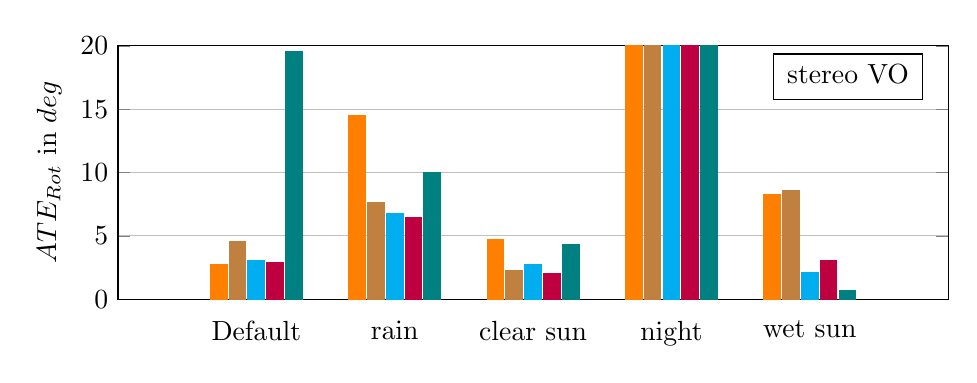
\begin{tikzpicture}
    \begin{axis}[
        width  = \textwidth,
        height = 4.8cm,
        ymax = 20,
        major x tick style = transparent,
        ybar=2*\pgflinewidth,
        bar width=6pt,
        ymajorgrids = true,
        ylabel = {$ATE_{Rot}$ in $deg$},
        % xlabel = {1 Default, 2 hard rain, 3 clear sunset, 4 clear night ,5 wet sunset},
        symbolic x coords={Default, rain, clear sun, night ,wet sun},
        xtick = data,
        scaled y ticks = false,
        enlarge x limits=0.25,
        ymin=0,
        legend pos=north east
    ]
    \addlegendimage{empty legend}
    \addlegendentry{stereo VO}
    \addplot[style={orange,fill=orange,mark=none}]
        coordinates {(Default, 2.73) (rain,14.53) (clear sun, 4.7107) (night ,44.90) (wet sun, 8.24)};
    
    \addplot[style={brown,fill=brown,mark=none}]
        coordinates {(Default, 4.52) (rain,7.65) (clear sun, 2.2452) (night ,20.45) (wet sun, 8.57)};
    
    \addplot[style={cyan,fill=cyan,mark=none}]
        coordinates {(Default, 3.05) (rain,6.74) (clear sun, 2.72) (night ,52.73) (wet sun, 2.11)};
    
    \addplot[style={purple,fill=purple,mark=none}]
        coordinates {(Default, 2.90) (rain,6.43) (clear sun, 1.99) (night , 58.59) (wet sun, 3.06)};
    
    \addplot[style={teal,fill=teal,mark=none}]
        coordinates {(Default, 19.58) (rain,9.99) (clear sun, 4.28) (night , 168.59) (wet sun, 0.672)};
    \end{axis}
  \end{tikzpicture}
	\caption[Absolute Trajectory Error (ATE) für Stereokamera]{Absolute Trajectory Error (ATE) für Stereo VO der geschätzten Translation und des geschätzten Winkels in Grad für alle 25 Testfahrten.}
	% STEREO
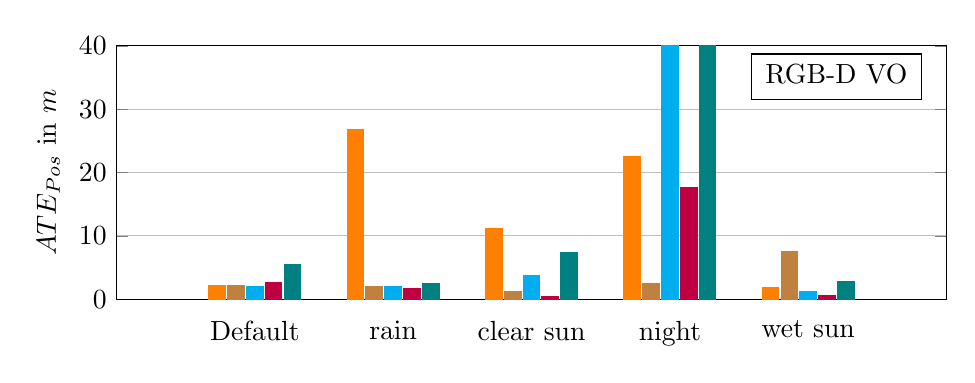
\begin{tikzpicture}
    \begin{axis}[
        width  = \textwidth,
        height = 4.8cm,
        ymax =40,
        major x tick style = transparent,
        ybar=2*\pgflinewidth,
        bar width=6pt,
        ymajorgrids = true,
        ylabel = {$ATE_{Pos}$ in $m$},
        % xlabel = {1 Default, 2 hard rain, 3 clear sunset, 4 clear night ,5 wet sunset},
        symbolic x coords={Default, rain, clear sun, night ,wet sun},
        xtick = data,
        scaled y ticks = false,
        enlarge x limits=0.25,
        ymin=0,
        legend pos=north east
    ]
    \addlegendimage{empty legend}
    \addlegendentry{RGB-D VO}

    \addplot[style={orange,fill=orange,mark=none}]
        coordinates {(Default, 2.10) (rain, 26.85) (clear sun, 11.109) (night , 22.593) (wet sun, 1.85)};
    
    \addplot[style={brown,fill=brown,mark=none}]
        coordinates {(Default, 2.16) (rain, 2.02) (clear sun, 1.28) (night , 2.518) (wet sun, 7.512)};
    
    \addplot[style={cyan,fill=cyan,mark=none}]
        coordinates {(Default, 1.94) (rain, 2.057) (clear sun, 3.768) (night , 75.997) (wet sun, 1.1535)};
    
    \addplot[style={purple,fill=purple,mark=none}]
        coordinates {(Default, 2.62) (rain, 1.648) (clear sun, 0.480) (night , 17.566) (wet sun, 0.52516)};
    
    \addplot[style={teal,fill=teal,mark=none}]
        coordinates {(Default, 5.55) (rain, 2.432) (clear sun, 7.2941) (night , 83.744) (wet sun, 2.789)};
    \end{axis}
  \end{tikzpicture}
	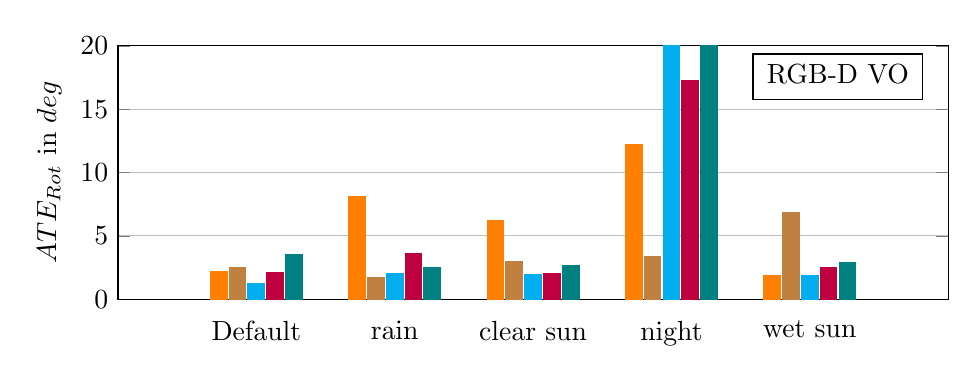
\begin{tikzpicture}
    \begin{axis}[
        width  = \textwidth,
        height = 4.8cm,
        ymax = 20,
        major x tick style = transparent,
        ybar=2*\pgflinewidth,
        bar width=6pt,
        ymajorgrids = true,
        ylabel = {$ATE_{Rot}$ in $deg$},
        % xlabel = {1 Default, 2 hard rain, 3 clear sunset, 4 clear night ,5 wet sunset},
        symbolic x coords={Default, rain, clear sun, night ,wet sun},
        xtick = data,
        scaled y ticks = false,
        enlarge x limits=0.25,
        ymin=0,
        legend pos=north east
    ]
    \addlegendimage{empty legend}
    \addlegendentry{RGB-D VO}
    \addplot[style={orange,fill=orange,mark=none}]
        coordinates {(Default, 2.21) (rain, 8.09) (clear sun, 6.195) (night ,12.18) (wet sun, 1.875)};
    
    \addplot[style={brown,fill=brown,mark=none}]
        coordinates {(Default,2.52) (rain, 1.73) (clear sun, 3.00) (night , 3.372) (wet sun, 6.825)};
    
    \addplot[style={cyan,fill=cyan,mark=none}]
        coordinates {(Default, 1.22) (rain, 2.00) (clear sun, 1.941) (night , 48.216) (wet sun, 1.838)};
    
    \addplot[style={purple,fill=purple,mark=none}]
        coordinates {(Default, 2.14) (rain, 3.60) (clear sun, 2.061) (night , 17.293) (wet sun, 2.518)};
    
    \addplot[style={teal,fill=teal,mark=none}]
        coordinates {(Default, 3.53) (rain, 2.493) (clear sun, 2.645) (night , 51.956) (wet sun, 2.893)};
    \end{axis}
  \end{tikzpicture}
	\caption[Absolute Trajectory Error (ATE) für RGB-D]{Absolute Trajectory Error (ATE) für RGB-D Visuelle Odometrie der geschätzten Translation und des geschätzten Winkels in Grad für alle 25 Testfahrten.}
\end{figure}

\begin{figure}[!ht]
	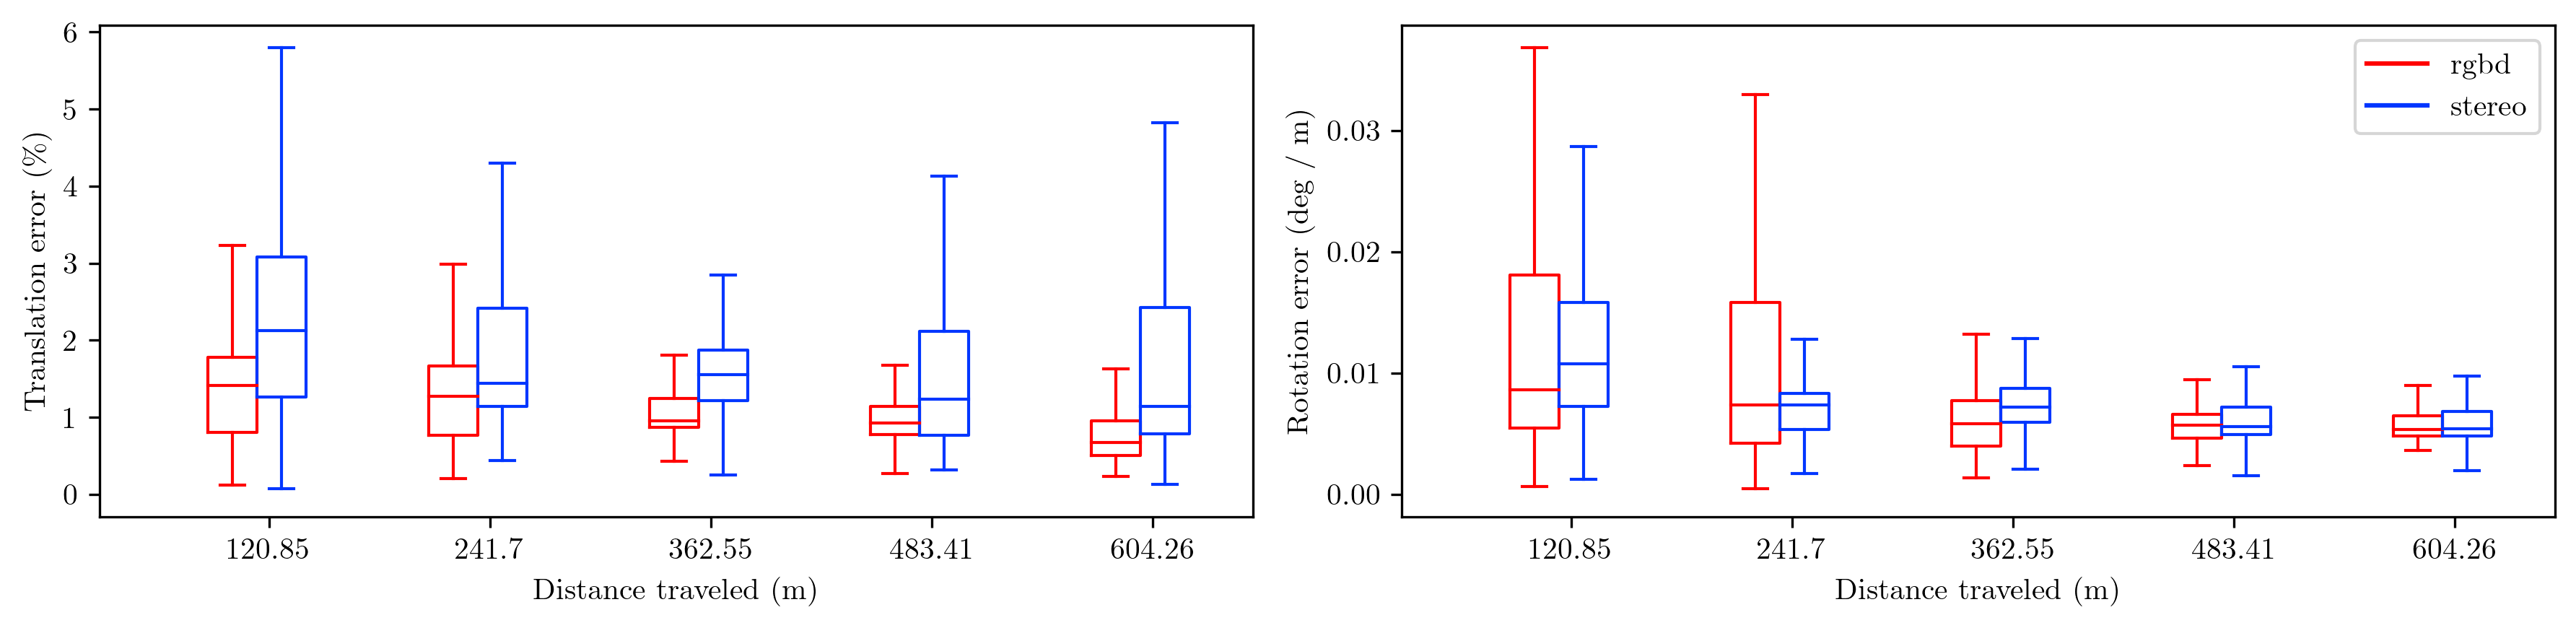
\includegraphics[width=\textwidth]{auswertung/trans_rot/default_04_trans_rot_error.png}\hfill
	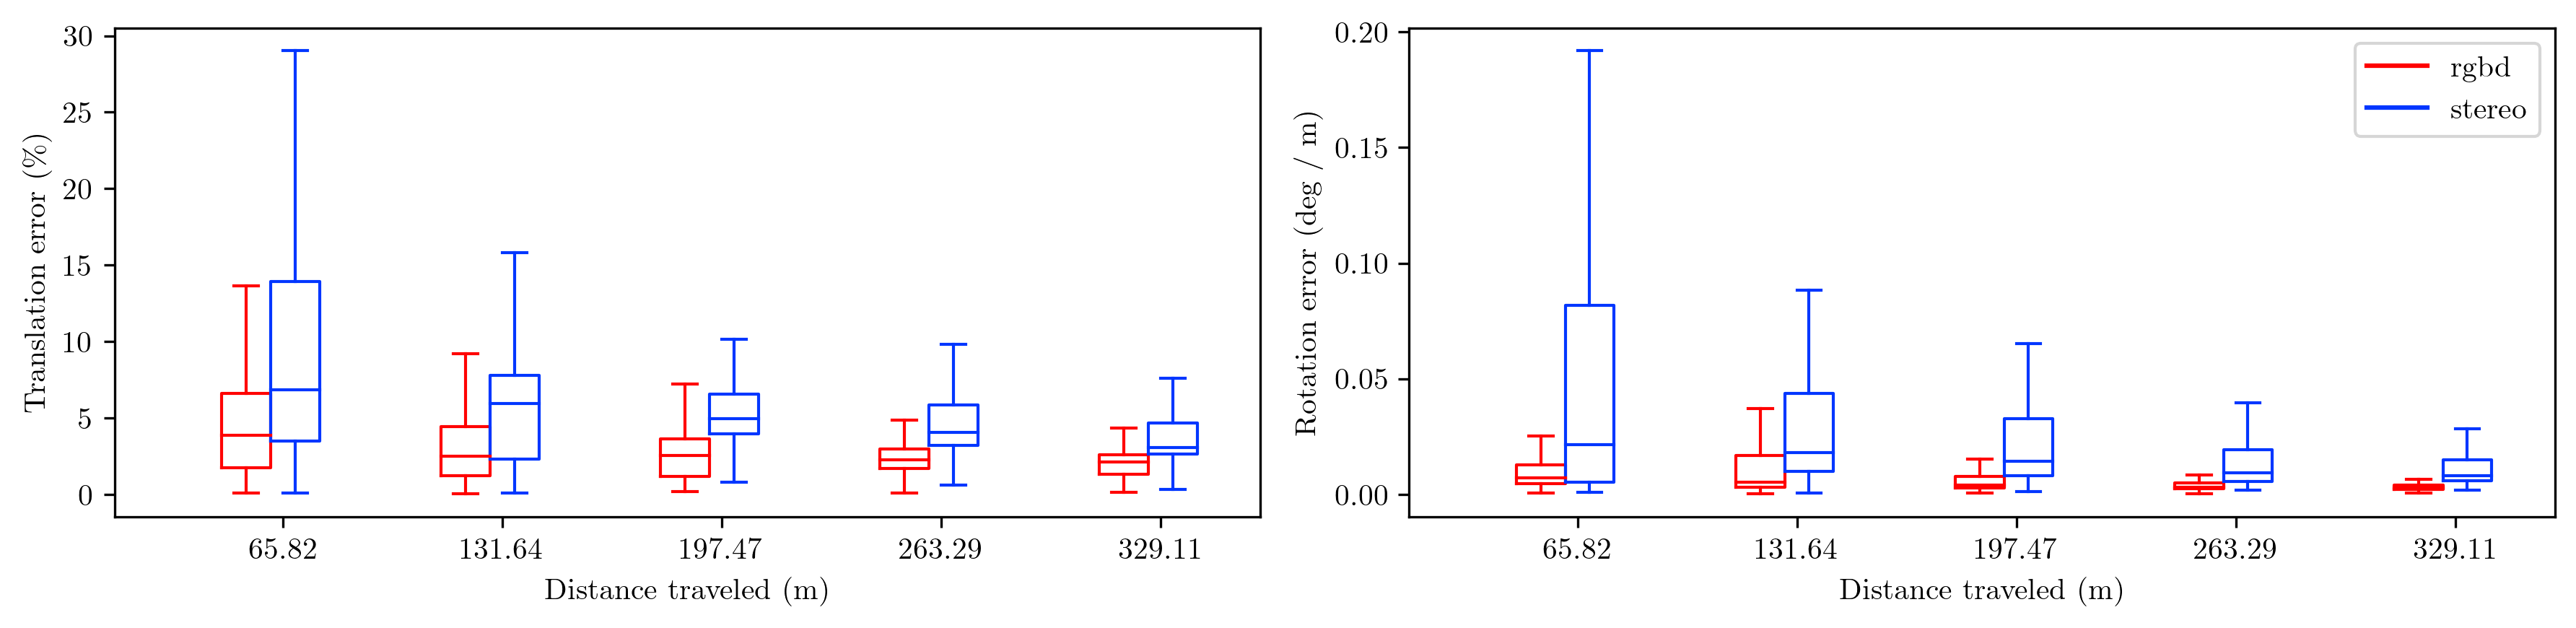
\includegraphics[width=\textwidth]{auswertung/trans_rot/hard_rain_03_trans_rot_error.png}\hfill
	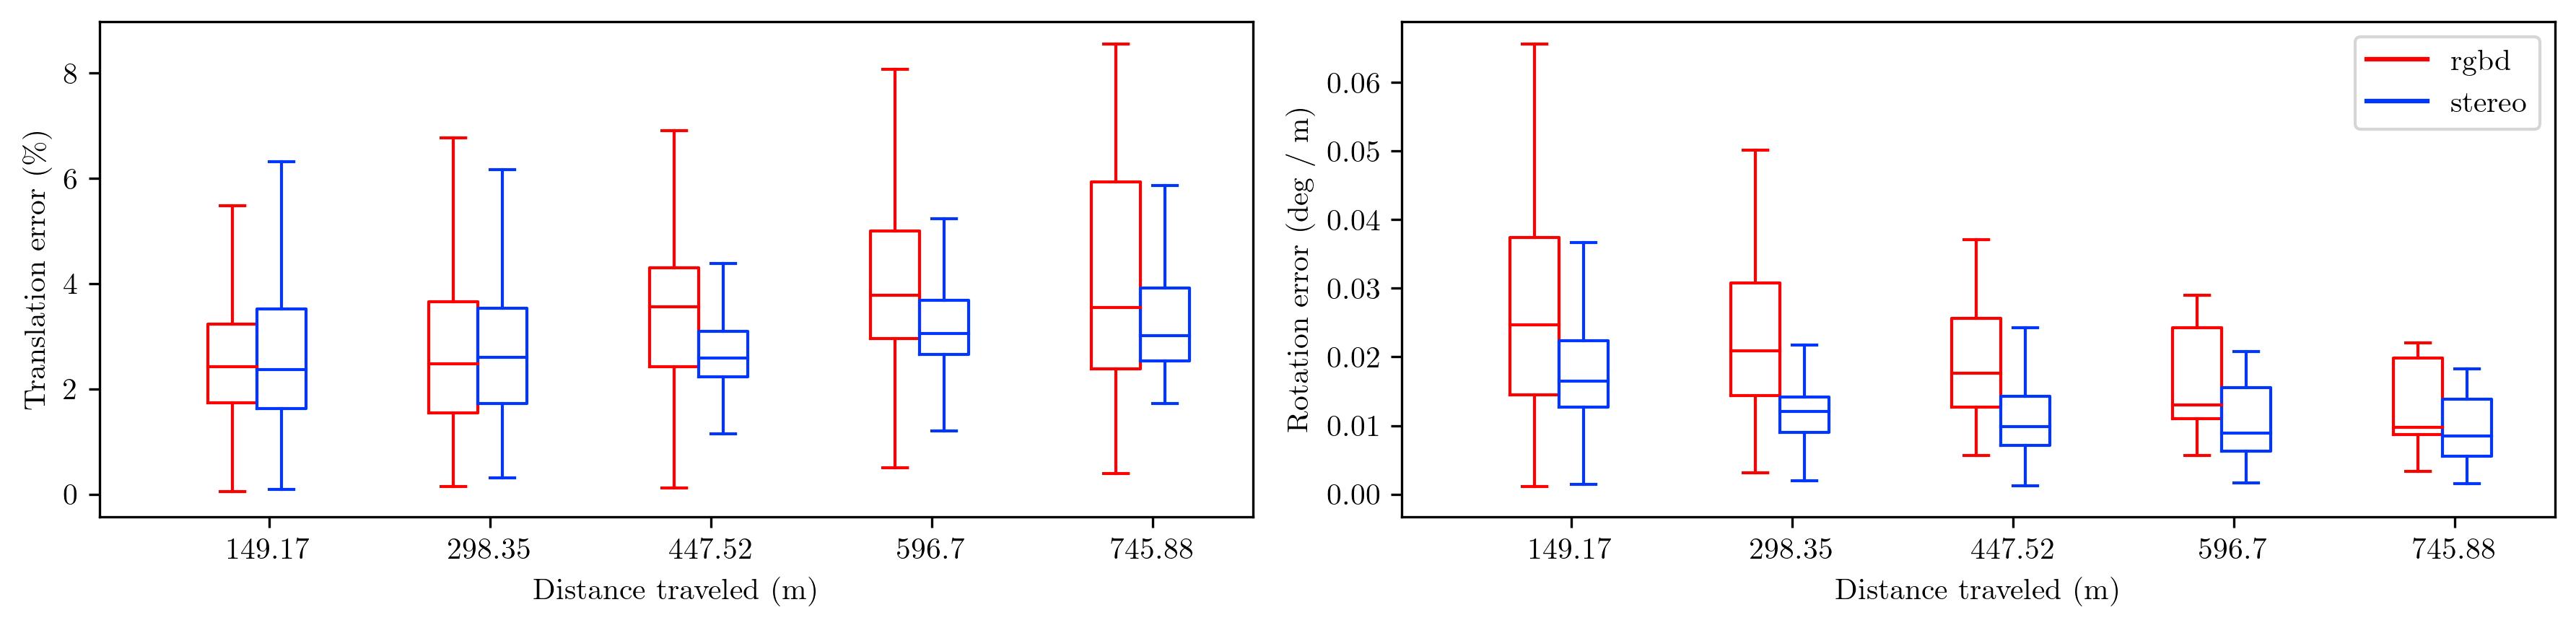
\includegraphics[width=\textwidth]{auswertung/trans_rot/sunset_01_trans_rot_error.png}
	\hfill
	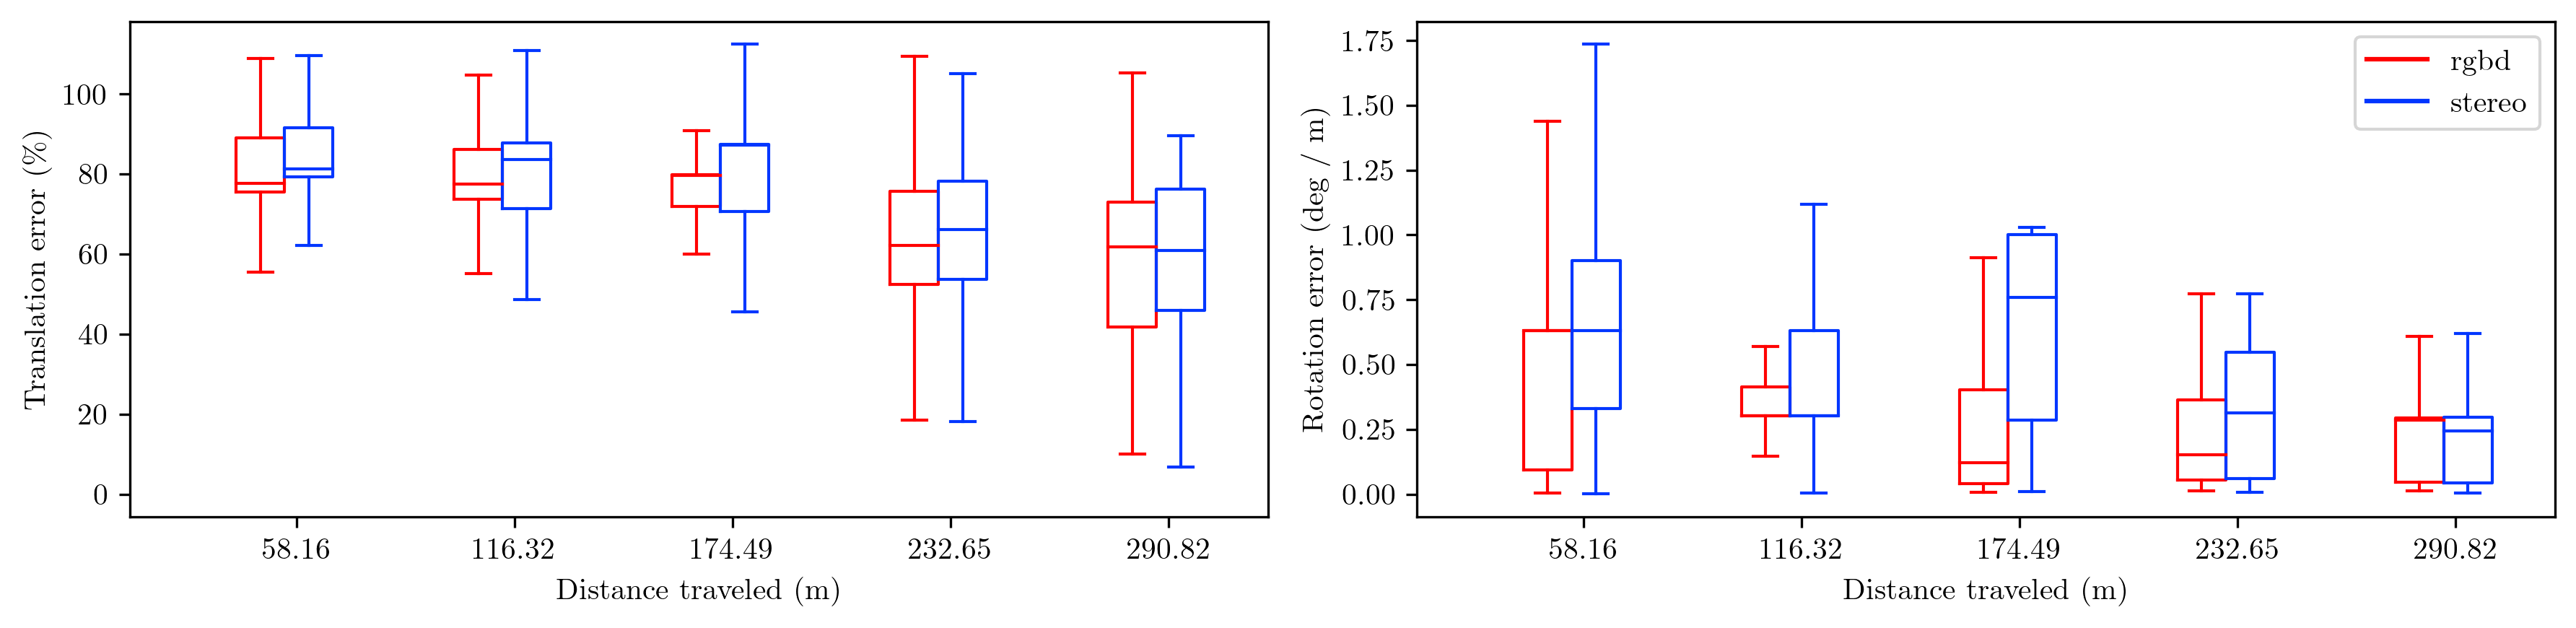
\includegraphics[width=\textwidth]{auswertung/trans_rot/clear_night_05_trans_rot_error.png}\hfill
	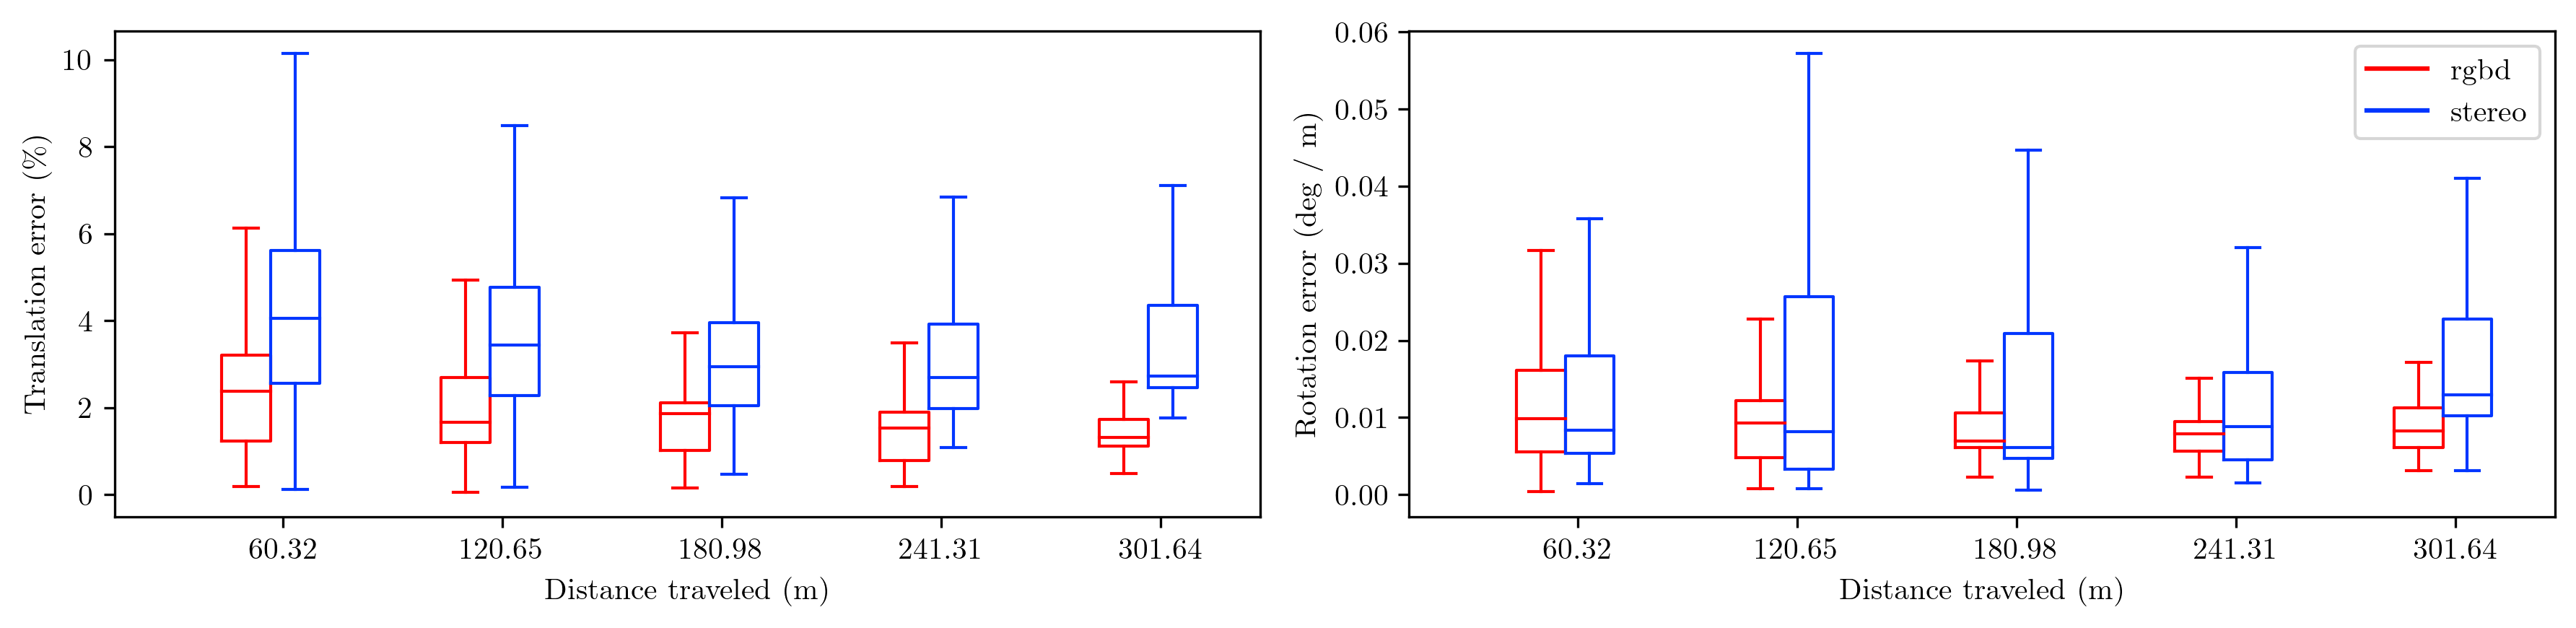
\includegraphics[width=\textwidth]{auswertung/trans_rot/wet_sunrise_01_trans_rot_error.png}\hfill
	\caption[Boxplots Absoluter Fehler von Streckenabschnitten]{Um den Trend in jedem Datensatz zu veranschaulichen wurden die Absoluten Fehler für je eine Strecke aus jedem Datensatz geplottet. Von oben nach unten: 1 Default, 2 hard rain, 3 clear sunset, 4 clear night, 5 wet sunset}
\end{figure}

\clearpage
\newpage

\begin{center}
		\begin{table}
  \centering
    \begin{tabular}{r|r|r|r|r|r}
      \toprule % <-- Toprule here
      \multicolumn{6}{c}{Median des relativen Rotations Fehlers in $deg/m$} \\
      \midrule % <-- Midrule here
      \phantom{abc} & Default & rain& clear sunset & night & wet sunset\\
      \midrule % <-- Midrule here
      (1) Stereo & 0.9452 & 4.0144 & 3.4640 & 2.9886& 2.1125\\
      \rowcolor{LightGray}
      (1) RGBD & 1.3338 & 3.1555 & 6.4847 &  0.8182& 1.5687\\
      (2) Stereo & 1.2672 & 1.0465 & 1.3600 & 3.2212& 2.1369\\
      \rowcolor{LightGray}
      (2) RGBD & 1.1546 & 1.0868 & 2.0310 &  2.5042& 1.0776\\
      (3) Stereo & 0.7136 & 1.8220 & 2.3278 & 36.9868& 0.7482\\
      \rowcolor{LightGray}
      (3) RGBD & 0.6619 &  1.6254 & 1.5180 & 38.5830& 1.1404\\
      (4) Stereo & 2.1637 &  2.4429 & 1.7825 & 53.7278& 2.4827\\
      \rowcolor{LightGray}
      (4) RGBD & 1.5119 &  3.3972 & 2.0200 & 11.9804& 2.5498\\
      (5) Stereo & 1.5989 & 4.1391 & 1.5751 & 167.3668& 1.2671\\
      \rowcolor{LightGray}
      (5) RGBD & 3.2175 & 2.1387 & 2.0686 & 34.6302&  1.8053\\	
      \bottomrule % <-- Bottomrule here
    \end{tabular}
  \caption{Median des relativer Fehlers der Rotation}
  \end{table} 	
  \begin{table}
    \centering
      \begin{tabular}{r|r|r|r|r|r}
        \toprule % <-- Toprule here
        \multicolumn{6}{c}{Median des Relativen Fehlers der Translation in $\%$} \\
        \midrule % <-- Midrule here
        \phantom{abc} & Default & rain& clear sunset & night & wet sunset\\
        \midrule % <-- Midrule here
        (1) Stereo &  2.2018 & 24.9510 & 6.8918 & 20.9637& 3.6919\\
        \rowcolor{LightGray}
        (1) RGBD & 1.6438 & 4.76527 & 9.4637 & 4.7189& 1.7361\\
        (2) Stereo & 2.4804 & 1.3636 & 0.9239 &  16.9190&  2.6304\\
        \rowcolor{LightGray}
        (2) RGBD & 1.8756 & 1.7771 & 0.9684 &  2.2069& 2.0401\\
        (3) Stereo & 1.4768 & 5.1681 & 4.1606 & 61.4019& 0.8780\\
        \rowcolor{LightGray}
        (3) RGBD & 1.2665 & 1.6829 & 3.2752 & 63.2587& 0.9144\\
        (4) Stereo & 2.6105 &  3.8872 & 0.0473 & 16.1462& 0.1121\\
        \rowcolor{LightGray}
        (4) RGBD & 2.1176 & 1.3754 &  0.1263 & 9.0187& 0.0566\\
        (5) Stereo &  17.3331 &  6.1409 & 3.4013 & 55.5880&0.9190\\
        \rowcolor{LightGray}
        (5) RGBD & 5.3631 &  1.4550 & 4.1606 & 48.8802& 2.2763\\	
        \bottomrule % <-- Bottomrule here
      \end{tabular}
    \caption{Median des Relativen Fehlers der Translation}
  \end{table} 		
\end{center}
\newpage
\begin{center}
		
  \begin{table}
    \centering
      \begin{tabular}{r|r|r|r|r|r}
        \toprule % <-- Toprule here
        \multicolumn{6}{c}{RMSE der Rotation in $deg/m$} \\
        \midrule % <-- Midrule here
        \phantom{abc} & Default & rain& clear sunset & night & wet sunset\\
        \midrule % <-- Midrule here
        (1) Stereo & 2.7334 & 14.5396 & 4.7107 & 29.6143& 8.2440\\
        \rowcolor{LightGray}
        (1) RGBD & 2.2146 & 8.0921 & 6.1959 & 12.1838& 1.8756\\
        (2) Stereo & 4.5297 & 7.6523 & 2.2452 & 20.4506& 8.5746\\
        \rowcolor{LightGray}
        (2) RGBD & 2.5232 & 1.7378 & 3.0055 & 3.3728& 6.8255\\
        (3) Stereo & 3.0501 & 6.7407 & 2.7294 & 52.7385& 2.1195\\
        \rowcolor{LightGray}
        (3) RGBD & 1.2257 & 2.0066 &  1.9411 & 48.2168& 1.8383\\
        (4) Stereo & 2.9097 & 6.4370 & 1.9908 & 58.5951& 3.0643\\
        \rowcolor{LightGray}
        (4) RGBD & 2.1487 & 3.6022 & 2.0612 & 17.2936&2.5188\\
        (5) Stereo & 19.5840 &  9.9986 & 4.2870 & 168.5980& 2.0029\\
        \rowcolor{LightGray}
        (5) RGBD & 3.2175 & 2.4937 & 2.6455 & 51.9567& 2.8930\\	
        \bottomrule % <-- Bottomrule here
      \end{tabular}
    \caption{RMSE der Rotation}
  \end{table} 	
  \begin{table}
    \centering
      \begin{tabular}{r|r|r|r|r|r}
        \toprule % <-- Toprule here
        \multicolumn{6}{c}{RMSE der Translation in $\%$} \\
        \midrule % <-- Midrule here
        \phantom{abc} & Default & rain& clear sunset & night & wet sunset\\
        \midrule % <-- Midrule here
        (1) Stereo & 2.7093 & 66.6148 & 10.7996 & 44.9045&  22.2712\\
        \rowcolor{LightGray}
        (1) RGBD & 2.1084 & 26.8571 &11.1097 & 22.5937& 1.8512\\
        (2) Stereo & 2.6822 & 16.9418 & 1.1682 & 24.9654& 9.4863\\
        \rowcolor{LightGray}
        (2) RGBD &  2.1633 & 2.0260 & 1.2843 & 2.5186& 7.5126\\
        (3) Stereo & 8.0751 & 26.6375 & 4.6390 & 86.9499& 1.2902\\
        \rowcolor{LightGray}
        (3) RGBD & 1.9449 & 2.0570 & 3.76853 & 75.9970& 1.1535\\
  
        (4) Stereo & 12.2844 & 14.1325 &  0.5691 & 21.3222& 0.6728\\
        \rowcolor{LightGray}
        (4) RGBD & 2.6251 & 1.6480 & 0.4805 & 17.5666& 0.5251\\
        (5) Stereo & 28.2357 & 18.8744 & 9.7872 & 91.4595& 1.2994\\
        \rowcolor{LightGray}
        (5) RGBD & 5.5522 & 2.4321 & 7.2941 & 83.7440&  2.7893\\	
        \bottomrule % <-- Bottomrule here
      \end{tabular}
    \caption{RMSE der Translation}
  \end{table} 		
\end{center}

\newpage
\clearpage
\newpage

\section{Diskussion}
Die RMSE Tabellen zeigen die Standardabweichung für die Schätzfehler der beiden Visuellen Odometrie Systeme RGB-D und Stereo Kamera. Die Standardabweichung zeigt wie sehr die Schätzungen um den Mittelwert Streuen. Die Median Tabellen zeigen die gemittelten Fehlerwerte mit geringeren Bewertung für Ausrei{\ss}er.
\newline 

Es ist sofort ersichtlich, dass die implementierte visuelle Odometrie unbrauchbare Ergebnisse für Nachtfahrten liefert. Es wäre interessant zu sehen, in wie fern sich die Ergebnisse für Fahrten mit Frontscheinwerfern ändern. Da Stra{\ss}en, insbesondere Asphalt, eine Textur arme Oberflächentextur bieten, würden die Kamerabilder aus der RGB Kamera vermutlich dennoch nicht genug Merkmale beinhalten.   
\newline 

Der Schätzfehler mit Stereokamera streut stärker als für den RGB-D au{\ss}er für 'Clear Sunset' wo ein sehr niedriger Sonnenstand vorherrscht.  
\newline

In der Auswertung des Gesamtstreckenfehlers zeigt sich, dass der RGB-D Kameraaufbau insgesamt kleinere Schätzfehler hat. Mit weniger Streuung ist es auch das Robustere System.    
\newline

Keines der Systeme zeigte Auffälligkeiten bei Ein- und Ausfahrten des in der Karte integrierten Tunnel. Bei hohen Geschwindigkeiten $(> 80 km\/h)$ kam es vermehrt zum Verlust der Schätzung, vor allem auf Streckenabschnitten mit wenigen markanten Umgebungsmerkmalen.  
\newline

Insgesamt konnte gezeigt werden, dass eine Lokalisierung des Fahrzeugs alleine durch Visuelle Odmometrie erfolgreich durchgeführt werden konnte. Beide Systeme liefern i.d.R. bei Tageslicht weniger als 10 Grad Winkelfehler. Die Visuelle Odometrie mit RGB-D Kamera schafft in 17 von 25 Teststrecken einen einen Absoluten Streckenfehler von weniger als 5 Metern. 

\section{Ausblick}
Das System kann als Front-End für einen SLAM Algorithmus verwendet werden. Bei einigen Testfahrten hat sich die Odometrie von einer gro{\ss}en Fehlschätzung vor allem nie 'erholt', vor allem dann, wenn der Fehler zu Beginn auftrat. Durch SLAM könnten solche Verläufe stabilisiert werden und das gesamte Verfahren würde Robuster werden. 
\newline

Eine weitere, naheliegende Möglichkeit wäre eine Sensorfusion mit einer IMU. Sogenannte Visual Inertial Odometry zeigt in aktuellen Forschungsergebnissen mehrere Paper gute Ergebnisse für eine Fehlerkorrektur und damit eine Reduktion der Drift.

% \begin{appendix}
%   %%
%% Beuth Hochschule für Technik --  Abschlussarbeit
%%
%% Anhang
%%
%%%%%%%%%%%%%%%%%%%%%%%%%%%%%%%%%%%%%%%%%%%%%%%%%%%%%%%%%%%%%%%%%%%%%


\chapter{Angehängtes: Die Dateien des Pakets}


\subsection*{Stylefile}
Die  Styledatei für diese  Abschlussarbeit ist  \texttt{bhtThesis.sty}, die  in der
Archivdatei vorliegt.  Diese muss von \LaTeX\  auffindbar sein, muss  also in einem
\LaTeX\ bekannten Ordner liegen:
\begin{itemize}
\item Ubuntu-Linux: \verb|$HOME/texmf/tex/latex/bhtThesis/bhtThesis.sty|
\item MikTeX: \verb|c:\localtexmf\tex\latex\bhtThesis/bhtThesis.sty|
\end{itemize}


\subsection*{Beispieldokument}
Dieses  Dokument befindet sich  im Unterordner  \texttt{tryout} des  zip-files. Sie
können diese  Dateien in  einen Ordner kopieren,  in dem Sie  schliesslich arbeiten
werden. Die Dateien sind die folgenden

\begin{itemize}
\item \texttt{abstract\_de.tex} Kurzfassung in deutscher Sprache
\item \texttt{abstract\_en.tex} Kurzfassung in englischer Sprache
\item \texttt{anhang.tex} der Anhang
\item \texttt{bhtThesis.bib} beinhaltet die zu zitierenden Literaturstellen und
  wird von bib\TeX ausgewertet 
\item \texttt{main.pdf} ist die Ausgabendatei mit der Druckvorlage
\item \texttt{main.tex} beinhaltet das Hauptdokument
\item \texttt{makefile} realsiert das automatische mehrfache Übersetzen, hierfür
  muss \texttt{make} auf dem System installiert sein.
\item \texttt{myapalike.bst} beinhaltet die Formatierung für das
  Literaturverzeichnis 
\item \texttt{personalMacros.tex} kann einzelne, persönliche Macros beinhalten, die
  das Schreiben erleichtern
\item \texttt{titelseiten.tex} realisiert alle Seiten bis zum Beginn des ersten
  Abschnittes  

\item Ordner \texttt{pictures}
  \begin{itemize}
  \item \texttt{BHT-Logo-Basis.eps}
  \item \texttt{BHT-Logo-Basis.pdf}
  \end{itemize}

\item Ordner \texttt{kapitel1}
  \begin{itemize}
  \item \texttt{ch1.tex} Quelltext des Kapitel 1
  \item Ordner \texttt{pictures}
    \begin{itemize}
    \item \texttt{schaltbild.pdf}
    \end{itemize}
  \end{itemize}
  
\item Ordner \texttt{kapitel2}
  \begin{itemize}
  \item \texttt{ch2.tex} Quelltext des Kapitel 2
  \item Ordner \texttt{pictures}
    \begin{itemize}
    \item leer
    \end{itemize}
  \end{itemize}  
\end{itemize}


% \end{appendix}
%%%%%%%%%%%%%%%%%%%%%%%%%%%%%%%%%%%%%%%%%%%%%%%%%%%%%%%%%%%%%%%
%% Literaturverzeichnis

\clearpage\newpage
\addcontentsline{toc}{chapter}{Literatur- und Quellenverzeichnis}
\bibliographystyle{unsrt}
%\bibliographystyle{myapalike}
\bibliography{bhtThesis}

\end{document}